\chapter{CXCORE}

\section{Basic Structures}

\subsection{Basic Structures}

\cvstruct{CvPoint}\label{CvPoint}

2D point with integer coordinates (usually zero-based)

\begin{lstlisting}
typedef struct CvPoint
{
    int x; 
    int y; 
}
CvPoint;
\end{lstlisting}

\begin{description}
\cvarg{x}{x-coordinate}
\cvarg{y}{y-coordinate} 
\end{description}

\begin{lstlisting}
/* Constructor */
inline CvPoint cvPoint( int x, int y );

/* Conversion from CvPoint2D32f */
inline CvPoint cvPointFrom32f( CvPoint2D32f point );
\end{lstlisting}

\cvstruct{CvPoint2D32f}\label{CvPoint2D32f}

2D point with floating-point coordinates

\begin{lstlisting}

typedef struct CvPoint2D32f
{
    float x;
    float y; 
}
CvPoint2D32f;
\end{lstlisting}

\begin{description}
\cvarg{x}{x-coordinate}
\cvarg{y}{y-coordinate}
\end{description}

\begin{lstlisting}
/* Constructor */
inline CvPoint2D32f cvPoint2D32f( double x, double y );

/* Conversion from CvPoint */
inline CvPoint2D32f cvPointTo32f( CvPoint point );

\end{lstlisting}


\cvstruct{CvPoint3D32f}\label{CvPoint3D32f}

3D point with floating-point coordinates

\begin{lstlisting}

typedef struct CvPoint3D32f
{
    float x; 
    float y; 
    float z; 
}
CvPoint3D32f;
\end{lstlisting}

\begin{description}
\cvarg{x}{x-coordinate}
\cvarg{y}{y-coordinate}
\cvarg{z}{z-coordinate}
\end{description}

\begin{lstlisting}
/* Constructor */
inline CvPoint3D32f cvPoint3D32f( double x, double y, double z );

\end{lstlisting}

\cvstruct{CvPoint2D64f}\label{CvPoint2D64f}

2D point with double precision floating-point coordinates

\begin{lstlisting}

typedef struct CvPoint2D64f
{
    double x; 
    double y; 
}
CvPoint2D64f;
\end{lstlisting}

\begin{description}
\cvarg{x}{x-coordinate}
\cvarg{y}{y-coordinate}
\end{description}

\begin{lstlisting}
/* Constructor */
inline CvPoint2D64f cvPoint2D64f( double x, double y );

/* Conversion from CvPoint */
inline CvPoint2D64f cvPointTo64f( CvPoint point );

\end{lstlisting}

\cvstruct{CvPoint3D64f}\label{CvPoint3D64f}

3D point with double precision floating-point coordinates

\begin{lstlisting}

typedef struct CvPoint3D64f
{
    double x; 
    double y; 
    double z; 
}
CvPoint3D64f;
\end{lstlisting}

\begin{description}
\cvarg{x}{x-coordinate}
\cvarg{y}{y-coordinate}
\cvarg{z}{z-coordinate}
\end{description}

\begin{lstlisting}
/* Constructor */
inline CvPoint3D64f cvPoint3D64f( double x, double y, double z );

\end{lstlisting}

\cvstruct{CvSize}\label{CvSize}

Pixel-accurate size of a rectangle.

\begin{lstlisting}

typedef struct CvSize
{
    int width; 
    int height; 
}
CvSize;
\end{lstlisting}

\begin{description}
\cvarg{width}{Width of the rectangle}
\cvarg{height}{Height of the rectangle}
\end{description}

\begin{lstlisting}
/* Constructor */
inline CvSize cvSize( int width, int height );

\end{lstlisting}

\cvstruct{CvSize2D32f}\label{CvSize2D32f}

Sub-pixel accurate size of a rectangle.

\begin{lstlisting}

typedef struct CvSize2D32f
{
    float width; 
    float height; 
}
CvSize2D32f;
\end{lstlisting}

\begin{description}
\cvarg{width}{Width of the rectangle}
\cvarg{height}{Height of the rectangle}
\end{description}

\begin{lstlisting}
/* Constructor */
inline CvSize2D32f cvSize2D32f( double width, double height );

\end{lstlisting}

\cvstruct{CvRect}\label{CvRect}

Offset (usually the top-left corner) and size of a rectangle.

\begin{lstlisting}

typedef struct CvRect
{
    int x; 
    int y; 
    int width; 
    int height; 
}
CvRect;
\end{lstlisting}

\begin{description}
\cvarg{x}{x-coordinate of the top-left corner}
\cvarg{y}{y-coordinate of the top-left corner (bottom-left for Windows bitmaps)}
\cvarg{width}{Width of the rectangle}
\cvarg{height}{Height of the rectangle}
\end{description}

\begin{lstlisting}
/* Constructor */
inline CvRect cvRect( int x, int y, int width, int height );

\end{lstlisting}

\cvstruct{CvScalar}\label{CvScalar}

A container for 1-,2-,3- or 4-tuples of doubles.

\begin{lstlisting}

typedef struct CvScalar
{
    double val[4];
}
CvScalar;

\end{lstlisting}

\begin{lstlisting}
/* Constructor: 
initializes val[0] with val0, val[1] with val1, etc. 
*/
inline CvScalar cvScalar( double val0, double val1=0,
                          double val2=0, double val3=0 );
/* Constructor: 
initializes all of val[0]...val[3] with val0123 
*/
inline CvScalar cvScalarAll( double val0123 );

/* Constructor: 
initializes val[0] with val0, and all of val[1]...val[3] with zeros 
*/
inline CvScalar cvRealScalar( double val0 );

\end{lstlisting}

\cvstruct{CvTermCriteria}\label{CvTermCriteria}

Termination criteria for iterative algorithms.

\begin{lstlisting}

#define CV_TERMCRIT_ITER    1
#define CV_TERMCRIT_NUMBER  CV_TERMCRIT_ITER
#define CV_TERMCRIT_EPS     2

typedef struct CvTermCriteria
{
    int    type;
    int    max_iter; 
    double epsilon; 
}
CvTermCriteria;
\end{lstlisting}

\begin{description}
\cvarg{type}{A combination of CV\_TERMCRIT\_ITER and CV\_TERMCRIT\_EPS}
\cvarg{max\_iter}{Maximum number of iterations}
\cvarg{epsilon}{Required accuracy}
\end{description}

\begin{lstlisting}
/* Constructor */
inline CvTermCriteria cvTermCriteria( int type, int max_iter, double epsilon );

/* Check and transform a CvTermCriteria so that 
   type=CV_TERMCRIT_ITER+CV_TERMCRIT_EPS
   and both max_iter and epsilon are valid */
CvTermCriteria cvCheckTermCriteria( CvTermCriteria criteria,
                                    double default_eps,
                                    int default_max_iters );

\end{lstlisting}

\cvstruct{CvMat}\label{CvMat}

A multi-channel matrix.

\begin{lstlisting}

typedef struct CvMat
{
    int type; 
    int step; 

    int* refcount; 

    union
    {
        uchar* ptr;
        short* s;
        int* i;
        float* fl;
        double* db;
    } data; 

#ifdef __cplusplus
    union
    {
        int rows;
        int height;
    };

    union
    {
        int cols;
        int width;
    };
#else
    int rows; 
    int cols; 
#endif

} CvMat;

\end{lstlisting}

\begin{description}
\cvarg{type}{A CvMat signature (CV\_MAT\_MAGIC\_VAL) containing the type of elements and flags}
\cvarg{step}{Full row length in bytes}
\cvarg{refcount}{Underlying data reference counter}
\cvarg{data}{Pointers to the actual matrix data}
\cvarg{rows}{Number of rows}
\cvarg{cols}{Number of columns}
\end{description}


Matrices are stored row by row. All of the rows are aligned by 4 bytes.


\cvstruct{CvMatND}\label{CvMatND}

Multi-dimensional dense multi-channel array.

\begin{lstlisting}

typedef struct CvMatND
{
    int type; 
    int dims;

    int* refcount; 

    union
    {
        uchar* ptr;
        short* s;
        int* i;
        float* fl;
        double* db;
    } data; 

    struct
    {
        int size;
        int step;
    }
    dim[CV_MAX_DIM];

} CvMatND;

\end{lstlisting}

\begin{description}
\cvarg{type}{A CvMatND signature (CV\_MATND\_MAGIC\_VAL), combining the type of elements and flags}
\cvarg{dims}{The number of array dimensions}
\cvarg{refcount}{Underlying data reference counter}
\cvarg{data}{Pointers to the actual matrix data}
\cvarg{dim}{For each dimension, the pair (number of elements, distance between elements in bytes)}
\end{description}

\cvstruct{CvSparseMat}\label{CvSparseMat}

Multi-dimensional sparse multi-channel array.

\begin{lstlisting}

typedef struct CvSparseMat
{
    int type;
    int dims; 
    int* refcount; 
    struct CvSet* heap; 
    void** hashtable; 
    int hashsize;
    int total; 
    int valoffset; 
    int idxoffset; 
    int size[CV_MAX_DIM]; 

} CvSparseMat;

\end{lstlisting}

\begin{description}
\cvarg{type}{A CvSparseMat signature (CV\_SPARSE\_MAT\_MAGIC\_VAL), combining the type of elements and flags.}
\cvarg{dims}{Number of dimensions}
\cvarg{refcount}{Underlying reference counter. Not used.}
\cvarg{heap}{A pool of hash table nodes}
\cvarg{hashtable}{The hash table. Each entry is a list of nodes.}
\cvarg{hashsize}{Size of the hash table}
\cvarg{total}{Total number of sparse array nodes}
\cvarg{valoffset}{The value offset of the array nodes, in bytes}
\cvarg{idxoffset}{The index offset of the array nodes, in bytes}
\cvarg{size}{Array of dimension sizes}
\end{description}

\cvstruct{IplImage}\label{IplImage}

IPL image header

\begin{lstlisting}

typedef struct _IplImage
{
    int  nSize;         
    int  ID;            
    int  nChannels;     
    int  alphaChannel;  
    int  depth;         
    char colorModel[4]; 
    char channelSeq[4]; 
    int  dataOrder;     
    int  origin;        
    int  align;         
    int  width;         
    int  height;        
    struct _IplROI *roi; 
    struct _IplImage *maskROI; 
    void  *imageId;     
    struct _IplTileInfo *tileInfo; 
    int  imageSize;                             
    char *imageData;  
    int  widthStep;   
    int  BorderMode[4]; 
    int  BorderConst[4]; 
    char *imageDataOrigin; 
}
IplImage;

\end{lstlisting}

\begin{description}
\cvarg{nSize}{\texttt{sizeof(IplImage)}}
\cvarg{ID}{Version, always equals 0}
\cvarg{nChannels}{Number of channels. Most OpenCV functions support 1-4 channels.}
\cvarg{alphaChannel}{Ignored by OpenCV}
\cvarg{depth}{Pixel depth in bits. The supported depths are:
\begin{description}
\cvarg{IPL\_DEPTH\_8U}{Unsigned 8-bit integer}
\cvarg{IPL\_DEPTH\_8S}{Signed 8-bit integer}
\cvarg{IPL\_DEPTH\_16U}{Unsigned 16-bit integer}
\cvarg{IPL\_DEPTH\_16S}{Signed 16-bit integer}
\cvarg{IPL\_DEPTH\_32S}{Signed 32-bit integer}
\cvarg{IPL\_DEPTH\_32F}{Single-precision floating point}
\cvarg{IPL\_DEPTH\_64F}{Double-precision floating point}
\end{description}}
\cvarg{colorModel}{Ignored by OpenCV. The OpenCV function \cross{CvtColor} requires the source and destination color spaces as parameters.}
\cvarg{channelSeq}{Ignored by OpenCV}
\cvarg{dataOrder}{0 = \texttt{IPL\_DATA\_ORDER\_PIXEL} - interleaved color channels, 1 - separate color channels. \cross{CreateImage} only creates images with interleaved channels. For example, the usual layout of a color image is: $ b_{00} g_{00} r_{00} b_{10} g_{10} r_{10} ...$}
\cvarg{origin}{0 - top-left origin, 1 - bottom-left origin (Windows bitmap style)}
\cvarg{align}{Alignment of image rows (4 or 8). OpenCV ignores this and uses widthStep instead.}
\cvarg{width}{Image width in pixels}
\cvarg{height}{Image height in pixels}
\cvarg{roi}{Region Of Interest (ROI). If not NULL, only this image region will be processed.}
\cvarg{maskROI}{Must be NULL in OpenCV}
\cvarg{imageId}{Must be NULL in OpenCV}
\cvarg{tileInfo}{Must be NULL in OpenCV}
\cvarg{imageSize}{Image data size in bytes. For interleaved data, this equals $\texttt{image->height} \cdot \texttt{image->widthStep}$ }
\cvarg{imageData}{A pointer to the aligned image data}
\cvarg{widthStep}{The size of an aligned image row, in bytes}
\cvarg{BorderMode}{Border completion mode, ignored by OpenCV}
\cvarg{BorderConst}{Border completion mode, ignored by OpenCV}
\cvarg{imageDataOrigin}{A pointer to the origin of the image data (not necessarily aligned). This is used for image deallocation.}
\end{description}

The \cross{IplImage} structure was inherited from the Intel Image Processing Library, in which the format is native. OpenCV only supports a subset of possible \cross{IplImage} formats, as outlined in the parameter list above.

In addition to the above restrictions, OpenCV handles ROIs differently. OpenCV functions require that the image size or ROI size of all source and destination images match exactly. On the other hand, the Intel Image Processing Library processes the area of intersection between the source and destination images (or ROIs), allowing them to vary independently. 

\cvstruct{CvArr}\label{CvArr}

Arbitrary array

\begin{lstlisting}

typedef void CvArr;

\end{lstlisting}

The metatype \texttt{CvArr} is used \textit{only} as a function parameter to specify that the function accepts arrays of multiple types, such as IplImage*, CvMat* or even CvSeq*. The particular array type is determined at runtime by analyzing the first 4 bytes of the header.


\section{Operations on Arrays}

\subsection{Initialization}

\cvfunc{CreateImage}\label{CreateImage}

Creates an image header and allocates the image data.

\cvexp{
IplImage* cvCreateImage( 

CvSize size, 

int depth, 

int channels );
}{CPP}{CreateImage(size, depth, channels)->image}

\begin{description}
\cvarg{size}{Image width and height}
\cvarg{depth}{Bit depth of image elements. See \cross{IplImage} for valid depths.}
\cvarg{channels}{Number of channels per pixel. See \cross{IplImage} for details. This function only creates images with interleaved channels.}
\end{description}

This call is a shortened form of

\begin{lstlisting}
header = cvCreateImageHeader( size, depth, channels );
cvCreateData( header );
\end{lstlisting}


\cvfunc{CreateImageHeader}\label{CreateImageHeader}

Creates an image header but does not allocate the image data.

\cvexp{
IplImage* cvCreateImageHeader( 

CvSize size, 

int depth, 

int channels );
}{CPP}{PYTHON}

\begin{description}
\cvarg{size}{Image width and height}
\cvarg{depth}{Image depth (see \cross{CreateImage})}
\cvarg{channels}{Number of channels (see \cross{CreateImage})}
\end{description}

This call is an analogue of

\begin{lstlisting}
iplCreateImageHeader( channels, 0, depth,
                      channels == 1 ? "GRAY" : "RGB",
                      channels == 1 ? "GRAY" : channels == 3 ? "BGR" :
                      channels == 4 ? "BGRA" : "",
                      IPL_DATA_ORDER_PIXEL, IPL_ORIGIN_TL, 4,
                      size.width, size.height,
                      0,0,0,0);
\end{lstlisting}

but it does not use IPL functions by default (see the \texttt{CV\_TURN\_ON\_IPL\_COMPATIBILITY} macro).

\cvfunc{ReleaseImageHeader}\label{ReleaseImageHeader}

Deallocates an image header.

\cvexp{
void cvReleaseImageHeader( IplImage** image );
}{CPP}{PYTHON}

\begin{description}
\cvarg{image}{Double pointer to the image header}
\end{description}

This call is an analogue of

\begin{lstlisting}
if( image )
{
    iplDeallocate( *image, IPL_IMAGE_HEADER | IPL_IMAGE_ROI );
    *image = 0;
}
\end{lstlisting}

but it does not use IPL functions by default (see the \texttt{CV\_TURN\_ON\_IPL\_COMPATIBILITY} macro).


\cvfunc{ReleaseImage}\label{ReleaseImage}

Deallocates the image header and the image data.

\cvexp{

void cvReleaseImage( IplImage** image );

}{CPP}{PYTHON}

\begin{description}
\cvarg{image}{Double pointer to the image header}
\end{description}

This call is a shortened form of

\begin{lstlisting}

if( *image )
{
    cvReleaseData( *image );
    cvReleaseImageHeader( image );
}

\end{lstlisting}


\cvfunc{InitImageHeader}\label{InitImageHeader}

Initializes an image header that was previously allocated.

\cvexp{

IplImage* cvInitImageHeader( \par IplImage* image,\par CvSize size,\par int depth,\par int channels,\par int origin=0,\par int align=4 );

}{CPP}{PYTHON}

\begin{description}
\cvarg{image}{Image header to initialize}
\cvarg{size}{Image width and height}
\cvarg{depth}{Image depth (see \cross{CreateImage})}
\cvarg{channels}{Number of channels (see \cross{CreateImage})}
\cvarg{origin}{Top-left \texttt{IPL\_ORIGIN\_TL} or bottom-left \texttt{IPL\_ORIGIN\_BL}}
\cvarg{align}{Alignment for image rows, typically 4 or 8 bytes}
\end{description}

The returned \texttt{IplImage*} points to the initialized header.

\cvfunc{CloneImage}\label{CloneImage}

Makes a full copy of an image, including the header, data, and ROI.

\cvexp{

IplImage* cvCloneImage( const IplImage* image );

}{CPP}{CloneImage(image)-> copy}

\begin{description}
\cvarg{image}{The original image}
\end{description}

The returned \texttt{IplImage*} points to the image copy.

\cvfunc{SetImageCOI}\label{SetImageCOI}

Sets the channel of interest in an IplImage.

\cvexp{

void cvSetImageCOI( \par IplImage* image,\par int coi );

}{CPP}{SetImageCOI(image, coi)-> None}

\begin{description}
\cvarg{image}{A pointer to the image header}
\cvarg{coi}{The channel of interest. 0 - all channels are selected, 1 - first channel is selected, etc. Note that the channel indices become 1-based.}
\end{description}

If the ROI is set to \texttt{NULL} and the coi is \textit{not} 0,
the ROI is allocated. Most OpenCV functions do \textit{not} support
the COI setting, so to process an individual image/matrix channel one
may copy (via \cross{Copy} or \cross{Split}) the channel to a separate
image/matrix, process it and then copy the result back (via \cross{Copy}
or \cross{Merge}) if needed.

\cvfunc{GetImageCOI}\label{GetImageCOI}

Returns the index of the channel of interest. 

\cvexp{

int cvGetImageCOI( const IplImage* image );

}{CPP}{GetImageCOI(image)-> channel}

\begin{description}
\cvarg{image}{A pointer to the image header}
\end{description}

Returns the channel of interest of in an IplImage. Returned values correspond to the \texttt{coi} in \cross{SetImageCOI}.

\cvfunc{SetImageROI}\label{SetImageROI}

Sets an image Region Of Interest (ROI) for a given rectangle.

\cvexp{

void cvSetImageROI( \par IplImage* image,\par CvRect rect );

}{CPP}{SetImageROI(image, rect)-> None}

\begin{description}
\cvarg{image}{A pointer to the image header}
\cvarg{rect}{The ROI rectangle}
\end{description}

If the original image ROI was \texttt{NULL} and the \texttt{rect} is not the whole image, the ROI structure is allocated.

Most OpenCV functions support the use of ROI and treat the image rectangle as a separate image. For example, all of the pixel coordinates are counted from the top-left (or bottom-left) corner of the ROI, not the original image.

\cvfunc{ResetImageROI}\label{ResetImageROI}

Resets the image ROI to include the entire image and releases the ROI structure.

\cvexp{

void cvResetImageROI( IplImage* image );

}{CPP}{ResetImageROI(image)-> None}

\begin{description}
\cvarg{image}{A pointer to the image header}
\end{description}

This produces a similar result to the following, but in addition it releases the ROI structure.

\begin{lstlisting}

cvSetImageROI( image, cvRect( 0, 0, image->width, image->height ));
cvSetImageCOI( image, 0 );

\end{lstlisting}


\cvfunc{GetImageROI}\label{GetImageROI}

Returns the image ROI.

\cvexp{

CvRect cvGetImageROI( const IplImage* image );

}{CPP}{GetImageROI(image)-> CvRect}

\begin{description}
\cvarg{image}{A pointer to the image header}
\end{description}


If there is no ROI set, \texttt{cvRect(0,0,image->width,image->height)} is returned.


\cvfunc{CreateMat}\label{CreateMat}

Creates a matrix header and allocates the matrix data. 

\cvexp{

CvMat* cvCreateMat( \par int rows,\par int cols,\par int type );

}{CPP}{PYTHON}

\begin{description}
\cvarg{rows}{Number of rows in the matrix}
\cvarg{cols}{Number of columns in the matrix}
\cvarg{type}{The type of the matrix elements in the form \texttt{CV\_<bit depth><S|U|F>C<number of channels>}, where S=signed, U=unsigned, F=float. For example, CV\_8UC1 means the elements are 8-bit unsigned and the there is 1 channel, and CV\_32SC2 means the elements are 32-bit signed and there are 2 channels.}
\end{description}

This is the concise form for:

\begin{lstlisting}

CvMat* mat = cvCreateMatHeader( rows, cols, type );
cvCreateData( mat );

\end{lstlisting}

\cvfunc{CreateMatHeader}\label{CreateMatHeader}

Creates a matrix header but does not allocate the matrix data.

\cvexp{

CvMat* cvCreateMatHeader( \par int rows,\par int cols,\par int type );

}{CPP}{PYTHON}

\begin{description}
\cvarg{rows}{Number of rows in the matrix}
\cvarg{cols}{Number of columns in the matrix}
\cvarg{type}{Type of the matrix elements, see \cross{CreateMat}}
\end{description}

The function \texttt{cvCreateMatHeader} allocates a new matrix header and returns a pointer to it. The matrix data can then be allocated using \cross{CreateData} or set explicitly to user-allocated data via \cross{SetData}.


\cvfunc{ReleaseMat}\label{ReleaseMat}

Deallocates a matrix.

\cvexp{

void cvReleaseMat( CvMat** mat );

}{CPP}{PYTHON}

\begin{description}
\cvarg{mat}{Double pointer to the matrix}
\end{description}


The function \texttt{cvReleaseMat} decrements the matrix data reference counter and deallocates matrix header. If the data reference counter is 0, it also deallocates the data.

\begin{lstlisting}

if( *mat )
    cvDecRefData( *mat );
cvFree( (void**)mat );

\end{lstlisting}


\cvfunc{InitMatHeader}\label{InitMatHeader}

Initializes a pre-allocated matrix header.

\cvexp{

CvMat* cvInitMatHeader(\par CvMat* mat,\par int rows,\par int cols,\par int type, \par void* data=NULL,\par int step=CV\_AUTOSTEP );

}{CPP}{PYTHON}

\begin{description}
\cvarg{mat}{A pointer to the matrix header to be initialized}
\cvarg{rows}{Number of rows in the matrix}
\cvarg{cols}{Number of columns in the matrix}
\cvarg{type}{Type of the matrix elements, see \cross{CreateMat}.}
\cvarg{data}{Optional: data pointer assigned to the matrix header}
\cvarg{step}{Optional: full row width in bytes of the assigned data. By default, the minimal possible step is used which assumes there are no gaps between subsequent rows of the matrix.}
\end{description}

This function is often used to process raw data with OpenCV matrix functions. For example, the following code computes the matrix product of two matrices, stored as ordinary arrays:

\begin{lstlisting}

double a[] = { 1, 2, 3, 4
               5, 6, 7, 8,
               9, 10, 11, 12 };

double b[] = { 1, 5, 9,
               2, 6, 10,
               3, 7, 11,
               4, 8, 12 };

double c[9];
CvMat Ma, Mb, Mc ;

cvInitMatHeader( &Ma, 3, 4, CV_64FC1, a );
cvInitMatHeader( &Mb, 4, 3, CV_64FC1, b );
cvInitMatHeader( &Mc, 3, 3, CV_64FC1, c );

cvMatMulAdd( &Ma, &Mb, 0, &Mc );
// the c array now contains the product of a (3x4) and b (4x3)

\end{lstlisting}

\cvfunc{Mat}\label{Mat}

Initializes matrix header (lightweight variant).

\cvexp{

CvMat cvMat(\par int rows,\par int cols,\par int type,\par void* data=NULL );

}{CPP}{PYTHON}

\begin{description}
\cvarg{rows}{Number of rows in the matrix}
\cvarg{cols}{Number of columns in the matrix}
\cvarg{type}{Type of the matrix elements - see \cross{CreateMat}}
\cvarg{data}{Optional data pointer assigned to the matrix header}
\end{description}

Initializes a matrix header and assigns data to it. The matrix is filled \textit{row}-wise (the first \texttt{cols} elements of data form the first row of the matrix, etc.)

This function is a fast inline substitution for \cross{InitMatHeader}. Namely, it is equivalent to:

\begin{lstlisting}

CvMat mat;
cvInitMatHeader( &mat, rows, cols, type, data, CV\_AUTOSTEP );

\end{lstlisting}


\cvfunc{CloneMat}\label{CloneMat}

Creates a full matrix copy.

\cvexp{

CvMat* cvCloneMat( const CvMat* mat );

}{CPP}{CloneMat(mat)-> copy}

\begin{description}
\cvarg{mat}{Matrix to be copied}
\end{description}

Creates a full copy of a matrix and returns a pointer to the copy.

\cvfunc{CreateMatND}\label{CreateMatND}

Creates the header and allocates the data for a multi-dimensional dense array.

\cvexp{

CvMatND* cvCreateMatND(\par int dims,\par const int* sizes,\par int type );

}{CPP}{PYTHON}

\begin{description}
\cvarg{dims}{Number of array dimensions. This must not exceed CV\_MAX\_DIM (32 by default, but can be changed at build time).}
\cvarg{sizes}{Array of dimension sizes.}
\cvarg{type}{Type of array elements, see \cross{CreateMat}.}
\end{description}

This is a short form for:

\begin{lstlisting}

CvMatND* mat = cvCreateMatNDHeader( dims, sizes, type );
cvCreateData( mat );

\end{lstlisting}

\cvfunc{CreateMatNDHeader}\label{CreateMatNDHeader}

Creates a new matrix header but does not allocate the matrix data.

\cvexp{

CvMatND* cvCreateMatNDHeader(\par int dims,\par const int* sizes,\par int type );

}{CPP}{PYTHON}

\begin{description}
\cvarg{dims}{Number of array dimensions}
\cvarg{sizes}{Array of dimension sizes}
\cvarg{type}{Type of array elements, see \cross{CreateMat}}
\end{description}

The function \texttt{cvCreateMatND} allocates a header for a multi-dimensional dense array. The array data can further be allocated using \cross{CreateData} or set explicitly to user-allocated data via \cross{SetData}.

\cvfunc{ReleaseMatND}\label{ReleaseMatND}

Deallocates a multi-dimensional array.

\cvexp{

void cvReleaseMatND( CvMatND** mat );

}{CPP}{PYTHON}

\begin{description}
\cvarg{mat}{Double pointer to the array}
\end{description}

The function \texttt{cvReleaseMatND} decrements the array data reference counter and releases the array header. If the reference counter reaches 0, it also deallocates the data.

\begin{lstlisting}

if( *mat )
    cvDecRefData( *mat );
cvFree( (void**)mat );

\end{lstlisting}

\cvfunc{InitMatNDHeader}\label{InitMatNDHeader}

Initializes a pre-allocated multi-dimensional array header.

\cvexp{

CvMatND* cvInitMatNDHeader( \par CvMatND* mat,\par int dims,\par const int* sizes,\par int type,\par void* data=NULL );

}{CPP}{PYTHON}

\begin{description}
\cvarg{mat}{A pointer to the array header to be initialized}
\cvarg{dims}{The number of array dimensions}
\cvarg{sizes}{An array of dimension sizes}
\cvarg{type}{Type of array elements, see \cross{CreateMat}}
\cvarg{data}{Optional data pointer assigned to the matrix header}
\end{description}

\cvfunc{CloneMatND}\label{CloneMatND}

Creates full copy of a multi-dimensional array and returns a pointer to the copy.

\cvexp{

CvMatND* cvCloneMatND( const CvMatND* mat );

}{CPP}{CloneMatND(mat)-> copy}

\begin{description}
\cvarg{mat}{Input array}
\end{description}


\cvfunc{DecRefData}\label{DecRefData}

Decrements an array data reference counter.

\cvexp{

void cvDecRefData( CvArr* arr );

}{CPP}{PYTHON}

\begin{description}
\cvarg{arr}{Pointer to an array header}
\end{description}

The function \texttt{cvDecRefData} decrements the data reference counter in a \cross{CvMat} or
\cross{CvMatND} if the reference counter pointer
is not NULL. If the counter reaches zero, the data is deallocated. In the
current implementation the reference counter is not NULL only if the data
was allocated using the \cross{CreateData} function. The counter will be NULL in other cases such as:
external data was assigned to the header using \cross{SetData}, the matrix
header is part of a larger matrix or image, or the header was converted from an image or n-dimensional matrix header. 


%%%%%%%%%%%%%%%%%%%%%%%%%%%%%%%%%%%%%%%%%%%%%%%

\cvfunc{IncRefData}\label{IncRefData}

Increments array data reference counter.

\cvexp{

int cvIncRefData( CvArr* arr );

}{CPP}{PYTHON}

\begin{description}
\cvarg{arr}{Array header}
\end{description}


The function \texttt{cvIncRefData} increments \cross{CvMat} or
\cross{CvMatND} data reference counter and returns the new counter value
if the reference counter pointer is not NULL, otherwise it returns zero.

\cvfunc{CreateData}\label{CreateData}

Allocates array data

\cvexp{

void cvCreateData( CvArr* arr );

}{CPP}{PYTHON}

\begin{description}
\cvarg{arr}{Array header}
\end{description}


The function \texttt{cvCreateData} allocates image, matrix or
multi-dimensional array data. Note that in case of matrix types OpenCV
allocation functions are used and in case of IplImage they are used
unless \texttt{CV\_TURN\_ON\_IPL\_COMPATIBILITY} was called. In the
latter case IPL functions are used to allocate the data.

\cvfunc{ReleaseData}\label{ReleaseData}

Releases array data.

\cvexp{

void cvReleaseData( CvArr* arr );

}{CPP}{PYTHON}

\begin{description}
\cvarg{arr}{Array header}
\end{description}


The function \texttt{cvReleaseData} releases the array data. In case of \cross{CvMat} or \cross{CvMatND} it simply calls cvDecRefData(), that is the function can not deallocate external data. See also the note to \cross{CreateData}.

\cvfunc{SetData}\label{SetData}

Assigns user data to the array header.

\cvexp{

void cvSetData( CvArr* arr, void* data, int step );

}{CPP}{PYTHON}

\begin{description}
\cvarg{arr}{Array header}
\cvarg{data}{User data}
\cvarg{step}{Full row length in bytes}
\end{description}


The function \texttt{cvSetData} assigns user data to the array header. Header should be initialized before using cvCreate*Header, cvInit*Header or \cross{Mat} (in case of matrix) function.

\cvfunc{GetRawData}\label{GetRawData}

Retrieves low-level information about the array.

\cvexp{

void cvGetRawData( const CvArr* arr, uchar** data,
                   int* step=NULL, CvSize* roi\_size=NULL );

}{CPP}{PYTHON}

\begin{description}
\cvarg{arr}{Array header}
\cvarg{data}{Output pointer to the whole image origin or ROI origin if ROI is set}
\cvarg{step}{Output full row length in bytes}
\cvarg{roi\_size}{Output ROI size}
\end{description}

The function \texttt{cvGetRawData} fills output variables with low-level information about the array data. All output parameters are optional, so some of the pointers may be set to \texttt{NULL}. If the array is \texttt{IplImage} with ROI set, the parameters of ROI are returned.

The following example shows how to get access to array elements. GetRawData calculates the absolute value of the elements in a single-channel, floating-point array.

\begin{lstlisting}

float* data;
int step;

CvSize size;
int x, y;

cvGetRawData( array, (uchar**)&data, &step, &size );
step /= sizeof(data[0]);

for( y = 0; y < size.height; y++, data += step )
    for( x = 0; x < size.width; x++ )
        data[x] = (float)fabs(data[x]);

\end{lstlisting}


\cvfunc{GetMat}\label{GetMat}

Returns matrix header for arbitrary array.

\cvexp{

CvMat* cvGetMat( const CvArr* arr, CvMat* header, int* coi=NULL, int allowND=0 );

}{CPP}{PYTHON}

\begin{description}
\cvarg{arr}{Input array}
\cvarg{header}{Pointer to \cross{CvMat} structure used as a temporary buffer}
\cvarg{coi}{Optional output parameter for storing COI}
\cvarg{allowND}{If non-zero, the function accepts multi-dimensional dense arrays (CvMatND*) and returns 2D (if CvMatND has two dimensions) or 1D matrix (when CvMatND has 1 dimension or more than 2 dimensions). The array must be continuous.}
\end{description}

The function \texttt{cvGetMat} returns a matrix header for the input array that can be a matrix - 

\cross{CvMat}, an image - \texttt{IplImage} or a multi-dimensional dense array - \cross{CvMatND} (latter case is allowed only if \texttt{allowND != 0}) . In the case of matrix the function simply returns the input pointer. In the case of \texttt{IplImage*} or \cross{CvMatND} it initializes the \texttt{header} structure with parameters of the current image ROI and returns the pointer to this temporary structure. Because COI is not supported by \cross{CvMat}, it is returned separately.

The function provides an easy way to handle both types of arrays - \texttt{IplImage} and \cross{CvMat} - using the same code. Reverse transform from \cross{CvMat} to \texttt{IplImage} can be done using the \cross{GetImage} function.

Input array must have underlying data allocated or attached, otherwise the function fails.

If the input array is \texttt{IplImage} with planar data layout and COI set, the function returns the pointer to the selected plane and COI = 0. It enables per-plane processing of multi-channel images with planar data layout using OpenCV functions.

\cvfunc{GetImage}\label{GetImage}

Returns image header for arbitrary array.

\cvexp{

IplImage* cvGetImage( const CvArr* arr, IplImage* image\_header );

}{CPP}{PYTHON}

\begin{description}
\cvarg{arr}{Input array}
\cvarg{image\_header}{Pointer to \texttt{IplImage} structure used as a temporary buffer}
\end{description}

The function \texttt{cvGetImage} returns the image header for the input array
that can be a matrix - \cross{CvMat}, or an image - \texttt{IplImage*}. In
the case of an image the function simply returns the input pointer. In the
case of \cross{CvMat} it initializes an \texttt{image\_header} structure
with the parameters of the input matrix. Note that if we transform
\texttt{IplImage} to \cross{CvMat} and then transform CvMat back to
IplImage, we can get different headers if the ROI is set, and thus some
IPL functions that calculate image stride from its width and align may
fail on the resultant image.

\cvfunc{CreateSparseMat}\label{CreateSparseMat}

Creates sparse array.

\cvexp{

CvSparseMat* cvCreateSparseMat( int dims, const int* sizes, int type );

}{CPP}{PYTHON}

\begin{description}
\cvarg{dims}{Number of array dimensions. In contrast to the dense matrix, the number of dimensions is practically unlimited (up to $2^{16}$).}
\cvarg{sizes}{Array of dimension sizes}
\cvarg{type}{Type of array elements. The same as for CvMat}
\end{description}

The function \texttt{cvCreateSparseMat} allocates a multi-dimensional sparse array. Initially the array contain no elements, that is \cross{Get} or \cross{GetReadl} returns zero for every index.

\cvfunc{ReleaseSparseMat}\label{ReleaseSparseMat}

Deallocates sparse array.

\cvexp{

void cvReleaseSparseMat( CvSparseMat** mat );

}{CPP}{PYTHON}

\begin{description}
\cvarg{mat}{Double pointer to the array}
\end{description}


The function \texttt{cvReleaseSparseMat} releases the sparse array and clears the array pointer upon exit.


\cvfunc{CloneSparseMat}\label{CloneSparseMat}

Creates full copy of sparse array.

\cvexp{

CvSparseMat* cvCloneSparseMat( const CvSparseMat* mat );

}{CPP}{PYTHON}

\begin{description}
\cvarg{mat}{Input array}
\end{description}

The function \texttt{cvCloneSparseMat} creates a copy of the input array and returns pointer to the copy.

\subsection{Accessing Elements and sub-Arrays}

\cvfunc{GetSubRect}\label{GetSubRect}

Returns matrix header corresponding to the rectangular sub-array of input image or matrix.

\cvexp{

CvMat* cvGetSubRect( const CvArr* arr, CvMat* submat, CvRect rect );

}{CPP}{PYTHON}

\begin{description}
\cvarg{arr}{Input array}
\cvarg{submat}{Pointer to the resultant sub-array header}
\cvarg{rect}{Zero-based coordinates of the rectangle of interest}
\end{description}

The function \texttt{cvGetSubRect} returns header, corresponding to
a specified rectangle of the input array. In other words, it allows
the user to treat a rectangular part of input array as a stand-alone
array. ROI is taken into account by the function so the sub-array of
ROI is actually extracted.

\cvfunc{GetRow, GetRows}\label{GetRow, GetRows}

Returns array row or row span.

\cvexp{
CvMat* cvGetRow( const CvArr* arr, CvMat* submat, int row );
}{CPP}{GetRow(arr,submat,row)-> None}
\cvexp{
CvMat* cvGetRows( const CvArr* arr, CvMat* submat, int start\_row, int end\_row, int delta\_row=1 );
}{CPP}{GetRows(arr,submat,start\_row,end\_row,delta\_row=-1)-> None}

\begin{description}
\cvarg{arr}{Input array}
\cvarg{submat}{Pointer to the resulting sub-array header}
\cvarg{row}{Zero-based index of the selected row}
\cvarg{start\_row}{Zero-based index of the starting row (inclusive) of the span}
\cvarg{end\_row}{Zero-based index of the ending row (exclusive) of the span}
\cvarg{delta\_row}{Index step in the row span. That is, the function extracts every \texttt{delta\_row}-th row from \texttt{start\_row} and up to (but not including) \texttt{end\_row}.}
\end{description}


The functions \texttt{GetRow} and \texttt{GetRows} return the header, corresponding to a specified row/row span of the input array. Note that \texttt{GetRow} is a shortcut for \cross{GetRows}:

\begin{lstlisting}

cvGetRow( arr, submat, row ) ~ cvGetRows( arr, submat, row, row + 1, 1 );

\end{lstlisting}


\cvfunc{GetCol, GetCols}\label{GetCol, GetCols}

Returns array column or column span.

\cvexp{
CvMat* cvGetCol( const CvArr* arr, CvMat* submat, int col );
}{CPP}{GetCol(arr,submat,row)-> None}
\cvexp{
CvMat* cvGetCols( const CvArr* arr, CvMat* submat, int start\_col, int end\_col );
}{CPP}{GetCols(arr,submat,start\_col,end\_col,delta\_col=-1)-> None}

\begin{description}
\cvarg{arr}{Input array}
\cvarg{submat}{Pointer to the resulting sub-array header}
\cvarg{col}{Zero-based index of the selected column}
\cvarg{start\_col}{Zero-based index of the starting column (inclusive) of the span}
\cvarg{end\_col}{Zero-based index of the ending column (exclusive) of the span}
\end{description}

The functions \texttt{GetCol} and \texttt{GetCols} return the header, corresponding to a specified column span of the input array. Note that \texttt{GetCol} is a shortcut for \cross{GetCols}:

\begin{lstlisting}

cvGetCol( arr, submat, col ); // ~ cvGetCols( arr, submat, col, col + 1 );

\end{lstlisting}

\cvfunc{GetDiag}\label{GetDiag}

Returns one of array diagonals.

\cvexp{

CvMat* cvGetDiag( const CvArr* arr, CvMat* submat, int diag=0 );

}{CPP}{GetDiag(arr,submat,diag=0)-> None}

\begin{description}
\cvarg{arr}{Input array}
\cvarg{submat}{Pointer to the resulting sub-array header}
\cvarg{diag}{Array diagonal. Zero corresponds to the main diagonal, -1 corresponds to the diagonal above the main , 1 corresponds to the diagonal below the main, and so forth.}
\end{description}

The function \texttt{cvGetDiag} returns the header, corresponding to a specified diagonal of the input array.

\cvfunc{GetSize}\label{GetSize}

Returns size of matrix or image ROI.

\cvexp{

CvSize cvGetSize( const CvArr* arr );

}{CPP}{GetSize(arr)-> CvSize}

\begin{description}
\cvarg{arr}{array header}
\end{description}

The function \texttt{cvGetSize} returns number of rows (CvSize::height) and number of columns (CvSize::width) of the input matrix or image. In case of image the size of ROI is returned.


\cvfunc{InitSparseMatIterator}\label{InitSparseMatIterator}

Initializes sparse array elements iterator.

\cvexp{

CvSparseNode* cvInitSparseMatIterator( const CvSparseMat* mat,
                                       CvSparseMatIterator* mat\_iterator );

}{CPP}{PYTHON}

\begin{description}
\cvarg{mat}{Input array}
\cvarg{mat\_iterator}{Initialized iterator}
\end{description}

The function \texttt{cvInitSparseMatIterator} initializes iterator of
sparse array elements and returns pointer to the first element, or NULL
if the array is empty.

\cvfunc{GetNextSparseNode}\label{GetNextSparseNode}

Initializes sparse array elements iterator.

\cvexp{

CvSparseNode* cvGetNextSparseNode( CvSparseMatIterator* mat\_iterator );

}{CPP}{PYTHON}

\begin{description}
\cvarg{mat\_iterator}{Sparse array iterator}
\end{description}


The function \texttt{cvGetNextSparseNode} moves iterator to the next sparse matrix element and returns pointer to it. In the current version there is no any particular order of the elements, because they are stored in the hash table. The sample below demonstrates how to iterate through the sparse matrix:

Using \cross{InitSparseMatIterator} and \cross{GetNextSparseNode} to calculate sum of floating-point sparse array.

\begin{lstlisting}

double sum;
int i, dims = cvGetDims( array );
CvSparseMatIterator mat_iterator;
CvSparseNode* node = cvInitSparseMatIterator( array, &mat_iterator );

for( ; node != 0; node = cvGetNextSparseNode( &mat_iterator ))
{
    /* get pointer to the element indices */
    int* idx = CV_NODE_IDX( array, node );
    /* get value of the element (assume that the type is CV_32FC1) */
    float val = *(float*)CV_NODE_VAL( array, node );
    printf( "(" );
    for( i = 0; i < dims; i++ )
        printf( "%4d%s", idx[i], i < dims - 1 "," : "): " );
    printf( "%g\n", val );

    sum += val;
}

printf( "\nTotal sum = %g\n", sum );

\end{lstlisting}


\cvfunc{GetElemType}\label{GetElemType}

Returns type of array elements.

\cvexp{

int cvGetElemType( const CvArr* arr );

}{CPP}{GetElemType(arr)-> int}

\begin{description}
\cvarg{arr}{Input array}
\end{description}


The functions \texttt{GetElemType} returns type of the array elements
as described in \cross{CreateMat} discussion: \texttt{CV\_8UC1}
... \texttt{CV\_64FC4}.


\cvfunc{GetDims, GetDimSize}\label{GetDims, GetDimSize}

Return number of array dimensions and their sizes or the size of a particular dimension.

\cvexp{
int cvGetDims( const CvArr* arr, int* sizes=NULL );
}{CPP}{PYTHON}
\cvexp{
int cvGetDimSize( const CvArr* arr, int index );
}{CPP}{PYTHON}

\begin{description}
\cvarg{arr}{Input array}
\cvarg{sizes}{Optional output vector of the array dimension sizes. For
2d arrays the number of rows (height) goes first, number of columns
(width) next.}
\cvarg{index}{Zero-based dimension index (for matrices 0 means number
of rows, 1 means number of columns; for images 0 means height, 1 means
width)}
\end{description}


The function \texttt{cvGetDims} returns number of array dimensions and
their sizes. In case of \texttt{IplImage} or \cross{CvMat} it always
returns 2 regardless of number of image/matrix rows. The function
\texttt{cvGetDimSize} returns the particular dimension size (number of
elements per that dimension). For example, the following code calculates
total number of array elements in two ways:

\begin{lstlisting}

// via cvGetDims()
int sizes[CV_MAX_DIM];
int i, total = 1;
int dims = cvGetDims( arr, size );
for( i = 0; i < dims; i++ )
    total *= sizes[i];

// via cvGetDims() and cvGetDimSize()
int i, total = 1;
int dims = cvGetDims( arr );
for( i = 0; i < dims; i++ )
    total *= cvGetDimsSize( arr, i );

\end{lstlisting}


\cvfunc{PtrnD}\label{PtrnD}

Return pointer to a particular array element.

\begin{lstlisting}

uchar* cvPtr1D( const CvArr* arr, int idx0, int* type=NULL );
uchar* cvPtr2D( const CvArr* arr, int idx0, int idx1, int* type=NULL );
uchar* cvPtr3D( const CvArr* arr, int idx0, int idx1, int idx2, int* type=NULL );
uchar* cvPtrND( const CvArr* arr, int* idx, int* type=NULL, int create\_node=1, unsigned* precalc\_hashval=NULL );

\end{lstlisting}

\begin{description}
\cvarg{arr}{Input array}
\cvarg{idx0}{The first zero-based component of the element index}
\cvarg{idx1}{The second zero-based component of the element index}
\cvarg{idx2}{The third zero-based component of the element index}
\cvarg{idx}{Array of the element indices}
\cvarg{type}{Optional output parameter: type of matrix elements}
\cvarg{create\_node}{Optional input parameter for sparse matrices. Non-zero value of the parameter means that the requested element is created if it does not exist already.}
\cvarg{precalc\_hashval}{Optional input parameter for sparse matrices. If the pointer is not NULL, the function does not recalculate the node hash value, but takes it from the specified location. It is useful for speeding up pair-wise operations (TODO: provide an example)}
\end{description}

The functions \texttt{cvPtrnD} return a pointer to a specific array element. Number of array dimension should match to the number of indices passed to the function except for \texttt{cvPtr1D} function that can be used for sequential access to 1D, 2D or nD dense arrays.

The functions can be used for sparse arrays as well - if the requested node does not exist they create it and set it to zero.

All these as well as other functions accessing array elements (\cross{Get}, \cross{GetReal}, 

\cross{Set}, \cross{SetReal}) raise an error in case if the element index is out of range.

\cvfunc{Get*D}\label{Get*D}

Return a specific array element.

\begin{lstlisting}

CvScalar cvGet1D( const CvArr* arr, int idx0 );
CvScalar cvGet2D( const CvArr* arr, int idx0, int idx1 );
CvScalar cvGet3D( const CvArr* arr, int idx0, int idx1, int idx2 );
CvScalar cvGetND( const CvArr* arr, int* idx );

\end{lstlisting}

\begin{description}
\cvarg{arr}{Input array}
\cvarg{idx0}{The first zero-based component of the element index}
\cvarg{idx1}{The second zero-based component of the element index}
\cvarg{idx2}{The third zero-based component of the element index}
\cvarg{idx}{Array of the element indices}
\end{description}


The functions \texttt{cvGet*D} return a specific array element. In case of sparse array the functions return 0 if the requested node does not exist (no new node is created by the functions).

\cvfunc{GetReal*D}\label{GetReal*D}

Return a specific element of single-channel array.

\begin{lstlisting}

double cvGetReal1D( const CvArr* arr, int idx0 );
double cvGetReal2D( const CvArr* arr, int idx0, int idx1 );
double cvGetReal3D( const CvArr* arr, int idx0, int idx1, int idx2 );
double cvGetRealND( const CvArr* arr, int* idx );

\end{lstlisting}

\begin{description}
\cvarg{arr}{Input array. Must have a single channel.}
\cvarg{idx0}{The first zero-based component of the element index}
\cvarg{idx1}{The second zero-based component of the element index}
\cvarg{idx2}{The third zero-based component of the element index}
\cvarg{idx}{Array of the element indices}
\end{description}


The functions \texttt{cvGetReal*D} return a specific element of a single-channel array. If the array has multiple channels, a runtime error is raised. Note that \cross{Get} function can be used safely for both single-channel and multiple-channel arrays though they are a bit slower.

In the case of a sparse array the functions return 0 if the requested node does not exist (no new node is created by the functions).

\cvfunc{mGet}\label{mGet}

Returns the particular element of single-channel floating-point matrix.

\cvexp{

double cvmGet( const CvMat* mat, int row, int col );

}{CPP}{mGet(mat,row,col)-> double}

\begin{description}
\cvarg{mat}{Input matrix}
\cvarg{row}{The zero-based index of row}
\cvarg{col}{The zero-based index of column}
\end{description}

The function \texttt{cvmGet} is a fast replacement for \cross{GetReal2D}
in the case of single-channel floating-point matrices. It is faster because
it is inline, it does fewer checks for array type and array element type,
and it checks for the row and column ranges only in debug mode.

\cvfunc{SetnD}\label{SetnD}

Change the particular array element

\begin{lstlisting}

void cvSet1D( CvArr* arr, int idx0, CvScalar value );
void cvSet2D( CvArr* arr, int idx0, int idx1, CvScalar value );
void cvSet3D( CvArr* arr, int idx0, int idx1, int idx2, CvScalar value );
void cvSetND( CvArr* arr, int* idx, CvScalar value );

\end{lstlisting}

\begin{description}
\cvarg{arr}{Input array}
\cvarg{idx0}{The first zero-based component of the element index}
\cvarg{idx1}{The second zero-based component of the element index}
\cvarg{idx2}{The third zero-based component of the element index}
\cvarg{idx}{Array of the element indices}
\cvarg{value}{The assigned value}
\end{description}


The functions \texttt{cvSetnD} assign the new value to a particular array element. In the case of a sparse array the functions create the node if it does not exist yet.

\cvfunc{SetRealnD}\label{SetRealnD}

Change a specific array element.

\begin{lstlisting}

void cvSetReal1D( CvArr* arr, int idx0, double value );
void cvSetReal2D( CvArr* arr, int idx0, int idx1, double value );
void cvSetReal3D( CvArr* arr, int idx0, int idx1, int idx2, double value );
void cvSetRealND( CvArr* arr, int* idx, double value );

\end{lstlisting}

\begin{description}
\cvarg{arr}{Input array}
\cvarg{idx0}{The first zero-based component of the element index}
\cvarg{idx1}{The second zero-based component of the element index}
\cvarg{idx2}{The third zero-based component of the element index}
\cvarg{idx}{Array of the element indices}
\cvarg{value}{The assigned value}
\end{description}

The functions \texttt{cvSetRealnD} assign a new value to a specific
element of a single-channel array. If the array has multiple channels,
a runtime error is raised. Note that the \cross{SetnD} function can be used
safely for both single-channel and multiple-channel arrays, though they
are a bit slower.

In the case of a sparse array the functions create the node if it does not yet exist.

\cvfunc{mSet}\label{mSet}

Returns a specific element of a single-channel floating-point matrix.

\cvexp{

void cvmSet( CvMat* mat, int row, int col, double value );

}{CPP}{mSet(mat,row,col,value)-> None}

\begin{description}
\cvarg{mat}{The matrix}
\cvarg{row}{The zero-based index of row}
\cvarg{col}{The zero-based index of column}
\cvarg{value}{The new value of the matrix element}
\end{description}


The function \texttt{cvmSet} is a fast replacement for \cross{SetReal2D}
in the case of single-channel floating-point matrices. It is faster because
it is inline, it does fewer checks for array type and array element type, 
and it checks for the row and column ranges only in debug mode.

\cvfunc{ClearND}\label{ClearND}

Clears a specific array element.

\cvexp{

void cvClearND( CvArr* arr, int* idx );

}{CPP}{ClearND(arr,idx)-> None}

\begin{description}
\cvarg{arr}{Input array}
\cvarg{idx}{Array of the element indices}
\end{description}


The function \cross{ClearND} clears (sets to zero) a specific element of a dense array or deletes the element of a sparse array. If the element does not exists, the function does nothing.


\subsection{Copying and Filling}


\cvfunc{Copy}\label{Copy}

Copies one array to another.

\cvexp{

void cvCopy( const CvArr* src, CvArr* dst, const CvArr* mask=NULL );

}{CPP}{Copy(src,dst,msk=NULL)-> None}

\begin{description}
\cvarg{src}{The source array}
\cvarg{dst}{The destination array}
\cvarg{mask}{Operation mask, 8-bit single channel array; specifies elements of the destination array to be changed}
\end{description}


The function \texttt{cvCopy} copies selected elements from an input array to an output array:

\[
\texttt{dst}(I)=\texttt{src}(I) \quad \text{if} \quad \texttt{mask}(I) \ne 0.
\]

If any of the passed arrays is of \texttt{IplImage} type, then its ROI
and COI fields are used. Both arrays must have the same type, the same
number of dimensions, and the same size. The function can also copy sparse
arrays (mask is not supported in this case).

\cvfunc{Set}\label{Set}

Sets every element of an array to a given value.

\cvexp{

void cvSet( CvArr* arr, CvScalar value, const CvArr* mask=NULL );

}{CPP}{Set(arr,value,msk=NULL)-> None}

\begin{description}
\cvarg{arr}{The destination array}
\cvarg{value}{Fill value}
\cvarg{mask}{Operation mask, 8-bit single channel array; specifies elements of the destination array to be changed}
\end{description}


The function \texttt{cvSet} copies the scalar \texttt{value} to every selected element of the destination array:

\[
\texttt{arr}(I)=\texttt{value} \quad \text{if} \quad \texttt{mask}(I) \ne 0
\]

If array \texttt{arr} is of \texttt{IplImage} type, then is ROI used, but COI must not be set.

\cvfunc{SetZero}\label{SetZero}

Clears the array.

\cvexp{

void cvSetZero( CvArr* arr );

}{CPP}{SetZero(arr)-> None}

\begin{lstlisting}
#define cvZero cvSetZero
\end{lstlisting}

\begin{description}
\cvarg{arr}{Array to be cleared}
\end{description}

The function \texttt{cvSetZero} clears the array. In case of dense arrays (CvMat, CvMatND or IplImage), cvZero(array) is equivalent to
cvSet(array,cvScalarAll(0),0).
In the case of sparse arrays all the elements are removed.

\subsection{Transforms and Permutations}

\cvfunc{Reshape}\label{Reshape}

Changes shape of matrix/image without copying data.

\cvexp{

CvMat* cvReshape( const CvArr* arr, CvMat* header, int new\_cn, int new\_rows=0 );

}{CPP}{PYTHON}

\begin{description}
\cvarg{arr}{Input array}
\cvarg{header}{Output header to be filled}
\cvarg{new\_cn}{New number of channels. 'new\_cn = 0' means that the number of channels remains unchanged.}
\cvarg{new\_rows}{New number of rows. 'new\_rows = 0' means that the number of rows remains unchanged unless it needs to be changed according to \texttt{new\_cn} value.}
\end{description}

The function \texttt{cvReshape} initializes the CvMat header so that it points to the same data as the original array but has a different shape - different number of channels, different number of rows, or both.

For example, the following code creates one image buffer and two image headers, the first is for a 320x240x3 image and the second is for a 960x240x1 image:

\begin{lstlisting}

IplImage* color_img = cvCreateImage( cvSize(320,240), IPL_DEPTH_8U, 3 );
CvMat gray_mat_hdr;
IplImage gray_img_hdr, *gray_img;
cvReshape( color_img, &gray_mat_hdr, 1 );
gray_img = cvGetImage( &gray_mat_hdr, &gray_img_hdr );

\end{lstlisting}

And the next example converts a 3x3 matrix to a single 1x9 vector:

\begin{lstlisting}

CvMat* mat = cvCreateMat( 3, 3, CV_32F );
CvMat row_header, *row;
row = cvReshape( mat, &row_header, 0, 1 );

\end{lstlisting}

\cvfunc{ReshapeMatND}\label{ReshapeMatND}

Changes the shape of a multi-dimensional array without copying the data.

\cvexp{

CvArr* cvReshapeMatND( const CvArr* arr,
                       int sizeof\_header, CvArr* header,
                       int new\_cn, int new\_dims, int* new\_sizes );
}{CPP}{PYTHON}

\begin{lstlisting}
#define cvReshapeND( arr, header, new\_cn, new\_dims, new\_sizes )   \
      cvReshapeMatND( (arr), sizeof(*(header)), (header),         \
                      (new\_cn), (new\_dims), (new\_sizes))
\end{lstlisting}


\begin{description}
\cvarg{arr}{Input array}
\cvarg{sizeof\_header}{Size of output header to distinguish between IplImage, CvMat and CvMatND output headers}
\cvarg{header}{Output header to be filled}
\cvarg{new\_cn}{New number of channels. $\texttt{new\_cn} = 0$ means that the number of channels remains unchanged.}
\cvarg{new\_dims}{New number of dimensions. $\texttt{new\_dims} = 0$ means that the number of dimensions remains the same.}
\cvarg{new\_sizes}{Array of new dimension sizes. Only $\texttt{new\_dims}-1$ values are used, because the total number of elements must remain the same.
Thus, if $\texttt{new\_dims} = 1$, \texttt{new\_sizes} array is not used.}
\end{description}

The function \texttt{cvReshapeMatND} is an advanced version of \cross{Reshape} that can work with multi-dimensional arrays as well (though it can work with ordinary images and matrices) and change the number of dimensions. Below are the two samples from the \cross{Reshape} description rewritten using \cross{ReshapeMatND}:

\begin{lstlisting}

IplImage* color_img = cvCreateImage( cvSize(320,240), IPL_DEPTH_8U, 3 );
IplImage gray_img_hdr, *gray_img;
gray_img = (IplImage*)cvReshapeND( color_img, &gray_img_hdr, 1, 0, 0 );

...

/* second example is modified to convert 2x2x2 array to 8x1 vector */
int size[] = { 2, 2, 2 };
CvMatND* mat = cvCreateMatND( 3, size, CV_32F );
CvMat row_header, *row;
row = cvReshapeND( mat, &row_header, 0, 1, 0 );

\end{lstlisting}

\cvfunc{Repeat}\label{Repeat}

Fill the destination array with repeated copies of the source array.

\cvexp{

void cvRepeat( const CvArr* src, CvArr* dst );

}{CPP}{Repeat(scr,dst)-> None}

\begin{description}
\cvarg{src}{Source array, image or matrix}
\cvarg{dst}{Destination array, image or matrix}
\end{description}


The function \texttt{cvRepeat} fills the destination array with repeated copies of the source array:

\begin{lstlisting}
dst(i,j)=src(i mod rows(src), j mod cols(src))
\end{lstlisting}

So the destination array may be as larger as well as smaller than the source array.


\cvfunc{Flip}\label{Flip}

Flip a 2D array around vertical, horizontal or both axes.

\cvexp{
void  cvFlip( const CvArr* src, CvArr* dst=NULL, int flip\_mode=0);
}{CPP}{Flip(src,dst=NULL,flip\_mode=0)-> None}

\begin{lstlisting}
#define cvMirror cvFlip
\end{lstlisting}

\begin{description}
\cvarg{src}{Source array}
\cvarg{dst}{Destination array.
If $\texttt{dst} = \texttt{NULL}$ the flipping is done in place.}
\cvarg{flip\_mode}{Specifies how to flip the array:
0 means flipping around the x-axis, positive (e.g., 1) means flipping around y-axis, and negative (e.g., -1) means flipping around both axes. See also the discussion below for the formulas:}
\end{description}

The function \texttt{cvFlip} flips the array in one of three different ways (row and column indices are 0-based):

\[
dst(i,j) = \forkthree
{\texttt{src}(rows(\texttt{src})-i-1,j)}{if $\texttt{flip\_mode} = 0$}
{\texttt{src}(i,cols(\texttt{src})-j-1)}{if $\texttt{flip\_mode} > 0$}
{\texttt{src}(rows(\texttt{src})-i-1,cols(\texttt{src})-j-1)}{if $\texttt{flip\_mode} < 0$}
\]

The example scenarios of function use are:
\begin{itemize}
  \item vertical flipping of the image (flip\_mode > 0) to switch between top-left and bottom-left image origin, which is a typical operation in video processing under Win32 systems.
  \item horizontal flipping of the image with subsequent horizontal shift and absolute difference calculation to check for a vertical-axis symmetry (flip\_mode $>$ 0)
  \item simultaneous horizontal and vertical flipping of the image with subsequent shift and absolute difference calculation to check for a central symmetry (flip\_mode $<$ 0)
  \item reversing the order of 1d point arrays (flip\_mode > 0)
\end{itemize}

\cvfunc{Split}\label{Split}

Divides multi-channel array into several single-channel arrays or extracts a single channel from the array.

\cvexp{

void cvSplit( const CvArr* src, CvArr* dst0, CvArr* dst1,
              CvArr* dst2, CvArr* dst3 );
}{CPP}{Split(src,dst0,dst1,dst2,dst3)-> None}

\begin{lstlisting}
#define cvCvtPixToPlane cvSplit
\end{lstlisting}

\begin{description}
\cvarg{src}{Source array}
\cvarg{dst0...dst3}{Destination channels}
\end{description}

The function \texttt{cvSplit} divides a multi-channel array into separate
single-channel arrays. Two modes are available for the operation. If the
source array has N channels then if the first N destination channels
are not NULL, they all are extracted from the source array;
if only a single destination channel of the first N is not NULL, this
particular channel is extracted; otherwise an error is raised. The rest
of the destination channels (beyond the first N) must always be NULL. For
IplImage \cross{Copy} with COI set can be also used to extract a single
channel from the image.


\cvfunc{Merge}\label{Merge}

Composes a multi-channel array from several single-channel arrays or inserts a single channel into the array.

\cvexp{

void cvMerge( const CvArr* src0, const CvArr* src1,
              const CvArr* src2, const CvArr* src3, CvArr* dst );
}{CPP}{Merge(src0,src1,src2,src3,dst)-> None}

\begin{lstlisting}
#define cvCvtPlaneToPix cvMerge
\end{lstlisting}

\begin{description}
\cvarg{src0...src3}{Input channels}
\cvarg{dst}{Destination array}
\end{description}

The function \texttt{cvMerge} is the opposite to \cross{Split}. If the destination array has N channels then if the first N input channels are not NULL, they all are copied to the destination array; if only a single source channel of the first N is not NULL, this particular channel is copied into the destination array; otherwise an error is raised. The rest of the source channels (beyond the first N) must always be NULL. For IplImage \cross{Copy} with COI set can be also used to insert a single channel into the image.


\subsection{Arithmetic, Logic and Comparison}

\cvfunc{LUT}\label{LUT}

Performs a look-up table transform of an array.

\cvexp{

void cvLUT( const CvArr* src, CvArr* dst, const CvArr* lut );

}{CPP}{LUT(src,dst,lut)-> None}

\begin{description}
\cvarg{src}{Source array of 8-bit elements}
\cvarg{dst}{Destination array of a given depth and of the same number of channels as the source array}
\cvarg{lut}{Look-up table of 256 elements; should have the same depth as the destination array. In the case of multi-channel source and destination arrays, the table should either have a single-channel (in this case the same table is used for all channels) or the same number of channels as the source/destination array.}
\end{description}

The function \texttt{cvLUT} fills the destination array with values from the look-up table. Indices of the entries are taken from the source array. That is, the function processes each element of \texttt{src} as follows:

\[
\texttt{dst}_i \leftarrow \texttt{lut}_{\texttt{src}_i + d}
\]

where

\[
d = \fork
{0}{if \texttt{src} has depth \texttt{CV\_8U}}
{128}{if \texttt{src} has depth \texttt{CV\_8S}}
\]

\cvfunc{ConvertScale}\label{ConvertScale}

Converts one array to another with optional linear transformation.

\cvexp{

void cvConvertScale( const CvArr* src, CvArr* dst, double scale=1, double shift=0 );

}{CPP}{ConvertScale(src,dst,scale=1.0,shift=0.0)-> None}

\begin{lstlisting}
#define cvCvtScale cvConvertScale
#define cvScale  cvConvertScale
#define cvConvert( src, dst )  cvConvertScale( (src), (dst), 1, 0 )
\end{lstlisting}

\begin{description}
\cvarg{src}{Source array}
\cvarg{dst}{Destination array}
\cvarg{scale}{Scale factor}
\cvarg{shift}{Value added to the scaled source array elements}
\end{description}


The function \texttt{cvConvertScale} has several different purposes, and thus has several different names. It copies one array to another with optional scaling, which is performed first, and/or optional type conversion, performed after:

\[
\texttt{dst}(I) = \texttt{scale} \texttt{src}(I) + (\texttt{shift}_0,\texttt{shift}_1,...)
\]

All the channels of multi-channel arrays are processed independently.

The type of conversion is done with rounding and saturation, that is if the
result of scaling + conversion can not be represented exactly by a value
of the destination array element type, it is set to the nearest representable
value on the real axis.

In case of \texttt{scale=1, shift=0} no prescaling is done. This is a specially
optimized case and it has the appropriate \cross{Convert} name. If
source and destination array types have equal types, this is also a
special case that can be used to scale and shift a matrix or an image
and that is caled \cross{Scale}.

\cvfunc{ConvertScaleAbs}\label{ConvertScaleAbs}

Converts input array elements to another 8-bit unsigned integer with optional linear transformation.

\cvexp{
void cvConvertScaleAbs( const CvArr* src, CvArr* dst, double scale=1, double shift=0 );
}{CPP}{ConvertScaleAbs(src,dst,scale=1.0,shift=0.0)-> None}

\begin{lstlisting}
#define cvCvtScaleAbs cvConvertScaleAbs
\end{lstlisting}

\begin{description}
\cvarg{src}{Source array}
\cvarg{dst}{Destination array (should have 8u depth)}
\cvarg{scale}{ScaleAbs factor}
\cvarg{shift}{Value added to the scaled source array elements}
\end{description}


The function \texttt{cvConvertScaleAbs} is similar to \cross{ConvertScale}, but it stores absolute values of the conversion results:

\[
\texttt{dst}(I) = |\texttt{scale} \texttt{src}(I) + (\texttt{shift}_0,\texttt{shift}_1,...)|
\]

The function supports only destination arrays of 8u (8-bit unsigned integers) type; for other types the function can be emulated by a combination of \cross{ConvertScale} and \cross{Abs} functions.

\cvfunc{Add}\label{Add}

Computes the per-element sum of two arrays.

\cvexp{

void cvAdd( const CvArr* src1, const CvArr* src2, CvArr* dst, const CvArr* mask=NULL );

}{CPP}{Add(src1,src2,sdt,mask=NULL)-> None}

\begin{description}
\cvarg{src1}{The first source array}
\cvarg{src2}{The second source array}
\cvarg{dst}{The destination array}
\cvarg{mask}{Operation mask, 8-bit single channel array; specifies elements of the destination array to be changed}
\end{description}

The function \texttt{cvAdd} adds one array to another:

\begin{lstlisting}
dst(I)=src1(I)+src2(I) if mask(I)!=0
\end{lstlisting}

All the arrays must have the same type, except the mask, and the same size (or ROI size).


\cvfunc{AddS}\label{AddS}

Computes the sum of an array and a scalar.

\cvexp{

void cvAddS( const CvArr* src, CvScalar value, CvArr* dst, const CvArr* mask=NULL );

}{CPP}{AddS(src1,value,dst,mask=NULL)-> None}

\begin{description}
\cvarg{src}{The source array}
\cvarg{value}{Added scalar}
\cvarg{dst}{The destination array}
\cvarg{mask}{Operation mask, 8-bit single channel array; specifies elements of the destination array to be changed}
\end{description}


The function \texttt{cvAddS} adds a scalar \texttt{value} to every element in the source array \texttt{src1} and stores the result in \texttt{dst}

\begin{lstlisting}
dst(I)=src(I)+value if mask(I)!=0
\end{lstlisting}

All the arrays must have the same type, except the mask, and the same size (or ROI size).


\cvfunc{AddWeighted}\label{AddWeighted}

Computes the weighted sum of two arrays.

\cvexp{

void  cvAddWeighted( const CvArr* src1, double alpha,
                     const CvArr* src2, double beta,
                     double gamma, CvArr* dst );

}{CPP}{AddWeighted(src1,alpha,src2,beta,gamma,dst)-> None}

\begin{description}
\cvarg{src1}{The first source array}
\cvarg{alpha}{Weight for the first array elements}
\cvarg{src2}{The second source array}
\cvarg{beta}{Weight for the second array elements}
\cvarg{dst}{The destination array}
\cvarg{gamma}{Scalar, added to each sum}
\end{description}

The function \texttt{cvAddWeighted} calculates the weighted sum of two arrays as follows:

\begin{lstlisting}
dst(I)=src1(I)*alpha+src2(I)*beta+gamma
\end{lstlisting}

All the arrays must have the same type and the same size (or ROI size).


\cvfunc{Sub}\label{Sub}

Computes the per-element difference between two arrays.

\cvexp{

void cvSub( const CvArr* src1, const CvArr* src2, CvArr* dst, const CvArr* mask=NULL );

}{CPP}{Sub(src1,src2,dst,mask=NULL)-> None}

\begin{description}
\cvarg{src1}{The first source array}
\cvarg{src2}{The second source array}
\cvarg{dst}{The destination array}
\cvarg{mask}{Operation mask, 8-bit single channel array; specifies elements of the destination array to be changed}
\end{description}


The function \texttt{cvSub} subtracts one array from another one:

\begin{lstlisting}
dst(I)=src1(I)-src2(I) if mask(I)!=0
\end{lstlisting}

All the arrays must have the same type, except the mask, and the same size (or ROI size).

\cvfunc{SubS}\label{SubS}

Computes the difference between an array and a scalar.

\cvexp{

void cvSubS( const CvArr* src, CvScalar value, CvArr* dst, const CvArr* mask=NULL );

}{CPP}{SubS(src1,value,dst,mask=NULL)-> None}

\begin{description}
\cvarg{src}{The source array}
\cvarg{value}{Subtracted scalar}
\cvarg{dst}{The destination array}
\cvarg{mask}{Operation mask, 8-bit single channel array; specifies elements of the destination array to be changed}
\end{description}

The function \texttt{cvSubS} subtracts a scalar from every element of the source array:

\begin{lstlisting}
dst(I)=src(I)-value if mask(I)!=0
\end{lstlisting}

All the arrays must have the same type, except the mask, and the same size (or ROI size).


\cvfunc{SubRS}\label{SubRS}

Computes the difference between a scalar and an array.

\cvexp{

void cvSubRS( const CvArr* src, CvScalar value, CvArr* dst, const CvArr* mask=NULL );

}{CPP}{SubRS(src1,value,dst,mask=NULL)-> None}

\begin{description}
\cvarg{src}{The first source array}
\cvarg{value}{Scalar to subtract from}
\cvarg{dst}{The destination array}
\cvarg{mask}{Operation mask, 8-bit single channel array; specifies elements of the destination array to be changed}
\end{description}


The function \texttt{cvSubRS} subtracts every element of source array from a scalar:

\begin{lstlisting}
dst(I)=value-src(I) if mask(I)!=0
\end{lstlisting}

All the arrays must have the same type, except the mask, and the same size (or ROI size).

\cvfunc{Mul}\label{Mul}

Calculates the per-element product of two arrays.

\cvexp{

void cvMul( const CvArr* src1, const CvArr* src2, CvArr* dst, double scale=1 );

}{CPP}{Mul(src1,src2,dst,scale)-> None}

\begin{description}
\cvarg{src1}{The first source array}
\cvarg{src2}{The second source array}
\cvarg{dst}{The destination array}
\cvarg{scale}{Optional scale factor}
\end{description}


The function \texttt{cvMul} calculates the per-element product of two arrays:

\[
\texttt{dst}(I)=\texttt{scale} \cdot \texttt{src1}(I) \cdot \texttt{src2}(I)
\]

All the arrays must have the same type and the same size (or ROI size).

\cvfunc{Div}\label{Div}

Performs per-element division of two arrays.

\cvexp{

void cvDiv( const CvArr* src1, const CvArr* src2, CvArr* dst, double scale=1 );

}{CPP}{Div(src1,src2,dst,scale)-> None}

\begin{description}
\cvarg{src1}{The first source array. If the pointer is NULL, the array is assumed to be all 1's.}
\cvarg{src2}{The second source array}
\cvarg{dst}{The destination array}
\cvarg{scale}{Optional scale factor}
\end{description}

The function \texttt{cvDiv} divides one array by another:

\[
\texttt{dst}(I)=\fork
{\texttt{scale} \cdot \texttt{src1}(I)/\texttt{src2}(I)}{if \texttt{src1} is not \texttt{NULL}}
{\texttt{scale}/\texttt{src2}(I)}{otherwise}
\]

All the arrays must have the same type and the same size (or ROI size).


\cvfunc{And}\label{And}

Calculates per-element bit-wise conjunction of two arrays.

\cvexp{

void cvAnd( const CvArr* src1, const CvArr* src2, CvArr* dst, const CvArr* mask=NULL );

}{CPP}{And(src1,src2,dst,mask=NULL)-> None}

\begin{description}
\cvarg{src1}{The first source array}
\cvarg{src2}{The second source array}
\cvarg{dst}{The destination array}
\cvarg{mask}{Operation mask, 8-bit single channel array; specifies elements of the destination array to be changed}
\end{description}


The function \texttt{cvAnd} calculates per-element bit-wise logical conjunction of two arrays:

\begin{lstlisting}
dst(I)=src1(I)&src2(I) if mask(I)!=0
\end{lstlisting}

In the case of floating-point arrays their bit representations are used for the operation. All the arrays must have the same type, except the mask, and the same size.

\cvfunc{AndS}\label{AndS}

Calculates per-element bit-wise conjunction of an array and a scalar.

\cvexp{

void cvAndS( const CvArr* src, CvScalar value, CvArr* dst, const CvArr* mask=NULL );

}{CPP}{AndS(src1,value,dst,mask=NULL)-> None}

\begin{description}
\cvarg{src}{The source array}
\cvarg{value}{Scalar to use in the operation}
\cvarg{dst}{The destination array}
\cvarg{mask}{Operation mask, 8-bit single channel array; specifies elements of the destination array to be changed}
\end{description}

The function AndS calculates per-element bit-wise conjunction of an array and a scalar:

\begin{lstlisting}
dst(I)=src(I)&value if mask(I)!=0
\end{lstlisting}

Prior to the actual operation, the scalar is converted to the same type as that of the array(s). In the case of floating-point arrays their bit representations are used for the operation. All the arrays must have the same type, except the mask, and the same size.

The following sample demonstrates how to calculate the absolute value of floating-point array elements by clearing the most-significant bit:

\begin{lstlisting}

float a[] = { -1, 2, -3, 4, -5, 6, -7, 8, -9 };
CvMat A = cvMat( 3, 3, CV\_32F, &a );
int i, abs\_mask = 0x7fffffff;
cvAndS( &A, cvRealScalar(*(float*)&abs\_mask), &A, 0 );
for( i = 0; i < 9; i++ )
    printf("%.1f ", a[i] );

\end{lstlisting}

The code should print:

\begin{lstlisting}
1.0 2.0 3.0 4.0 5.0 6.0 7.0 8.0 9.0
\end{lstlisting}


\cvfunc{Or}\label{Or}

Calculates per-element bit-wise disjunction of two arrays.

\cvexp{

void cvOr( const CvArr* src1, const CvArr* src2, CvArr* dst, const CvArr* mask=NULL );

}{CPP}{Or(src1,src2,dst,mask=NULL)-> None}

\begin{description}
\cvarg{src1}{The first source array}
\cvarg{src2}{The second source array}
\cvarg{dst}{The destination array}
\cvarg{mask}{Operation mask, 8-bit single channel array; specifies elements of the destination array to be changed}
\end{description}


The function \texttt{cvOr} calculates per-element bit-wise disjunction of two arrays:

\begin{lstlisting}
dst(I)=src1(I)|src2(I)
\end{lstlisting}

In the case of floating-point arrays their bit representations are used for the operation. All the arrays must have the same type, except the mask, and the same size.

\cvfunc{OrS}\label{OrS}

Calculates a per-element bit-wise disjunction of an array and a scalar.

\cvexp{

void cvOrS( const CvArr* src, CvScalar value, CvArr* dst, const CvArr* mask=NULL );

}{CPP}{OrS(src1,value,dst,mask=NULL)-> None}

\begin{description}
\cvarg{src1}{The source array}
\cvarg{value}{Scalar to use in the operation}
\cvarg{dst}{The destination array}
\cvarg{mask}{Operation mask, 8-bit single channel array; specifies elements of the destination array to be changed}
\end{description}


The function OrS calculates per-element bit-wise disjunction of an array and a scalar:

\begin{lstlisting}
dst(I)=src(I)|value if mask(I)!=0
\end{lstlisting}

Prior to the actual operation, the scalar is converted to the same type as that of the array(s). In the case of floating-point arrays their bit representations are used for the operation. All the arrays must have the same type, except the mask, and the same size.


\cvfunc{Xor}\label{Xor}

Performs per-element bit-wise "exclusive or" operation on two arrays.

\cvexp{

void cvXor( const CvArr* src1, const CvArr* src2, CvArr* dst, const CvArr* mask=NULL );

}{CPP}{Xor(src1,src2,dst,mask=NULL)-> None}

\begin{description}
\cvarg{src1}{The first source array}
\cvarg{src2}{The second source array}
\cvarg{dst}{The destination array}
\cvarg{mask}{Operation mask, 8-bit single channel array; specifies elements of the destination array to be changed}
\end{description}

The function \texttt{cvXor} calculates per-element bit-wise logical conjunction of two arrays:

\begin{lstlisting}
dst(I)=src1(I)^src2(I) if mask(I)!=0
\end{lstlisting}

In the case of floating-point arrays their bit representations are used for the operation. All the arrays must have the same type, except the mask, and the same size.

\cvfunc{XorS}\label{XorS}

Performs per-element bit-wise "exclusive or" operation on an array and a scalar.

\cvexp{

void cvXorS( const CvArr* src, CvScalar value, CvArr* dst, const CvArr* mask=NULL );

}{CPP}{XorS(src1,value,dst,mask=NULL)-> None}

\begin{description}
\cvarg{src}{The source array}
\cvarg{value}{Scalar to use in the operation}
\cvarg{dst}{The destination array}
\cvarg{mask}{Operation mask, 8-bit single channel array; specifies elements of the destination array to be changed}
\end{description}


The function XorS calculates per-element bit-wise conjunction of an array and a scalar:

\begin{lstlisting}
dst(I)=src(I)^value if mask(I)!=0
\end{lstlisting}

Prior to the actual operation, the scalar is converted to the same type as that of the array(s). In the case of floating-point arrays their bit representations are used for the operation. All the arrays must have the same type, except the mask, and the same size

The following sample demonstrates how to conjugate complex vector by switching the most-significant bit of imaging part:

\begin{lstlisting}

float a[] = { 1, 0, 0, 1, -1, 0, 0, -1 }; /* 1, j, -1, -j */
CvMat A = cvMat( 4, 1, CV\_32FC2, &a );
int i, neg\_mask = 0x80000000;
cvXorS( &A, cvScalar( 0, *(float*)&neg\_mask, 0, 0 ), &A, 0 );
for( i = 0; i < 4; i++ )
    printf("(%.1f, %.1f) ", a[i*2], a[i*2+1] );

\end{lstlisting}

The code should print:

\begin{lstlisting}
(1.0,0.0) (0.0,-1.0) (-1.0,0.0) (0.0,1.0)
\end{lstlisting}

\cvfunc{Not}\label{Not}

Performs per-element bit-wise inversion of array elements.

\cvexp{

void cvNot( const CvArr* src, CvArr* dst );

}{CPP}{Not(src,dst)-> None}

\begin{description}
\cvarg{src1}{The source array}
\cvarg{dst}{The destination array}
\end{description}


The function Not inverses every bit of every array element:

\begin{lstlisting}
dst(I)=~src(I)
\end{lstlisting}


\cvfunc{Cmp}\label{Cmp}

Performs per-element comparison of two arrays.

\cvexp{

void cvCmp( const CvArr* src1, const CvArr* src2, CvArr* dst, int cmp\_op );

}{CPP}{Cmp(src1,src2,dst,cm\_op)-> None}

\begin{description}
\cvarg{src1}{The first source array}
\cvarg{src2}{The second source array. Both source arrays must have a single channel.}
\cvarg{dst}{The destination array, must have 8u or 8s type}
\cvarg{cmp\_op}{The flag specifying the relation between the elements to be checked
\begin{description}
 \cvarg{CV\_CMP\_EQ}{src1(I) "equal to" value}
 \cvarg{CV\_CMP\_GT}{src1(I) "greater than" value}
 \cvarg{CV\_CMP\_GE}{src1(I) "greater or equal" value}
 \cvarg{CV\_CMP\_LT}{src1(I) "less than" value}
 \cvarg{CV\_CMP\_LE}{src1(I) "less or equal" value}
 \cvarg{CV\_CMP\_NE}{src1(I) "not equal" value}
\end{description}}
\end{description}

The function \texttt{cvCmp} compares the corresponding elements of two arrays and fills the destination mask array:

\begin{lstlisting}

dst(I)=src1(I) op src2(I),

\end{lstlisting}

\texttt{dst(I)} is set to 0xff (all \texttt{1}-bits) if the specific relation between the elements is true and 0 otherwise. All the arrays must have the same type, except the destination, and the same size (or ROI size)

\cvfunc{CmpS}\label{CmpS}

Performs per-element comparison of an array and a scalar.

\cvexp{

void cvCmpS( const CvArr* src, double value, CvArr* dst, int cmp\_op );

}{CPP}{CmpS(src1,value,dst,cmp\_op)-> None}

\begin{description}
\cvarg{src}{The source array, must have a single channel}
\cvarg{value}{The scalar value to compare each array element with}
\cvarg{dst}{The destination array, must have 8u or 8s type}
\cvarg{cmp\_op}{The flag specifying the relation between the elements to be checked
\begin{description}
 \cvarg{CV\_CMP\_EQ}{src1(I) "equal to" value}
 \cvarg{CV\_CMP\_GT}{src1(I) "greater than" value}
 \cvarg{CV\_CMP\_GE}{src1(I) "greater or equal" value}
 \cvarg{CV\_CMP\_LT}{src1(I) "less than" value}
 \cvarg{CV\_CMP\_LE}{src1(I) "less or equal" value}
 \cvarg{CV\_CMP\_NE}{src1(I) "not equal" value}
\end{description}}
\end{description}

The function \texttt{CmpS} compares the corresponding elements of an array and a scalar and fills the destination mask array:

\begin{lstlisting}

dst(I)=src(I) op scalar

\end{lstlisting}

where \texttt{op} is $=$, $>$, $\ge$, $<$, $\le$ or $\ne$.

dst(I) is set to 0xff (all \texttt{1}-bits) if the specific relation between the elements is true and 0 otherwise. All the arrays must have the same size (or ROI size).

\cvfunc{InRange}\label{InRange}

Checks that array elements lie between the elements of two other arrays.

\cvexp{

void cvInRange( const CvArr* src, const CvArr* lower, const CvArr* upper, CvArr* dst );

}{CPP}{InRange(src,lower,upper,dst)-> None}

\begin{description}
\cvarg{src}{The first source array}
\cvarg{lower}{The inclusive lower boundary array}
\cvarg{upper}{The exclusive upper boundary array}
\cvarg{dst}{The destination array, must have 8u or 8s type}
\end{description}


The function \texttt{cvInRange} does the range check for every element of the input array:

\[
\texttt{dst}(I)=\texttt{lower}(I)_0 <= \texttt{src}(I)_0 < \texttt{upper}(I)_0
\]

For single-channel arrays,

\[
\texttt{dst}(I)=
\texttt{lower}(I)_0 <= \texttt{src}(I)_0 < \texttt{upper}(I)_0 \land
\texttt{lower}(I)_1 <= \texttt{src}(I)_1 < \texttt{upper}(I)_1
\]

For two-channel arrays and so forth,

dst(I) is set to 0xff (all \texttt{1}-bits) if src(I) is within the range and 0 otherwise. All the arrays must have the same type, except the destination, and the same size (or ROI size).


\cvfunc{InRangeS}\label{InRangeS}

Checks that array elements lie between two scalars.

\cvexp{

void cvInRangeS( const CvArr* src, CvScalar lower, CvScalar upper, CvArr* dst );

}{CPP}{InRangeS(src,lower,upper,dst)-> None}

\begin{description}
\cvarg{src}{The first source array}
\cvarg{lower}{The inclusive lower boundary}
\cvarg{upper}{The exclusive upper boundary}
\cvarg{dst}{The destination array, must have 8u or 8s type}
\end{description}


The function \texttt{cvInRangeS} does the range check for every element of the input array:

\[
\texttt{dst}(I)=\texttt{lower}_0 <= \texttt{src}(I)_0 < \texttt{upper}_0
\]

For single-channel arrays,

\[
\texttt{dst}(I)=
\texttt{lower}_0 <= \texttt{src}(I)_0 < \texttt{upper}_0 \land
\texttt{lower}_1 <= \texttt{src}(I)_1 < \texttt{upper}_1
\]

For two-channel arrays nd so forth,

'dst(I)' is set to 0xff (all \texttt{1}-bits) if 'src(I)' is within the range and 0 otherwise. All the arrays must have the same size (or ROI size).

\cvfunc{Max}\label{Max}

Finds per-element maximum of two arrays.

\cvexp{

void cvMax( const CvArr* src1, const CvArr* src2, CvArr* dst );

}{CPP}{Max(src1,src2,dst)-> None}

\begin{description}
\cvarg{src1}{The first source array}
\cvarg{src2}{The second source array}
\cvarg{dst}{The destination array}
\end{description}

The function \texttt{cvMax} calculates per-element maximum of two arrays:

\[
\texttt{dst}(I)=\max(\texttt{src1}(I), \texttt{src2}(I))
\]

All the arrays must have a single channel, the same data type and the same size (or ROI size).


\cvfunc{MaxS}\label{MaxS}

Finds per-element maximum of array and scalar.

\cvexp{

void cvMaxS( const CvArr* src, double value, CvArr* dst );

}{CPP}{MaxS(src1,value,dst)-> None}

\begin{description}
\cvarg{src}{The first source array}
\cvarg{value}{The scalar value}
\cvarg{dst}{The destination array}
\end{description}

The function \texttt{cvMaxS} calculates per-element maximum of array and scalar:

\[
\texttt{dst}(I)=\max(\texttt{src}(I), \texttt{value})
\]

All the arrays must have a single channel, the same data type and the same size (or ROI size).


\cvfunc{Min}\label{Min}

Finds per-element minimum of two arrays.

\cvexp{

void cvMin( const CvArr* src1, const CvArr* src2, CvArr* dst );

}{CPP}{Min(src1,src2,dst)-> None}

\begin{description}
\cvarg{src1}{The first source array}
\cvarg{src2}{The second source array}
\cvarg{dst}{The destination array}
\end{description}


The function \texttt{cvMin} calculates per-element minimum of two arrays:

\[
\texttt{dst}(I)=\min(\texttt{src1}(I),\texttt{src2}(I))
\]

All the arrays must have a single channel, the same data type and the same size (or ROI size).


\cvfunc{MinS}\label{MinS}

Finds per-element minimum of an array and a scalar.

\cvexp{

void cvMinS( const CvArr* src, double value, CvArr* dst );

}{CPP}{MinS(src1,value,dst)-> None}

\begin{description}
\cvarg{src}{The first source array}
\cvarg{value}{The scalar value}
\cvarg{dst}{The destination array}
\end{description}

The function \texttt{cvMinS} calculates minimum of an array and a scalar:

\[
\texttt{dst}(I)=\min(\texttt{src}(I), \texttt{value})
\]

All the arrays must have a single channel, the same data type and the same size (or ROI size).

\cvfunc{AbsDiff}\label{AbsDiff}

Calculates absolute difference between two arrays.

\cvexp{

void cvAbsDiff( const CvArr* src1, const CvArr* src2, CvArr* dst );

}{CPP}{AbsDiff(src1,src2,dst)-> None}

\begin{description}
\cvarg{src1}{The first source array}
\cvarg{src2}{The second source array}
\cvarg{dst}{The destination array}
\end{description}

The function \texttt{cvAbsDiff} calculates absolute difference between two arrays.

\[ \texttt{dst}(i)_c = |\texttt{src1}(I)_c - \texttt{src2}(I)_c| \]

All the arrays must have the same data type and the same size (or ROI size).

\cvfunc{AbsDiffS}\label{AbsDiffS}

Calculates absolute difference between an array and a scalar.

\cvexp{

void cvAbsDiffS( const CvArr* src, CvArr* dst, CvScalar value );
}{CPP}{AbsDiffS(src1,value,dst)-> None}

\begin{lstlisting}
#define cvAbs(src, dst) cvAbsDiffS(src, dst, cvScalarAll(0))
\end{lstlisting}

\begin{description}
\cvarg{src}{The source array}
\cvarg{dst}{The destination array}
\cvarg{value}{The scalar}
\end{description}

The function \texttt{cvAbsDiffS} calculates absolute difference between an array and a scalar.

\[ \texttt{dst}(i)_c = |\texttt{src}(I)_c - \texttt{value}_c| \]

All the arrays must have the same data type and the same size (or ROI size).

\subsection{Statistics}

\cvfunc{CountNonZero}\label{CountNonZero}

Counts non-zero array elements.

\cvexp{

int cvCountNonZero( const CvArr* arr );

}{CPP}{CountNonZero(arr)-> int}

\begin{description}
\cvarg{arr}{The array must be a single-channel array or a multi-channel image with COI set}
\end{description}


The function \texttt{cvCountNonZero} returns the number of non-zero elements in arr:

\[ \sum_I (\texttt{arr}(I) \ne 0) \]

In case of \texttt{IplImage} both ROI and COI are supported.


\cvfunc{Sum}\label{Sum}

Adds up array elements.

\cvexp{

CvScalar cvSum( const CvArr* arr );

}{CPP}{Sum(arr)-> CvScalar}

\begin{description}
\cvarg{arr}{The array}
\end{description}


The function \texttt{cvSum} calculates the sum \texttt{S} of array elements, independently for each channel:

\[ \sum_I \texttt{arr}(I)_c \]

If the array is \texttt{IplImage} and COI is set, the function processes the selected channel only and stores the sum to the first scalar component
.


\cvfunc{Avg}\label{Avg}

Calculates average (mean) of array elements.

\cvexp{

CvScalar cvAvg( const CvArr* arr, const CvArr* mask=NULL );

}{CPP}{Avg(arr,mask=NULL)-> CvScalar}

\begin{description}
\cvarg{arr}{The array}
\cvarg{mask}{The optional operation mask}
\end{description}


The function \texttt{cvAvg} calculates the average value \texttt{M} of array elements, independently for each channel:

\[
\begin{array}{l}
N = \sum_I (\texttt{mask}(I) \ne 0)\\
M_c = \frac{\sum_{ I, \, \texttt{mask}(I) \ne 0} \texttt{arr}(I)_c}{N}
\end{array}
\]

If the array is \texttt{IplImage} and COI is set, the function processes the selected channel only and stores the average to the first scalar component $ S_0 $ .

\cvfunc{AvgSdv}\label{AvgSdv}

Calculates average (mean) of array elements.

\cvexp{

void cvAvgSdv( const CvArr* arr, CvScalar* mean, CvScalar* std\_dev, const CvArr* mask=NULL );

}{CPP}{AvdSdv(arr,mask=NULL)-> mean,std\_dev}

\begin{description}
\cvarg{arr}{The array}
\cvarg{mean}{Pointer to the mean value, may be NULL if it is not needed}
\cvarg{std\_dev}{Pointer to the standard deviation}
\cvarg{mask}{The optional operation mask}
\end{description}

The function \texttt{cvAvgSdv} calculates the average value and standard deviation of array elements, independently for each channel:

\[
\begin{array}{l}
N = \sum_I (\texttt{mask}(I) \ne 0)\\
mean_c = \frac{\sum_{ I, \, \texttt{mask}(I) \ne 0} \texttt{arr}(I)_c}{N}\\
std\_dev_c = \sqrt{\sum_{ I, \, \texttt{mask}(I) \ne 0} (\texttt{arr}(I)_c - mean_c)^2}
\end{array}
\]

If the array is \texttt{IplImage} and COI is set, the function processes the selected channel only and stores the average and standard deviation to the first components of the output scalars ($mean_0$ and $std\_dev_0$).

\cvfunc{MinMaxLoc}\label{MinMaxLoc}

Finds global minimum and maximum in array or subarray.

\cvexp{

void cvMinMaxLoc( const CvArr* arr, double* min\_val, double* max\_val,
                  CvPoint* min\_loc=NULL, CvPoint* max\_loc=NULL, const CvArr* mask=NULL );

}{CPP}{MinMaxLoc(arr,mask=NULL)-> min\_val,max\_val,min\_loc,max\_loc}

\begin{description}
\cvarg{arr}{The source array, single-channel or multi-channel with COI set}
\cvarg{min\_val}{Pointer to returned minimum value}
\cvarg{max\_val}{Pointer to returned maximum value}
\cvarg{min\_loc}{Pointer to returned minimum location}
\cvarg{max\_loc}{Pointer to returned maximum location}
\cvarg{mask}{The optional mask used to select a subarray}
\end{description}

The function \texttt{MinMaxLoc} finds minimum and maximum element values
and their positions. The extremums are searched across the whole array,
selected \texttt{ROI} (in the case of \texttt{IplImage}) or, if \texttt{mask}
is not \texttt{NULL}, in the specified array region. If the array has
more than one channel, it must be \texttt{IplImage} with \texttt{COI}
set. In the case of multi-dimensional arrays, \texttt{min\_loc->x} and \texttt{max\_loc->x}
will contain raw (linear) positions of the extremums.

\cvfunc{Norm}\label{Norm}

Calculates absolute array norm, absolute difference norm, or relative difference norm.

\cvexp{

double cvNorm( const CvArr* arr1, const CvArr* arr2=NULL, int norm\_type=CV\_L2, const CvArr* mask=NULL );

}{CPP}{Norm(arr1,arr2,norm\_type+CV\_L2,mask=NULL)-> double}

\begin{description}
\cvarg{arr1}{The first source image}
\cvarg{arr2}{The second source image. If it is NULL, the absolute norm of \texttt{arr1} is calculated, otherwise the absolute or relative norm of \texttt{arr1}-\texttt{arr2} is calculated.}
\cvarg{normType}{Type of norm, see the discussion}
\cvarg{mask}{The optional operation mask}
\end{description}

The function \texttt{cvNorm} calculates the absolute norm of \texttt{arr1} if \texttt{arr2} is NULL:
\[
norm = \forkthree
{||\texttt{arr1}||_C    = \max_I |\texttt{arr1}(I)|}{if $\texttt{normType} = \texttt{CV\_C}$}
{||\texttt{arr1}||_{L1} = \sum_I |\texttt{arr1}(I)|}{if $\texttt{normType} = \texttt{CV\_L1}$}
{||\texttt{arr1}||_{L2} = \sqrt{\sum_I \texttt{arr1}(I)^2}}{if $\texttt{normType} = \texttt{CV\_L2}$}
\]

And the function calculates absolute or relative difference norm if \texttt{arr2} is not NULL:
\[
norm = \forkthree
{||\texttt{arr1}-\texttt{arr2}||_C    = \max_I |\texttt{arr1}(I) - \texttt{arr2}(I)|}{if $\texttt{normType} = \texttt{CV\_C}$}
{||\texttt{arr1}-\texttt{arr2}||_{L1} = \sum_I |\texttt{arr1}(I) - \texttt{arr2}(I)|}{if $\texttt{normType} = \texttt{CV\_L1}$}
{||\texttt{arr1}-\texttt{arr2}||_{L2} = \sqrt{\sum_I (\texttt{arr1}(I) - \texttt{arr2}(I))^2}}{if $\texttt{normType} = \texttt{CV\_L2}$}
\]

or

\[
norm = \forkthree
{\frac{||\texttt{arr1}-\texttt{arr2}||_C    }{||\texttt{arr2}||_C   }}{if $\texttt{normType} = \texttt{CV\_RELATIVE\_C}$}
{\frac{||\texttt{arr1}-\texttt{arr2}||_{L1} }{||\texttt{arr2}||_{L1}}}{if $\texttt{normType} = \texttt{CV\_RELATIVE\_L1}$}
{\frac{||\texttt{arr1}-\texttt{arr2}||_{L2} }{||\texttt{arr2}||_{L2}}}{if $\texttt{normType} = \texttt{CV\_RELATIVE\_L2}$}
\]

The function \texttt{Norm} returns the calculated norm. A multiple-channel array is treated as a single-channel, that is, the results for all channels are combined.

\cvfunc{Reduce}

Reduces a matrix to a vector.

\cvexp{

void cvReduce( const CvArr* src, CvArr* dst, int op=CV\_REDUCE\_SUM );

}{CPP}{Reduce(src,dst,op=CV\_REDUCE\_SUM)-> None}

\begin{description}
\cvarg{src}{The input matrix.}
\cvarg{dst}{The output single-row/single-column vector that accumulates somehow all the matrix rows/columns.}
\cvarg{dim}{The dimension index along which the matrix is reduced. 0 means that the matrix is reduced to a single row, 1 means that the matrix is reduced to a single column and -1 means that the dimension is chosen automatically by analysing the dst size.}
\cvarg{op}{The reduction operation. It can take of the following values:
\begin{description}
\cvarg{CV\_REDUCE\_SUM}{The output is the sum of all of the matrix's rows/columns.}
\cvarg{CV\_REDUCE\_AVG}{The output is the mean vector of all of the matrix's rows/columns.}
\cvarg{CV\_REDUCE\_MAX}{The output is the maximum (column/row-wise) of all of the matrix's rows/columns.}
\cvarg{CV\_REDUCE\_MIN}{The output is the minimum (column/row-wise) of all of the matrix's rows/columns.}
\end{description}}
\end{description}

The function \texttt{cvReduce} reduces matrix to a vector by treating the matrix rows/columns as a set of 1D vectors and performing the specified operation on the vectors until a single row/column is obtained. For example, the function can be used to compute horizontal and vertical projections of an raster image. In case of \texttt{CV\_REDUCE\_SUM} and \texttt{CV\_REDUCE\_AVG} the output may have a larger element bit-depth to preserve accuracy. And multi-channel arrays are also supported in these two reduction modes. 


\subsection{Linear Algebra}

\cvfunc{SetIdentity}\label{SetIdentity}

Initializes a scaled identity matrix.

\cvexp{

void cvSetIdentity( CvArr* mat, CvScalar value=cvRealScalar(1) );

}{CPP}{SetIdentity(mat,value=cvRealScalar(1))-> None}

\begin{description}
\cvarg{arr}{The matrix to initialize (not necesserily square)}
\cvarg{value}{The value to assign to the diagonal elements}
\end{description}

The function \texttt{cvSetIdentity} initializes a scaled identity matrix:

\[
\texttt{arr}(i,j)=\fork{\texttt{value}}{ if $i=j$}{0}{otherwise}
\]

\cvfunc{DotProduct}\label{DotProduct}

Calculates the dot product of two arrays in Euclidian metrics.

\cvexp{

double cvDotProduct( const CvArr* src1, const CvArr* src2 );

}{CPP}{DotProduct(src1,src2)-> double}

\begin{description}
\cvarg{src1}{The first source array}
\cvarg{src2}{The second source array}
\end{description}

The function \texttt{cvDotProduct} calculates and returns the Euclidean dot product of two arrays.

\[
src1 \bullet src2 = \sum_I (\texttt{src1}(I) \texttt{src2}(I))
\]

In case of multiple channel arrays, the results for all channels are accumulated. In particular, \texttt{cvDotProduct(a,a)} where \texttt{a} is a complex vector, will return $||\texttt{a}||^2$.
The function can process multi-dimensional arrays, row by row, layer by layer, and so on.

\cvfunc{CrossProduct}\label{CrossProduct}

Calculates the cross product of two 3D vectors.

\cvexp{

void cvCrossProduct( const CvArr* src1, const CvArr* src2, CvArr* dst );

}{CPP}{CrossProduct(src1,src2,dst)-> None}

\begin{description}
\cvarg{src1}{The first source vector}
\cvarg{src2}{The second source vector}
\cvarg{dst}{The destination vector}
\end{description}


The function \texttt{cvCrossProduct} calculates the cross product of two 3D vectors:

\[ \texttt{dst} = \texttt{src1} \times \texttt{src2} \]
or:
\[
\begin{array}{l}
\texttt{dst}_1 = \texttt{src1}_2 \texttt{src2}_3 - \texttt{src1}_3 \texttt{src2}_2\\
\texttt{dst}_2 = \texttt{src1}_3 \texttt{src2}_1 - \texttt{src1}_1 \texttt{src2}_3\\
\texttt{dst}_3 = \texttt{src1}_1 \texttt{src2}_2 - \texttt{src1}_2 \texttt{src2}_1
\end{array}
\]

\cvfunc{ScaleAdd}\label{ScaleAdd}

Calculates the sum of a scaled array and another array.

\cvexp{

void cvScaleAdd( const CvArr* src1, CvScalar scale, const CvArr* src2, CvArr* dst );

}{CPP}{ScaleAdd(src1,sclae,src2,dst)-> None}
\begin{lstlisting}
#define cvMulAddS cvScaleAdd
\end{lstlisting}

\begin{description}
\cvarg{src1}{The first source array}
\cvarg{scale}{Scale factor for the first array}
\cvarg{src2}{The second source array}
\cvarg{dst}{The destination array}
\end{description}

The function \texttt{cvScaleAdd} calculates the sum of a scaled array and another array:

\[
\texttt{dst}(I)=\texttt{scale} \, \texttt{src1}(I) + \texttt{src2}(I)
\]

All array parameters should have the same type and the same size.

\cvfunc{GEMM}\label{GEMM}

Performs generalized matrix multiplication.

\cvexp{

void  cvGEMM( const CvArr* src1, const CvArr* src2, double alpha,
              const CvArr* src3, double beta, CvArr* dst, int tABC=0 );

}{CPP}{GEMM(src1,src2,alphs,src3,beta,dst,tABC=0)-> None}
\begin{lstlisting}
#define cvMatMulAdd( src1, src2, src3, dst ) cvGEMM( src1, src2, 1, src3, 1, dst, 0 )
#define cvMatMul( src1, src2, dst ) cvMatMulAdd( src1, src2, 0, dst )
\end{lstlisting}

\begin{description}
\cvarg{src1}{The first source array}
\cvarg{src2}{The second source array}
\cvarg{src3}{The third source array (shift). Can be NULL, if there is no shift.}
\cvarg{dst}{The destination array}
\cvarg{tABC}{The operation flags that can be 0 or a combination of the following values
\begin{description}
\cvarg{CV\_GEMM\_A\_T}{transpose src1}
\cvarg{CV\_GEMM\_B\_T}{transpose src2}
\cvarg{CV\_GEMM\_C\_T}{transpose src3}
\end{description}
For example, \texttt{CV\_GEMM\_A\_T+CV\_GEMM\_C\_T} corresponds to
\[
\texttt{alpha} \, \texttt{src1} ^T \, \texttt{src2} + \texttt{beta} \, \texttt{src3} ^T
\]}
\end{description}

The function \texttt{cvGEMM} performs generalized matrix multiplication:

\[
\texttt{dst} = \texttt{alpha} \, op(\texttt{src1}) \, op(\texttt{src2}) + \texttt{beta} \, op(\texttt{src3}) \quad \text{where $op(X)$ is $X$ or $X^T$}
\]

All the matrices should have the same data type and coordinated sizes. Real or complex floating-point matrices are supported.

\cvfunc{Transform}\label{Transform}

Performs matrix transformation of every array element.

\cvexp{

void cvTransform( const CvArr* src, CvArr* dst, const CvMat* transmat, const CvMat* shiftvec=NULL );

}{CPP}{Transform(src,dst,transmat,shiftvec=NULL)-> None}

\begin{description}
\cvarg{src}{The first source array}
\cvarg{dst}{The destination array}
\cvarg{transmat}{Transformation matrix}
\cvarg{shiftvec}{Optional shift vector}
\end{description}

The function \texttt{cvTransform} performs matrix transformation of every element of array \texttt{src} and stores the results in \texttt{dst}:

\[
dst(I) = transmat \cdot src(I) + shiftvec %  or   dst(I),,k,,=sum,,j,,(transmat(k,j)*src(I),,j,,) + shiftvec(k)
\]

That is, every element of an \texttt{N}-channel array \texttt{src} is
considered as an \texttt{N}-element vector which is transformed using
a $\texttt{M} \times \texttt{N}$ matrix \texttt{transmat} and shift
vector \texttt{shiftvec} into an element of \texttt{M}-channel array
\texttt{dst}. There is an option to embedd \texttt{shiftvec} into
\texttt{transmat}. In this case \texttt{transmat} should be a $\texttt{M}
\times (N+1)$ matrix and the rightmost column is treated as the shift
vector.

Both source and destination arrays should have the same depth and the
same size or selected ROI size. \texttt{transmat} and \texttt{shiftvec}
should be real floating-point matrices.

The function may be used for geometrical transformation of n dimensional
point set, arbitrary linear color space transformation, shuffling the
channels and so forth.

\cvfunc{PerspectiveTransform}\label{PerspectiveTransform}

Performs perspective matrix transformation of a vector array.

\cvexp{

void cvPerspectiveTransform( const CvArr* src, CvArr* dst, const CvMat* mat );

}{CPP}{PerspectiveTransform(src,dst,mat)-> None}

\begin{description}
\cvarg{src}{The source three-channel floating-point array}
\cvarg{dst}{The destination three-channel floating-point array}
\cvarg{mat}{$3\times 3$ or $4 \times 4$ transformation matrix}
\end{description}


The function \texttt{PerspectiveTransform} transforms every element of \texttt{src} (by treating it as 2D or 3D vector) in the following way:

\[ (x, y, z) \rightarrow (x'/w, y'/w, z'/w) \]

where

\[
(x', y', z', w') = \texttt{mat} \cdot
\begin{bmatrix} x & y & z & 1 \end{bmatrix}
\]

and
\[ w = \fork{w'}{if $w' \ne 0$}{\infty}{otherwise} \]

\cvfunc{MulTransposed}\label{MulTransposed}

Calculates the product of an array and a transposed array.

\cvexp{

void cvMulTransposed( const CvArr* src, CvArr* dst, int order, const CvArr* delta=NULL, double scale=1.0 );

}{CPP}{MulTransposed(src,dst,order,delta=NULL)-> None}

\begin{description}
\cvarg{src}{The source matrix}
\cvarg{dst}{The destination matrix. Must be \texttt{CV\_32F} or \texttt{CV\_64F}.}
\cvarg{order}{Order of multipliers}
\cvarg{delta}{An optional array, subtracted from \texttt{src} before multiplication}
\cvarg{scale}{An optional scaling}
\end{description}

The function \texttt{MulTransposed} calculates the product of src and its transposition.

The function evaluates

\[
\texttt{dst}=\texttt{scale} (\texttt{src}-\texttt{delta}) (\texttt{src}-\texttt{delta})^T
\]

if $\texttt{order}=0$, and

\[
\texttt{dst}=\texttt{scale} (\texttt{src}-\texttt{delta})^T (\texttt{src}-\texttt{delta})
\]

otherwise.

\cvfunc{Trace}\label{Trace}

Returns the trace of a matrix.

\cvexp{

CvScalar cvTrace( const CvArr* mat );

}{CPP}{Trace(mat)-> CvScalar}

\begin{description}
\cvarg{mat}{The source matrix}
\end{description}


The function \texttt{cvTrace} returns the sum of the diagonal elements of the matrix \texttt{src1}.

\[ tr(\texttt{mat}) = \sum_i \texttt{mat}(i,i) \]

\cvfunc{Transpose}\label{Transpose}

Transposes a matrix.

\cvexp{

void cvTranspose( const CvArr* src, CvArr* dst );

}{CPP}{Transpose(src,dst)-> None}

\begin{lstlisting}
#define cvT cvTranspose
\end{lstlisting}

\begin{description}
\cvarg{src}{The source matrix}
\cvarg{dst}{The destination matrix}
\end{description}

The function \texttt{cvTranspose} transposes matrix \texttt{src1}:

\[ \texttt{dst}(i,j) = \texttt{src}(j,i) \]

Note that no complex conjugation is done in the case of a complex
matrix. Conjugation should be done separately: look at the sample code
in \cross{XorS} for an example.

\cvfunc{Det}\label{Det}

Returns the determinant of a matrix.

\cvexp{

double cvDet( const CvArr* mat );

}{CPP}{Det(mat)-> double}

\begin{description}
\cvarg{mat}{The source matrix}
\end{description}

The function \texttt{cvDet} returns the determinant of the square matrix \texttt{mat}. The direct method is used for small matrices and Gaussian elimination is used for larger matrices. For symmetric positive-determined matrices, it is also possible to run
\cross{SVD}
with $U = V = 0$ and then calculate the determinant as a product of the diagonal elements of $W$.

\cvfunc{Invert}\label{Invert}

Finds the inverse or pseudo-inverse of a matrix.

\cvexp{

double cvInvert( const CvArr* src, CvArr* dst, int method=CV\_LU );

}{CPP}{Invert(src,dst,method=CV\_LU)-> double}
\begin{lstlisting}
#define cvInv cvInvert
\end{lstlisting}

\begin{description}
\cvarg{src}{The source matrix}
\cvarg{dst}{The destination matrix}
\cvarg{method}{Inversion method
\begin{description}
 \cvarg{CV\_LU}{Gaussian elimination with optimal pivot element chosen}
 \cvarg{CV\_SVD}{Singular value decomposition (SVD) method}
 \cvarg{CV\_SVD\_SYM}{SVD method for a symmetric positively-defined matrix}
\end{description}}
\end{description}

The function \texttt{cvInvert} inverts matrix \texttt{src1} and stores the result in \texttt{src2}.

In the case of \texttt{LU} method, the function returns the \texttt{src1} determinant (src1 must be square). If it is 0, the matrix is not inverted and \texttt{src2} is filled with zeros.

In the case of \texttt{SVD} methods, the function returns the inversed condition of \texttt{src1} (ratio of the smallest singular value to the largest singular value) and 0 if \texttt{src1} is all zeros. The SVD methods calculate a pseudo-inverse matrix if \texttt{src1} is singular.


\cvfunc{Solve}\label{Solve}

Solves a linear system or least-squares problem.

\cvexp{

int cvSolve( const CvArr* src1, const CvArr* src2, CvArr* dst, int method=CV\_LU );

}{CPP}{Solve(A,B,X,method=CV\_LU)-> None}

\begin{description}
\cvarg{A}{The source matrix}
\cvarg{B}{The right-hand part of the linear system}
\cvarg{X}{The output solution}
\cvarg{method}{The solution (matrix inversion) method
\begin{description}
 \cvarg{CV\_LU}{Gaussian elimination with optimal pivot element chosen}
 \cvarg{CV\_SVD}{Singular value decomposition (SVD) method}
 \cvarg{CV\_SVD\_SYM}{SVD method for a symmetric positively-defined matrix.}
\end{description}}
\end{description}

The function \texttt{cvSolve} solves a linear system or least-squares problem (the latter is possible with SVD methods):

\[
\texttt{dst} = argmin_X||\texttt{src1} \, \texttt{X} - \texttt{src2}||
\]

If \texttt{CV\_LU} method is used, the function returns 1 if \texttt{src1} is non-singular and 0 otherwise; in the latter case \texttt{dst} is not valid.

\cvfunc{SVD}\label{SVD}

Performs singular value decomposition of a real floating-point matrix.

\cvexp{

void cvSVD( \par CvArr* A, \par CvArr* W, \par CvArr* U=NULL, \par CvArr* V=NULL, \par int flags=0 );

}{CPP}{SVD(A,flags=0)-> W,U,V}

\begin{description}
\cvarg{A}{Source $\texttt{M} \times \texttt{N}$ matrix}
\cvarg{W}{Resulting singular value matrix ($\texttt{M} \times \texttt{N}$ or $\texttt{N} \times \texttt{N}$) or vector ($\texttt{N} \times 1$)}
\cvarg{U}{Optional left orthogonal matrix ($\texttt{M} \times \texttt{M}$ or $\texttt{M} \times \texttt{N}$).
If \texttt{CV\_SVD\_U\_T} is specified, the number of rows and columns in the preceeding sentence should be swapped.}
\cvarg{V}{Optional right orthogonal matrix ($\texttt{N} \times \texttt{N}$)}
\cvarg{flags}{Operation flags; can be 0 or a combination of the following values:
\begin{description}
  \cvarg{CV\_SVD\_MODIFY\_A}{enables modification of matrix \texttt{src1} during the operation. It speeds up the processing.}
  \cvarg{CV\_SVD\_U\_T}{means that the tranposed matrix \texttt{U} is returned. Specifying the flag speeds up the processing.}
  \cvarg{CV\_SVD\_V\_T}{means that the tranposed matrix \texttt{V} is returned. Specifying the flag speeds up the processing.}
\end{description}}
\end{description}

The function \texttt{cvSVD} decomposes matrix \texttt{A} into the product of a diagonal matrix and two 

orthogonal matrices:

\[
A=U \, W \, V^T
\]

where $W$ is a diagonal matrix of singular values that can be coded as a
1D vector of singular values and $U$ and $V$. All the singular values
are non-negative and sorted (together with $U$ and $V$ columns)
in descending order.

An SVD algorithm is numerically robust and its typical applications include:

\begin{itemize}
  \item accurate eigenvalue problem solution when matrix \texttt{A}
  is a square, symmetric, and positively defined matrix, for example, when
  it is a covariance matrix. $W$ in this case will be a vector
  of eigen values, and $U = V$
  (thus, only one of $U$ or $V$ needs to be calculated if
  the eigen vectors are required).
  \item accurate solution of poor-conditioned linear systems.
  \item least-squares solution of overdetermined linear systems. This and the preceeding is done by using the \cross{Solve} function with the \texttt{CV\_SVD} method.
  \item accurate calculation of different matrix characteristics such as rank (number of non-zero singular values), condition number (ratio of the largest singular value to the smallest one), and determinant (absolute value of determinant is equal to the product of singular values). 
\end{itemize}

None of the applications above require calculation of the \texttt{U} and \texttt{V} matrices.

\cvfunc{SVBkSb}\label{SVBkSb}

Performs singular value back substitution.

\cvexp{

void  cvSVBkSb( \par const CvArr* W,\par const CvArr* U,\par const CvArr* V,\par const CvArr* B,\par CvArr* X,\par int flags );

}{CPP}{SVBkSb(W,U,V,B,X,flags)-> None}

\begin{description}
\cvarg{W}{Matrix or vector of singular values}
\cvarg{U}{Left orthogonal matrix (tranposed, perhaps)}
\cvarg{V}{Right orthogonal matrix (tranposed, perhaps)}
\cvarg{B}{The matrix to multiply the pseudo-inverse of the original matrix \texttt{A} by. This is an optional parameter. If it is omitted then it is assumed to be an identity matrix of an appropriate size (so that \texttt{X} will be the reconstructed pseudo-inverse of \texttt{A}).}
\cvarg{X}{The destination matrix: result of back substitution}
\cvarg{flags}{Operation flags, should match exactly to the \texttt{flags} passed to \cross{SVD}}
\end{description}

The function \texttt{cvSVBkSb} calculates back substitution for decomposed matrix \texttt{A} (see \cross{SVD} description) and matrix \texttt{B}:

\[
\texttt{X} = \texttt{V} \texttt{W}^{-1} \texttt{U}^T \texttt{B}
\]

where

\[
W^{-1}_{(i,i)}=
\fork
{1/W_{(i,i)}}{if $W_{(i,i)} > \epsilon \sum_i{W_{(i,i)}}$ }
{0}{otherwise}
\]

and $\epsilon$ is a small number that depends on the matrix data type.

This function together with \cross{SVD} is used inside \cross{Invert}
and \cross{Solve}, and the possible reason to use these (svd and bksb)
"low-level" function, is to avoid allocation of temporary matrices inside
the high-level counterparts (inv and solve).

\cvfunc{EigenVV}\label{EigenVV}

Computes eigenvalues and eigenvectors of a symmetric matrix.

\cvexp{

void cvEigenVV( \par CvArr* mat,\par CvArr* evects,\par CvArr* evals,\par double eps=0 );

}{CPP}{EigenVV(mat,evects,evals,eps)-> None}

\begin{description}
\cvarg{mat}{The input symmetric square matrix, modified during the processing}
\cvarg{evects}{The output matrix of eigenvectors, stored as subsequent rows}
\cvarg{evals}{The output vector of eigenvalues, stored in the descending order (order of eigenvalues and eigenvectors is syncronized, of course)}
\cvarg{eps}{Accuracy of diagonalization. Typically, \texttt{DBL\_EPSILON} (about $ 10^{-15} $) works well}
\end{description}


The function \texttt{cvEigenVV} computes the eigenvalues and eigenvectors of matrix \texttt{A}:

\begin{lstlisting}
mat*evects(i,:)' = evals(i)*evects(i,:)' (in MATLAB notation)
\end{lstlisting}

The contents of matrix \texttt{A} is destroyed by the function.

Currently the function is slower than \cross{SVD} yet less accurate,
so if \texttt{A} is known to be positively-defined (for example, it
is a covariance matrix)it is recommended to use \cross{SVD} to find
eigenvalues and eigenvectors of \texttt{A}, especially if eigenvectors
are not required.

\cvfunc{CalcCovarMatrix}\label{CalcCovarMatrix}

Calculates covariance matrix of a set of vectors.

\cvexp{

void cvCalcCovarMatrix( \par const CvArr** vects,\par int count,\par CvArr* cov\_mat,\par CvArr* avg,\par int flags );

}{CPP}{CalcCovarMatrix(vects,cov\_mat,avg,flags)-> None}

\begin{description}
\cvarg{vects}{The input vectors, all of which must have the same type and the same size. The vectors do not have to be 1D, they can be 2D (e.g., images) and so forth}
\cvarg{count}{The number of input vectors}
\cvarg{cov\_mat}{The output covariance matrix that should be floating-point and square}
\cvarg{avg}{The input or output (depending on the flags) array - the mean (average) vector of the input vectors}
\cvarg{flags}{The operation flags, a combination of the following values
\begin{description}
\cvarg{CV\_COVAR\_SCRAMBLED}{The output covariance matrix is calculated as:
\[
 \texttt{scale} * [ \texttt{vects} [0]- \texttt{avg} ,\texttt{vects} [1]- \texttt{avg} ,...]^T \cdot [\texttt{vects} [0]-\texttt{avg} ,\texttt{vects} [1]-\texttt{avg} ,...] 
\],
that is, the covariance matrix is
$\texttt{count} \times \texttt{count}$.
Such an unusual covariance matrix is used for fast PCA
of a set of very large vectors (see, for example, the EigenFaces technique
for face recognition). Eigenvalues of this "scrambled" matrix will
match the eigenvalues of the true covariance matrix and the "true"
eigenvectors can be easily calculated from the eigenvectors of the
"scrambled" covariance matrix.}
\cvarg{CV\_COVAR\_NORMAL}{The output covariance matrix is calculated as:
\[
 \texttt{scale} * [ \texttt{vects} [0]- \texttt{avg} ,\texttt{vects} [1]- \texttt{avg} ,...] \cdot [\texttt{vects} [0]-\texttt{avg} ,\texttt{vects} [1]-\texttt{avg} ,...]^T 
\],
that is, \texttt{cov\_mat} will be a covariance matrix
with the same linear size as the total number of elements in each
input vector. One and only one of \texttt{CV\_COVAR\_SCRAMBLED} and
\texttt{CV\_COVAR\_NORMAL} must be specified}
\cvarg{CV\_COVAR\_USE\_AVG}{If the flag is specified, the function does not calculate \texttt{avg} from the input vectors, but, instead, uses the passed \texttt{avg} vector. This is useful if \texttt{avg} has been already calculated somehow, or if the covariance matrix is calculated by parts - in this case, \texttt{avg} is not a mean vector of the input sub-set of vectors, but rather the mean vector of the whole set.}
\cvarg{CV\_COVAR\_SCALE}{If the flag is specified, the covariance matrix is scaled. In the "normal" mode \texttt{scale} is '1./count'; in the "scrambled" mode \texttt{scale} is the reciprocal of the total number of elements in each input vector. By default (if the flag is not specified) the covariance matrix is not scaled ('scale=1').}

\cvarg{CV\_COVAR\_ROWS}{Means that all the input vectors are stored as rows of a single matrix, \texttt{vects[0]}. \texttt{count} is ignored in this case, and \texttt{avg} should be a single-row vector of an appropriate size.}
\cvarg{CV\_COVAR\_COLS}{Means that all the input vectors are stored as columns of a single matrix, \texttt{vects[0]}. \texttt{count} is ignored in this case, and \texttt{avg} should be a single-column vector of an appropriate size.}

\end{description}}
\end{description}

The function \texttt{cvCalcCovarMatrix} calculates the covariance matrix
and, optionally, the mean vector of the set of input vectors. The function
can be used for PCA, for comparing vectors using Mahalanobis distance and so forth.

\cvfunc{Mahalonobis}\label{Mahalonobis}

Calculates the Mahalonobis distance between two vectors.

\cvexp{

double cvMahalanobis( \par const CvArr* vec1,\par const CvArr* vec2,\par CvArr* mat );

}{CPP}{Mahalonobis(vec1,vec2,mat)-> None}

\begin{description}
\cvarg{vec1}{The first 1D source vector}
\cvarg{vec2}{The second 1D source vector}
\cvarg{mat}{The inverse covariance matrix}
\end{description}


The function \texttt{cvMahalonobis} calculates and returns the weighted distance between two vectors:

\begin{lstlisting}

d(vec1,vec2)=sqrt( sum,,i,j,, {mat(i,j)*(vec1(i)-vec2(i))*(vec1(j)-vec2(j))} )

\end{lstlisting}

The covariance matrix may be calculated using the \cross{CalcCovarMatrix} function and further inverted using the \cross{Invert} function (CV\_SVD method is the prefered one because the matrix might be singular).


\subsection{Math Functions}

\cvfunc{Round, Floor, Ceil}\label{Round, Floor, Ceil}

Converts a floating-point number to an integer.

\cvexp{

int cvRound( double value );
int cvFloor( double value );
int cvCeil( double value );

}{CPP}{Round, Floor, Ceil(value)-> int}

\begin{description}
\cvarg{value}{The input floating-point value}
\end{description}


The functions \texttt{cvRound}, \texttt{cvFloor} and \texttt{cvCeil}
convert an input floating-point number to an integer using one of the rounding
modes. \texttt{cvRound} returns the nearest integer value to the
argument. \texttt{cvFloor} returns the maximum integer value that is not
larger than the argument. \texttt{cvCeil} returns the minimum integer
value that is not smaller than the argument. On some architectures the
functions work much faster than the standard cast
operations in C. If the absolute value of the argument is greater than
$2^{31}$, the result is not determined. Special values ( $ \pm \infty$ , NaN)
are not handled.

\cvfunc{Sqrt}\label{Sqrt}

Calculates the square root.

\cvexp{

float cvSqrt( float value );

}{CPP}{Sqrt(value)-> float}

\begin{description}
\cvarg{value}{The input floating-point value}
\end{description}


The function \texttt{cvSqrt} calculates the square root of the argument. If the argument is negative, the result is not determined.

\cvfunc{InvSqrt}\label{InvSqrt}

Calculates the inverse square root.

\cvexp{

float cvInvSqrt( float value );

}{CPP}{InvSqrt(value)-> float}

\begin{description}
\cvarg{value}{The input floating-point value}
\end{description}


The function \texttt{cvInvSqrt} calculates the inverse square root of the argument, and normally it is faster than \texttt{1./sqrt(value)}. If the argument is zero or negative, the result is not determined. Special values ( $ \pm \infty $ , NaN) are not handled.

\cvfunc{Cbrt}\label{Cbrt}

Calculates the cubic root

\cvexp{

float cvCbrt( float value );

}{CPP}{Cbrt(value)-> float}

\begin{description}
\cvarg{value}{The input floating-point value}
\end{description}


The function \texttt{cvCbrt} calculates the cubic root of the argument, and normally it is faster than \texttt{pow(value,1./3)}. In addition, negative arguments are handled properly. Special values ( $ \pm \infty $, NaN) are not handled.

\cvfunc{FastArctan}\label{FastArctan}

Calculates the angle of a 2D vector.

\cvexp{

float cvFastArctan( float y, float x );

}{CPP}{FastArctan(y,x)-> float}

\begin{description}
\cvarg{x}{x-coordinate of 2D vector}
\cvarg{y}{y-coordinate of 2D vector}
\end{description}


The function \texttt{cvFastArctan} calculates the full-range angle of an input 2D vector. The angle is 

measured in degrees and varies from 0 degrees to 360 degrees . The accuracy is about 0.1 degrees.

\cvfunc{IsNaN}\label{IsNaN}

Determines if the argument is Not A Number.

\cvexp{

int cvIsNaN( double value );

}{CPP}{IsNaN(value)-> int}

\begin{description}
\cvarg{value}{The input floating-point value}
\end{description}


The function \texttt{cvIsNaN} returns 1 if the argument is Not A Number (as defined by IEEE754 standard), 0 otherwise.


\cvfunc{IsInf}\label{IsInf}

Determines if the argument is Infinity.

\cvexp{

int cvIsInf( double value );

}{CPP}{IsInf(value)-> int}

\begin{description}
\cvarg{value}{The input floating-point value}
\end{description}


The function \texttt{cvIsInf} returns 1 if the argument is $ \pm \infty $ (as defined by IEEE754 standard), 0 otherwise.


\cvfunc{CartToPolar}\label{CartToPolar}

Calculates the magnitude and/or angle of 2d vectors.

\cvexp{

void cvCartToPolar( \par const CvArr* x,\par const CvArr* y,\par CvArr* magnitude,\par CvArr* angle=NULL,\par int angle\_in\_degrees=0 );

}{CPP}{CartToPolar(x,y,magnitude,angle=NULL,angle\_in\_degrees)-> None}

\begin{description}
\cvarg{x}{The array of x-coordinates}
\cvarg{y}{The array of y-coordinates}
\cvarg{magnitude}{The destination array of magnitudes, may be set to NULL if it is not needed}
\cvarg{angle}{The destination array of angles, may be set to NULL if it is not needed. The angles are measured in radians $(0$ to $2 \pi )$ or in degrees (0 to 360 degrees).}
\cvarg{angle\_in\_degrees}{The flag indicating whether the angles are measured in radians, which is default mode, or in degrees}
\end{description}

The function \texttt{cvCartToPolar} calculates either the magnitude, angle, or both of every 2d vector (x(I),y(I)):

\begin{lstlisting}

magnitude(I)=sqrt( x(I)^2^+y(I)^2^ ),
angle(I)=atan( y(I)/x(I) )

\end{lstlisting}

The angles are calculated with 0.1 degree accuracy. For the (0,0) point, the angle is set to 0.

\cvfunc{PolarToCart}\label{PolarToCart}

Calculates Cartesian coordinates of 2d vectors represented in polar form.

\cvexp{

void cvPolarToCart( \par const CvArr* magnitude,\par const CvArr* angle,\par CvArr* x,\par CvArr* y,\par int angle\_in\_degrees=0 );

}{CPP}{PolarToCart(magnitude,angle=NULL,x,y,angle\_in\_degrees)-> None}

\begin{description}
\cvarg{magnitude}{The array of magnitudes. If it is NULL, the magnitudes are assumed to be all 1's.}
\cvarg{angle}{The array of angles, whether in radians or degrees}
\cvarg{x}{The destination array of x-coordinates, may be set to NULL if it is not needed}
\cvarg{y}{The destination array of y-coordinates, mau be set to NULL if it is not needed}
\cvarg{angle\_in\_degrees}{The flag indicating whether the angles are measured in radians, which is default mode, or in degrees}
\end{description}

The function \texttt{cvPolarToCart} calculates either the x-coodinate, y-coordinate or both of every vector \texttt{magnitude(I)*exp(angle(I)*j), j=sqrt(-1)}:

\begin{lstlisting}

x(I)=magnitude(I)*cos(angle(I)),
y(I)=magnitude(I)*sin(angle(I))

\end{lstlisting}


\cvfunc{Pow}\label{Pow}

Raises every array element to a power.

\cvexp{

void cvPow( \par const CvArr* src,\par CvArr* dst,\par double power );

}{CPP}{Pow(src,dst,power)-> None}

\begin{description}
\cvarg{src}{The source array}
\cvarg{dst}{The destination array, should be the same type as the source}
\cvarg{power}{The exponent of power}
\end{description}


The function \texttt{cvPow} raises every element of the input array to \texttt{p}:

\[
\texttt{dst} [I] = \fork
{\texttt{src}(I)^p}{if \texttt{p} is integer}
{|\texttt{src}(I)^p|}{otherwise}
\]

That is, for a non-integer power exponent the absolute values of input array elements are used. However, it is possible to get true values for negative values using some extra operations, as the following example, computing the cube root of array elements, shows:

\begin{lstlisting}

CvSize size = cvGetSize(src);
CvMat* mask = cvCreateMat( size.height, size.width, CVg8UC1 );
cvCmpS( src, 0, mask, CVgCMPgLT ); /* find negative elements */
cvPow( src, dst, 1./3 );
cvSubRS( dst, cvScalarAll(0), dst, mask ); /* negate the results of negative inputs */
cvReleaseMat( &mask );

\end{lstlisting}

For some values of \texttt{power}, such as integer values, 0.5, and -0.5, specialized faster algorithms are used.

\cvfunc{Exp}\label{Exp}

Calculates the exponent of every array element.

\cvexp{

void cvExp( const CvArr* src, CvArr* dst );

}{CPP}{Exp(src,dst)-> None}

\begin{description}
\cvarg{src}{The source array}
\cvarg{dst}{The destination array, it should have \texttt{double} type or the same type as the source}
\end{description}


The function \texttt{cvExp} calculates the exponent of every element of the input array:

\[
\texttt{dst} [I] = e^{\texttt{src}(I)}
\]

The maximum relative error is about $7 \times 10^{-6}$. Currently, the function converts denormalized values to zeros on output.

\cvfunc{Log}\label{Log}

Calculates the natural logarithm of every array element's absolute value.

\cvexp{

void cvLog( const CvArr* src, CvArr* dst );

}{CPP}{Log(src,dst)-> None}

\begin{description}
\cvarg{src}{The source array}
\cvarg{dst}{The destination array, it should have \texttt{double} type or the same type as the source}
\end{description}

The function \texttt{cvLog} calculates natural logarithm of absolute value of every element of input array:

\[
\texttt{dst} [I] = \fork
{\log{|\texttt{src}(I)}}{if $\texttt{src}[I] \ne 0$ }
{\texttt{C}}{otherwise}
\]

Where \texttt{C} is a large negative number ( about -700 in the current implementation).

\cvfunc{SolveCubic}\label{SolveCubic}

Finds the real roots of a cubic equation.

\cvexp{

void cvSolveCubic( const CvArr* coeffs, CvArr* roots );

}{CPP}{SolveCubic(coeffs,roots)-> None}

\begin{description}
\cvarg{coeffs}{The equation coefficients, an array of 3 or 4 elements}
\cvarg{roots}{The output array of real roots which should have 3 elements}
\end{description}

The function \texttt{cvSolveCubic} finds the real roots of a cubic equation:

If coeffs is 4-element vector:

\[
\texttt{coeffs}[0] x^3 + \texttt{coeffs}[1] x^2 + \texttt{coeffs}[2] x + \texttt{coeffs}[3] = 0
\]

or if coeffs is 3-element vector:

\[
x^3 + \texttt{coeffs}[0] x^2 + \texttt{coeffs}[1] x + \texttt{coeffs}[2] = 0
\]

The function returns the number of real roots found. The roots are
stored to \texttt{root} array, which is padded with zeros if there is
only one root.

\subsection{Random Number Generation}

\cvfunc{RNG}\label{RNG}

Initializes a random number generator state.

\cvexp{

CvRNG cvRNG( int64 seed=-1 );

}{CPP}{RNG(seed=-1LL)-> CvRNG}

\begin{description}
\cvarg{seed}{64-bit value used to initiate a random sequence}
\end{description}


The function \texttt{cvRNG} initializes random number generator
and returns the state. Pointer to the state can be then passed to
\cross{RandInt}, \cross{RandReal} and \cross{RandArr} functions. In the
current implementation a multiply-with-carry generator is used.

\cvfunc{RandArr}\label{RandArr}

Fills array with random numbers and updates the RNG state

\cvexp{

void cvRandArr( \par CvRNG* rng,\par CvArr* arr,\par int dist\_type,\par CvScalar param1,\par CvScalar param2 );

}{CPP}{RandArr(rng,arr,dist\_type,param1,param2)-> None}

\begin{description}
\cvarg{rng}{RNG state initialized by \cross{RNG}}
\cvarg{arr}{The destination array}
\cvarg{dist\_type}{Distribution type
\begin{description}
\cvarg{CV\_RAND\_UNI}{uniform distribution}
\cvarg{CV\_RAND\_NORMAL}{normal or Gaussian distribution}
\end{description}}
\cvarg{param1}{The first parameter of distribution . In case of uniform distribution it is the inclusive lower boundary of random numbers range. In case of normal distribution it is the mean value of random numbers.}
\cvarg{param2}{The second parameter of distribution. In case of uniform distribution it is the exclusive upper boundary of random numbers range. In case of normal distribution it is the standard deviation of random numbers.}
\end{description}

The function \texttt{cvRandArr} fills the destination array with uniformly
or normally distributed random numbers. In the sample below the function
is used to add a few normally distributed floating-point numbers to
random locations within a 2d array

\begin{lstlisting}

/* let noisy\_screen be the floating-point 2d array that is to be "crapped" */
CvRNG rng\_state = cvRNG(0xffffffff);
int i, pointCount = 1000;
/* allocate the array of coordinates of points */
CvMat* locations = cvCreateMat( pointCount, 1, CV\_32SC2 );
/* arr of random point values */
CvMat* values = cvCreateMat( pointCount, 1, CV\_32FC1 );
CvSize size = cvGetSize( noisy\_screen );

cvRandInit( &rng\_state,
            0, 1, /* use dummy parameters now and adjust them further */
            0xffffffff /* just use a fixed seed here */,
            CV\_RAND\_UNI /* specify uniform type */ );

/* initialize the locations */
cvRandArr( &rng\_state, locations, CV\_RAND\_UNI, cvScalar(0,0,0,0), cvScalar(size.width,size.height,0,0) );

/* modify RNG to make it produce normally distributed values */
rng\_state.disttype = CV\_RAND\_NORMAL;
cvRandSetRange( &rng\_state,
                30 /* deviation */,
                100 /* average point brightness */,
                -1 /* initialize all the dimensions */ );
/* generate values */
cvRandArr( &rng\_state, values, CV\_RAND\_NORMAL,
           cvRealScalar(100), // average intensity
           cvRealScalar(30) // deviation of the intensity
           );

/* set the points */
for( i = 0; i < pointCount; i++ )
{
    CvPoint pt = *(CvPoint*)cvPtr1D( locations, i, 0 );
    float value = *(float*)cvPtr1D( values, i, 0 );
    *((float*)cvPtr2D( noisy\_screen, pt.y, pt.x, 0 )) += value;
}

/* not to forget to release the temporary arrays */
cvReleaseMat( &locations );
cvReleaseMat( &values );

/* RNG state does not need to be deallocated */

\end{lstlisting}

\cvfunc{RandInt}\label{RandInt}

Returns 32-bit unsigned integer and updates RNG

\cvexp{

unsigned cvRandInt( CvRNG* rng );

}{CPP}{RandInt(rng)-> unsigned}

\begin{description}
\cvarg{rng}{RNG state initialized by \texttt{RandInit} and, optionally, customized by \texttt{RandSetRange} (though, the latter function does not affect on the discussed function outcome)}
\end{description}

The function \texttt{cvRandInt} returns uniformly-distributed random
32-bit unsigned integer and updates RNG state. It is similar to rand()
function from C runtime library, but it always generates 32-bit number
whereas rand() returns a number in between 0 and \texttt{RAND\_MAX}
which is $2^{16}$ or $2^{32}$, depending on the platform.

The function is useful for generating scalar random numbers, such as
points, patch sizes, table indices etc, where integer numbers of a certain
range can be generated using modulo operation and floating-point numbers
can be generated by scaling to 0..1 of any other specific range. Here
is the example from the previous function discussion rewritten using
\cross{RandInt}:

\begin{lstlisting}

/* the input and the task is the same as in the previous sample. */
CvRNG rnggstate = cvRNG(0xffffffff);
int i, pointCount = 1000;
/* ... - no arrays are allocated here */
CvSize size = cvGetSize( noisygscreen );
/* make a buffer for normally distributed numbers to reduce call overhead */
#define bufferSize 16
float normalValueBuffer[bufferSize];
CvMat normalValueMat = cvMat( bufferSize, 1, CVg32F, normalValueBuffer );
int valuesLeft = 0;

for( i = 0; i < pointCount; i++ )
{
    CvPoint pt;
    /* generate random point */
    pt.x = cvRandInt( &rnggstate ) % size.width;
    pt.y = cvRandInt( &rnggstate ) % size.height;

    if( valuesLeft <= 0 )
    {
        /* fulfill the buffer with normally distributed numbers if the buffer is empty */
        cvRandArr( &rnggstate, &normalValueMat, CV\_RAND\_NORMAL, cvRealScalar(100), cvRealScalar(30) );
        valuesLeft = bufferSize;
    }
    *((float*)cvPtr2D( noisygscreen, pt.y, pt.x, 0 ) = normalValueBuffer[--valuesLeft];
}

/* there is no need to deallocate normalValueMat because we have
both the matrix header and the data on stack. It is a common and efficient
practice of working with small, fixed-size matrices */

\end{lstlisting}

\cvfunc{RandReal}\label{RandReal}

Returns floating-point random number and updates RNG

\cvexp{

double cvRandReal( CvRNG* rng );

}{CPP}{RandReal(rng)-> double}

\begin{description}
\cvarg{rng}{RNG state initialized by \cross{RNG}}
\end{description}


The function \texttt{cvRandReal} returns uniformly-distributed random floating-point number from 0..1 range (1 is not included).

\subsection{Discrete Transforms}

\cvfunc{DFT}\label{DFT}

Performs forward or inverse Discrete Fourier transform of 1D or 2D floating-point array

\cvexp{

void cvDFT( const CvArr* src, CvArr* dst, int flags, int nonzero\_rows=0 );

}{CPP}{DFT(src,dst,flags,nonzero\_rows=0)-> None}

\begin{lstlisting}

#define CV\_DXT\_FORWARD  0
#define CV\_DXT\_INVERSE  1
#define CV\_DXT\_SCALE    2
#define CV\_DXT\_ROWS     4
#define CV\_DXT\_INV\_SCALE (CV\_DXT\_SCALE|CV\_DXT\_INVERSE)
#define CV\_DXT\_INVERSE\_SCALE CV\_DXT\_INV\_SCALE

\end{lstlisting}

\begin{description}
\cvarg{src}{Source array, real or complex}
\cvarg{dst}{Destination array of the same size and same type as the source}
\cvarg{flags}{Transformation flags, a combination of the following values
\begin{description}
\cvarg{CV\_DXT\_FORWARD} - do forward 1D or 2D transform. The result is not scaled.
\cvarg{CV\_DXT\_INVERSE} - do inverse 1D or 2D transform. The result is not scaled. \texttt{CV\_DXT\_FORWARD} and \texttt{CV\_DXT\_INVERSE} are mutually exclusive, of course.
\cvarg{CV\_DXT\_SCALE} - scale the result: divide it by the number of array elements. Usually, it is combined with \texttt{CV\_DXT\_INVERSE}, and one may use a shortcut \texttt{CV\_DXT\_INV\_SCALE}.
\cvarg{CV\_DXT\_ROWS} - do forward or inverse transform of every individual row of the input matrix. This flag allows user to transform multiple vectors simultaneously and can be used to decrease the overhead (which is sometimes several times larger than the processing itself), to do 3D and higher-dimensional transforms etc.
\end{description}}
\cvarg{nonzero\_rows}{Number of nonzero rows to in the source array
(in case of forward 2d transform), or a number of rows of interest in
the destination array (in case of inverse 2d transform). If the value
is negative, zero, or greater than the total number of rows, it is
ignored. The parameter can be used to speed up 2d convolution/correlation
when computing them via DFT. See the sample below.}
\end{description}

The function \texttt{cvDFT} performs forward or inverse transform of 1D or 2D floating-point array:

\begin{lstlisting}

Forward Fourier transform of 1D vector of N elements:
y = F^(N)^ \cdot x, where F^(N)^,,jk,,=exp(-i \cdot 2Pi \cdot j \cdot k/N), i=sqrt(-1)

Inverse Fourier transform of 1D vector of N elements:
x'= (F^(N)^)^-1^ \cdot y = conj(F^(N)^) \cdot y
x = (1/N) \cdot x

Forward Fourier transform of 2D vector of M \times N elements:
Y = F^(M)^ \cdot X \cdot F^(N)^

Inverse Fourier transform of 2D vector of M \times N elements:
X'= conj(F^(M)^) \cdot Y \cdot conj(F^(N)^)
X = (1/(M \cdot N)) \cdot X'

\end{lstlisting}

In case of real (single-channel) data, the packed format, borrowed from IPL, is used to to represent a result of forward Fourier transform or input for inverse Fourier transform:

\begin{lstlisting}

Re Y,,0,0,,      Re Y,,0,1,,    Im Y,,0,1,,    Re Y,,0,2,,     Im Y,,0,2,,  ...  Re Y,,0,N/2-1,,   Im Y,,0,N/2-1,,  Re Y,,0,N/2,,
Re Y,,1,0,,      Re Y,,1,1,,    Im Y,,1,1,,    Re Y,,1,2,,     Im Y,,1,2,,  ...  Re Y,,1,N/2-1,,   Im Y,,1,N/2-1,,  Re Y,,1,N/2,,
Im Y,,1,0,,      Re Y,,2,1,,    Im Y,,2,1,,    Re Y,,2,2,,     Im Y,,2,2,,  ...  Re Y,,2,N/2-1,,   Im Y,,2,N/2-1,,  Im Y,,2,N/2,,
............................................................................................
Re Y,,M/2-1,0,,   Re Y,,M-3,1,,   Im Y,,M-3,1,,  Re Y,,M-3,2,,   Im Y,,M-3,2,, ...  Re Y,,M-3,N/2-1,,  Im Y,,M-3,N/2-1,, Re Y,,M-3,N/2,,
Im Y,,M/2-1,0,,   Re Y,,M-2,1,,   Im Y,,M-2,1,,  Re Y,,M-2,2,,   Im Y,,M-2,2,, ...  Re Y,,M-2,N/2-1,,  Im Y,,M-2,N/2-1,, Im Y,,M-2,N/2,,
Re Y,,M/2,0,,    Re Y,,M-1,1,,   Im Y,,M-1,1,,  Re Y,,M-1,2,,   Im Y,,M-1,2,,  ... Re Y,,M-1,N/2-1,,  Im Y,,M-1,N/2-1,, Im Y,,M-1,N/2,,

\end{lstlisting}

Note: the last column is present if \texttt{N} is even, the last row is present if \texttt{M} is even.

In case of 1D real transform the result looks like the first row of the above matrix

Computing 2D Convolution using DFT

\begin{lstlisting}

CvMat* A = cvCreateMat( M1, N1, CVg32F );
CvMat* B = cvCreateMat( M2, N2, A->type );

// it is also possible to have only abs(M2-M1)+1 \times abs(N2-N1)+1
// part of the full convolution result
CvMat* conv = cvCreateMat( A->rows + B->rows - 1, A->cols + B->cols - 1, A->type );

// initialize A and B
...

int dftgM = cvGetOptimalDFTSize( A->rows + B->rows - 1 );
int dftgN = cvGetOptimalDFTSize( A->cols + B->cols - 1 );

CvMat* dftgA = cvCreateMat( dft\_M, dft\_N, A->type );
CvMat* dftgB = cvCreateMat( dft\_M, dft\_N, B->type );
CvMat tmp;

// copy A to dftgA and pad dft\_A with zeros
cvGetSubRect( dftgA, &tmp, cvRect(0,0,A->cols,A->rows));
cvCopy( A, &tmp );
cvGetSubRect( dftgA, &tmp, cvRect(A->cols,0,dft\_A->cols - A->cols,A->rows));
cvZero( &tmp );
// no need to pad bottom part of dftgA with zeros because of
// use nonzerogrows parameter in cvDFT() call below

cvDFT( dftgA, dft\_A, CV\_DXT\_FORWARD, A->rows );

// repeat the same with the second array
cvGetSubRect( dftgB, &tmp, cvRect(0,0,B->cols,B->rows));
cvCopy( B, &tmp );
cvGetSubRect( dftgB, &tmp, cvRect(B->cols,0,dft\_B->cols - B->cols,B->rows));
cvZero( &tmp );
// no need to pad bottom part of dftgB with zeros because of
// use nonzerogrows parameter in cvDFT() call below

cvDFT( dftgB, dft\_B, CV\_DXT\_FORWARD, B->rows );

cvMulSpectrums( dftgA, dft\_B, dft\_A, 0 /* or CV\_DXT\_MUL\_CONJ to get correlation
                                          rather than convolution */ );

cvDFT( dftgA, dft\_A, CV\_DXT\_INV\_SCALE, conv->rows ); // calculate only the top part
cvGetSubRect( dftgA, &tmp, cvRect(0,0,conv->cols,conv->rows) );

cvCopy( &tmp, conv );

\end{lstlisting}

\cvfunc{GetOptimalDFTSize}\label{GetOptimalDFTSize}

Returns optimal DFT size for given vector size

\cvexp{

int cvGetOptimalDFTSize( int size0 );

}{CPP}{GetOptimalDFTSize(size0)-> int}

\begin{description}
\cvarg{size0}{Vector size}
\end{description}


The function \texttt{cvGetOptimalDFTSize} returns the minimum number
\texttt{N} that is greater to equal to \texttt{size0}, such that DFT
of a vector of size \texttt{N} can be computed fast. In the current
implementation $N=2^p \times 3^q \times 5^r$' for some $p$, $q$, $r$.

The function returns a negative number if \texttt{size0} is too large
(very close to \texttt{INT\_MAX})


\cvfunc{MulSpectrums}\label{MulSpectrums}

Performs per-element multiplication of two Fourier spectrums

\cvexp{

void cvMulSpectrums( \par const CvArr* src1,\par const CvArr* src2,\par CvArr* dst,\par int flags );

}{CPP}{MulSpectrums(src1,src2,dst,flags)-> None)}

\begin{description}
\cvarg{src1}{The first source array}
\cvarg{src2}{The second source array}
\cvarg{dst}{The destination array of the same type and the same size of the sources}
\cvarg{flags}{A combination of the following values
\begin{description}
\cvarg{CV\_DXT\_ROWS}{treat each row of the arrays as a separate spectrum (see \cross{DFT} parameters description).}
\cvarg{CV\_DXT\_MUL\_CONJ}{conjugate the second source array before the multiplication.}
\end{description}}

\end{description}

The function \texttt{cvMulSpectrums} performs per-element multiplication of the two CCS-packed or complex matrices that are results of real or complex Fourier transform.

The function, together with \cross{DFT}, may be used to calculate convolution of two arrays fast.


\cvfunc{DCT}\label{DCT}

Performs forward or inverse Discrete Cosine transform of 1D or 2D floating-point array

\cvexp{

void cvDCT( const CvArr* src, CvArr* dst, int flags );

}{CPP}{DCT(src,dst,flags)-> None}

\begin{lstlisting}

#define CV\_DXT\_FORWARD  0
#define CV\_DXT\_INVERSE  1
#define CV\_DXT\_ROWS     4

\end{lstlisting}

\begin{description}
\cvarg{src}{Source array, real 1D or 2D array}
\cvarg{dst}{Destination array of the same size and same type as the source}
\cvarg{flags}{Transformation flags, a combination of the following values
\begin{description}
\cvarg{CV\_DXT\_FORWARD}{do forward 1D or 2D transform.}
\cvarg{CV\_DXT\_INVERSE}{do inverse 1D or 2D transform.}
\cvarg{CV\_DXT\_ROWS}{do forward or inverse transform of every individual row of the input matrix. This flag allows user to transform multiple vectors simultaneously and can be used to decrease the overhead (which is sometimes several times larger than the processing itself), to do 3D and higher-dimensional transforms etc.}
\end{description}}
\end{description}

The function \texttt{cvDCT} performs forward or inverse transform of 1D or 2D floating-point array:

\begin{lstlisting}

Forward Cosine transform of 1D vector of N elements:
y = C^(N)^ \cdot x, where C^(N)^,,jk,,=sqrt((j==0?1:2)/N) \cdot cos(Pi \cdot (2k+1) \cdot j/N)

Inverse Cosine transform of 1D vector of N elements:
x = (C^(N)^)^-1^ \cdot y = (C^(N)^)^T^ \cdot y

Forward Cosine transform of 2D vector of M \times N elements:
Y = (C^(M)^) \cdot X \cdot (C^(N)^)^T^

Inverse Cosine transform of 2D vector of M \times N elements:
X = (C^(M)^)^T^ \cdot Y \cdot C^(N)^

\end{lstlisting}


\section{Dynamic Structures}

\subsection{Memory Storages}

\cvstruct{CvMemStorage}\label{CvMemStorage}

Growing memory storage

\begin{lstlisting}

typedef struct CvMemStorage
{
    struct CvMemBlock* bottom;/* first allocated block */
    struct CvMemBlock* top; /* the current memory block - top of the stack */
    struct CvMemStorage* parent; /* borrows new blocks from */
    int block\_size; /* block size */
    int free\_space; /* free space in the \texttt{top} block (in bytes) */
} CvMemStorage;

\end{lstlisting}

Memory storage is a low-level structure used to store dynamically growing
data structures such as sequences, contours, graphs, subdivisions etc. It
is organized as a list of memory blocks of equal size - \texttt{bottom}
field is the beginning of the list of blocks and \texttt{top} is the
currently used block, but not necessarily the last block of the list. All
blocks between \texttt{bottom} and \texttt{top}, not including the
latter, are considered fully ocupied; and all blocks between \texttt{top}
and the last block, not including \texttt{top}, are considered free
and \texttt{top} block itself is partly ocupied - \texttt{free\_space}
contains the number of free bytes left in the end of \texttt{top}.

New memory buffer that may be allocated explicitly by
\cross{MemStorageAlloc} function or implicitly by higher-level functions,
such as \cross{SeqPush}, \cross{GraphAddEdge} etc., \texttt{always}
starts in the end of the current block if it fits there. After allocation
\texttt{free\_space} is decremented by the size of the allocated buffer
plus some padding to keep the proper alignment. When the allocated buffer
does not fit into the available part of \texttt{top}, the next storage
block from the list is taken as \texttt{top} and \texttt{free\_space}
is reset to the whole block size prior to the allocation.

If there is no more free blocks, a new block is allocated (or borrowed
from parent, see \cross{CreateChildMemStorage}) and added to the end of
list. Thus, the storage behaves as a stack with \texttt{bottom} indicating
bottom of the stack and the pair (\texttt{top}, \texttt{free\_space})
indicating top of the stack. The stack top may be saved via
\cross{SaveMemStoragePos}, restored via \cross{RestoreMemStoragePos}
or reset via \cross{ClearStorage}.

\cvstruct{CvMemBlock}\label{CvMemBlock}

Memory storage block

\begin{lstlisting}

typedef struct CvMemBlock
{
    struct CvMemBlock* prev;
    struct CvMemBlock* next;
} CvMemBlock;

\end{lstlisting}

The structure \cross{CvMemBlock} represents a single block of memory
storage. Actual data of the memory blocks follows the header, that is,
the $i_{th}$ byte of the memory block can be retrieved with the expression
\texttt{((char*)(mem\_block\_ptr+1))[i]}. However, normally there is no need
to access the storage structure fields directly.

\cvstruct{CvMemStoragePos}\label{CvMemStoragePos}

Memory storage position

\begin{lstlisting}

typedef struct CvMemStoragePos
{
    CvMemBlock* top;
    int free\_space;
} CvMemStoragePos;

\end{lstlisting}

The structure described below stores the position of the stack top that can be saved via \cross{SaveMemStoragePos} and restored via \cross{RestoreMemStoragePos}.

\cvfunc{CreateMemStorage}\label{CreateMemStorage}

Creates memory storage

\cvexp{

CvMemStorage* cvCreateMemStorage( int block\_size=0 );

}{CPP}{PYTHON}

\begin{description}
\cvarg{block\_size}{Size of the storage blocks in bytes. If it is 0, the block size is set to default value - currently it is  about 64K.}
\end{description}

The function \texttt{cvCreateMemStorage} creates a memory storage and returns pointer to it. Initially the storage is empty. All fields of the header, except the \texttt{block\_size}, are set to 0.


\cvfunc{CreateChildMemStorage}\label{CreateChildMemStorage}

Creates child memory storage

\cvexp{

CvMemStorage* cvCreateChildMemStorage( CvMemStorage* parent );

}{CPP}{PYTHON}

\begin{description}
\cvarg{parent}{Parent memory storage}
\end{description}


The function \texttt{cvCreateChildMemStorage} creates a child memory
storage that is similar to simple memory storage except for the
differences in the memory allocation/deallocation mechanism. When a
child storage needs a new block to add to the block list, it tries
to get this block from the parent. The first unoccupied parent block
available is taken and excluded from the parent block list. If no blocks
are available, the parent either allocates a block or borrows one from
its own parent, if any. In other words, the chain, or a more complex
structure, of memory storages where every storage is a child/parent of
another is possible. When a child storage is released or even cleared,
it returns all blocks to the parent. In other aspects, the child storage
is the same as the simple storage.

The children storages are useful in the following situation. Imagine
that user needs to process dynamical data resided in some storage and
put the result back to the same storage. With the simplest approach,
when temporary data is resided in the same storage as the input and
output data, the storage will look as following after processing:

Dynamic data processing without using child storage

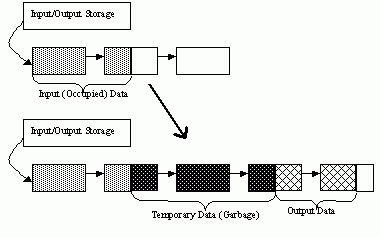
\includegraphics[width=0.5\textwidth]{pics/memstorage1.png}

That is, garbage appears in the middle of the storage. However, if
one creates a child memory storage in the beginning of the processing,
writes temporary data there and releases the child storage in the end,
no garbage will appear in the source/destination storage:

Dynamic data processing using a child storage

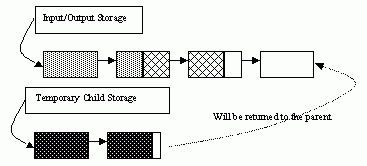
\includegraphics[width=0.5\textwidth]{pics/memstorage2.png}

\cvfunc{ReleaseMemStorage}\label{ReleaseMemStorage}

Releases memory storage

\cvexp{

void cvReleaseMemStorage( CvMemStorage** storage );

}{CPP}{PYTHON}

\begin{description}
\cvarg{storage}{Pointer to the released storage}
\end{description}

The function \texttt{cvReleaseMemStorage} deallocates all storage memory
blocks or returns them to the parent, if any. Then it deallocates the
storage header and clears the pointer to the storage. All children of
the storage must be released before the parent is released.

\cvfunc{ClearMemStorage}\label{ClearMemStorage}

Clears memory storage

\cvexp{

void cvClearMemStorage( CvMemStorage* storage );

}{CPP}{PYTHON}

\begin{description}
\cvarg{storage}{Memory storage}
\end{description}

The function \texttt{cvClearMemStorage} resets the top (free space
boundary) of the storage to the very beginning. This function does not
deallocate any memory. If the storage has a parent, the function returns
all blocks to the parent.

\cvfunc{MemStorageAlloc}\label{MemStorageAlloc}

Allocates memory buffer in the storage

\cvexp{

void* cvMemStorageAlloc( \par CvMemStorage* storage,\par size\_t size );

}{CPP}{PYTHON}

\begin{description}
\cvarg{storage}{Memory storage}
\cvarg{size}{Buffer size}
\end{description}

The function \texttt{cvMemStorageAlloc} allocates memory buffer in
the storage. The buffer size must not exceed the storage block size,
otherwise runtime error is raised. The buffer address is aligned by
\texttt{CV\_STRUCT\_ALIGN=sizeof(double)} for the moment) bytes.

\cvfunc{MemStorageAllocString}\label{MemStorageAllocString}

Allocates text string in the storage

\cvexp{

CvString cvMemStorageAllocString( CvMemStorage* storage, const char* ptr, int len=-1 );

}{CPP}{PYTHON}

\begin{lstlisting}

typedef struct CvString
{
    int len;
    char* ptr;
}
CvString;

\end{lstlisting}

\begin{description}
\cvarg{storage}{Memory storage}
\cvarg{ptr}{The string}
\cvarg{len}{Length of the string (not counting the ending \texttt{NUL}) . If the parameter is negative, the function computes the length.}
\end{description}

The function \texttt{cvMemStorageAllocString} creates copy of the string
in the memory storage. It returns the structure that contains user-passed
or computed length of the string and pointer to the copied string.

\cvfunc{SaveMemStoragePos}\label{SaveMemStoragePos}

Saves memory storage position

\cvexp{

void cvSaveMemStoragePos( \par const CvMemStorage* storage,\par CvMemStoragePos* pos );

}{CPP}{PYTHON}

\begin{description}
\cvarg{storage}{Memory storage}
\cvarg{pos}{The output position of the storage top}
\end{description}

The function \texttt{cvSaveMemStoragePos} saves the current position
of the storage top to the parameter \texttt{pos}. The function
\texttt{cvRestoreMemStoragePos} can further retrieve this position.

\cvfunc{RestoreMemStoragePos}\label{RestoreMemStoragePos}

Restores memory storage position

\cvexp{

void cvRestoreMemStoragePos( \par CvMemStorage* storage,\par CvMemStoragePos* pos );

}{CPP}{PYTHON}

\begin{description}
\cvarg{storage}{Memory storage}
\cvarg{pos}{New storage top position}
\end{description}

The function \texttt{cvRestoreMemStoragePos} restores the position of the storage top from the parameter \texttt{pos}. This function and The function \texttt{cvClearMemStorage} are the only methods to release memory occupied in memory blocks. Note again that there is no way to free memory in the middle of the occupied part of the storage.

\subsection{Sequences}

\cvstruct{CvSeq}\label{CvSeq}

Growable sequence of elements

\begin{lstlisting}

#define CVgSEQUENCE\_FIELDS() \
    int flags; /* micsellaneous flags */ \
    int headergsize; /* size of sequence header */ \
    struct CvSeq* hgprev; /* previous sequence */ \
    struct CvSeq* hgnext; /* next sequence */ \
    struct CvSeq* vgprev; /* 2nd previous sequence */ \
    struct CvSeq* vgnext; /* 2nd next sequence */ \
    int total; /* total number of elements */ \
    int elemgsize;/* size of sequence element in bytes */ \
    char* blockgmax;/* maximal bound of the last block */ \
    char* ptr; /* current write pointer */ \
    int deltagelems; /* how many elements allocated when the sequence grows (sequence granularity) */ \
    CvMemStorage* storage; /* where the seq is stored */ \
    CvSeqBlock* freegblocks; /* free blocks list */ \
    CvSeqBlock* first; /* pointer to the first sequence block */

typedef struct CvSeq
{
    CVgSEQUENCE\_FIELDS()
} CvSeq;

\end{lstlisting}

The structure \cross{CvSeq} is a base for all of OpenCV dynamic data structures.

Such an unusual definition via a helper macro simplifies the extension
of the structure \cross{CvSeq} with additional parameters. To extend
\cross{CvSeq} the user may define a new structure and put user-defined
fields after all \cross{CvSeq} fields that are included via the macro
\texttt{CV\_SEQUENCE\_FIELDS()}.

There are two types of sequences - dense and sparse. Base type for dense
sequences is \cross{CvSeq} and such sequences are used to represent
growable 1d arrays - vectors, stacks, queues, deques. They have no gaps
in the middle - if an element is removed from the middle or inserted
into the middle of the sequence the elements from the closer end are
shifted. Sparse sequences have \cross{CvSet} base class and they are
discussed later in more details. They are sequences of nodes each of
those may be either occupied or free as indicated by the node flag. Such
sequences are used for unordered data structures such as sets of elements,
graphs, hash tables etc.

The field \texttt{header\_size} contains the actual size of the sequence
header and should be greater or equal to \texttt{sizeof(CvSeq)}.

The fields
\texttt{h\_prev}, \texttt{h\_next}, \texttt{v\_prev}, \texttt{v\_next}
can be used to create hierarchical structures from separate sequences. The
fields \texttt{h\_prev} and \texttt{h\_next} point to the previous and
the next sequences on the same hierarchical level while the fields
\texttt{v\_prev} and \texttt{v\_next} point to the previous and the
next sequence in the vertical direction, that is, parent and its first
child. But these are just names and the pointers can be used in a
different way.

The field \texttt{first} points to the first sequence block, whose structure is described below.

The field \texttt{total} contains the actual number of dense sequence elements and number of allocated nodes in sparse sequence.

The field \texttt{flags}contain the particular dynamic type
signature (\texttt{CV\_SEQ\_MAGIC\_VAL} for dense sequences and
\texttt{CV\_SET\_MAGIC\_VAL} for sparse sequences) in the highest 16
bits and miscellaneous information about the sequence. The lowest
\texttt{CV\_SEQ\_ELTYPE\_BITS} bits contain the ID of the element
type. Most of sequence processing functions do not use element type but
element size stored in \texttt{elem\_size}. If sequence contains the
numeric data of one of \cross{CvMat} type then the element type matches
to the corresponding \cross{CvMat} element type, e.g. \texttt{CV\_32SC2} may be
used for sequence of 2D points, \texttt{CV\_32FC1} for sequences of floating-point
values etc. \texttt{CV\_SEQ\_ELTYPE(seq\_header\_ptr)} macro retrieves the
type of sequence elements. Processing function that work with numerical
sequences check that \texttt{elem\_size} is equal to the calculated from
the type element size. Besides \cross{CvMat} compatible types, there
are few extra element types defined in \texttt{cvtypes.h} header:

Standard Types of Sequence Elements

\begin{lstlisting}

#define CV_SEQ_ELTYPE_POINT          CV_32SC2  /* (x,y) */
#define CV_SEQ_ELTYPE_CODE           CV_8UC1   /* freeman code: 0..7 */
#define CV_SEQ_ELTYPE_GENERIC        0 /* unspecified type of sequence elements */
#define CV_SEQ_ELTYPE_PTR            CV_USRTYPE1 /* =6 */
#define CV_SEQ_ELTYPE_PPOINT         CV_SEQ_ELTYPE_PTR  /* &elem: pointer to element of other sequence */
#define CV_SEQ_ELTYPE_INDEX          CV_32SC1  /* #elem: index of element of some other sequence */
#define CV_SEQ_ELTYPE_GRAPH_EDGE     CV_SEQ_ELTYPE_GENERIC  /* &next_o, &next_d, &vtx_o, &vtx_d */
#define CV_SEQ_ELTYPE_GRAPH_VERTEX   CV_SEQ_ELTYPE_GENERIC  /* first_edge, &(x,y) */
#define CV_SEQ_ELTYPE_TRIAN_ATR      CV_SEQ_ELTYPE_GENERIC  /* vertex of the binary tree   */
#define CV_SEQ_ELTYPE_CONNECTED_COMP CV_SEQ_ELTYPE_GENERIC  /* connected component  */
#define CV_SEQ_ELTYPE_POINT3D        CV_32FC3  /* (x,y,z)  */

\end{lstlisting}

The next \texttt{CV\_SEQ\_KIND\_BITS} bits specify the kind of the sequence:

Standard Kinds of Sequences

\begin{lstlisting}

/* generic (unspecified) kind of sequence */
#define CV_SEQ_KIND_GENERIC     (0 << CV_SEQ_ELTYPE_BITS)

/* dense sequence suntypes */
#define CV_SEQ_KIND_CURVE       (1 << CV_SEQ_ELTYPE_BITS)
#define CV_SEQ_KIND_BIN_TREE    (2 << CV_SEQ_ELTYPE_BITS)

/* sparse sequence (or set) subtypes */
#define CV_SEQ_KIND_GRAPH       (3 << CV_SEQ_ELTYPE_BITS)
#define CV_SEQ_KIND_SUBDIV2D    (4 << CV_SEQ_ELTYPE_BITS)

\end{lstlisting}

The remaining bits are used to identify different features specific
to certain sequence kinds and element types. For example, curves
made of points ( \texttt{CV\_SEQ\_KIND\_CURVE|CV\_SEQ\_ELTYPE\_POINT} ),
together with the flag \texttt{CV\_SEQ\_FLAG\_CLOSED} belong to the
type \texttt{CV\_SEQ\_POLYGON} or, if other flags are used, to its
subtype. Many contour processing functions check the type of the input
sequence and report an error if they do not support this type. The
file \texttt{cvtypes.h} stores the complete list of all supported
predefined sequence types and helper macros designed to get the sequence
type of other properties. Below follows the definition of the building
block of sequences.

\cvstruct{CvSeqBlock}\label{CvSeqBlock}

Continuous sequence block

\begin{lstlisting}

typedef struct CvSeqBlock
{
    struct CvSeqBlock* prev; /* previous sequence block */
    struct CvSeqBlock* next; /* next sequence block */
    int start_index; /* index of the first element in the block +
    sequence->first->start_index */
    int count; /* number of elements in the block */
    char* data; /* pointer to the first element of the block */
} CvSeqBlock;

\end{lstlisting}

Sequence blocks make up a circular double-linked list, so the pointers
\texttt{prev} and \texttt{next} are never \texttt{NULL} and point to the
previous and the next sequence blocks within the sequence. It means that
\texttt{next} of the last block is the first block and \texttt{prev} of
the first block is the last block. The fields \texttt{start\_index} and
\texttt{count} help to track the block location within the sequence. For
example, if the sequence consists of 10 elements and splits into three
blocks of 3, 5, and 2 elements, and the first block has the parameter
\texttt{start\_index = 2}, then pairs \texttt{(start\_index, count)} for the sequence
blocks are
(2,3), (5, 5), and (10, 2)
correspondingly. The parameter
\texttt{start\_index} of the first block is usually \texttt{0} unless
some elements have been inserted at the beginning of the sequence.

\cvstruct{CvSlice}\label{CvSlice}

A sequence slice

\begin{lstlisting}

typedef struct CvSlice
{
    int start_index;
    int end_index;
} CvSlice;

inline CvSlice cvSlice( int start, int end );
#define CV_WHOLE_SEQ_END_INDEX 0x3fffffff
#define CV_WHOLE_SEQ  cvSlice(0, CV_WHOLE_SEQ_END_INDEX)

/* calculates the sequence slice length */
int cvSliceLength( CvSlice slice, const CvSeq* seq );

\end{lstlisting}

Some of functions that operate on sequences take \texttt{CvSlice slice}
parameter that is often set to the whole sequence (CV\_WHOLE\_SEQ) by
default. Either of the \texttt{start\_index} and \texttt{end\_index}
may be negative or exceed the sequence length, \texttt{start\_index} is
inclusive, \texttt{end\_index} is exclusive boundary. If they are equal,
the slice is considered empty (i.e. contains no elements). Because
sequences are treated as circular structures, the slice may select a
few elements in the end of a sequence followed by a few elements in the
beginning of the sequence, for example, \texttt{cvSlice(-2, 3)} in case of
10-element sequence will select 5-element slice, containing pre-last
(8th), last (9th), the very first (0th), second (1th) and third (2nd)
elements. The functions normalize the slice argument in the following way:
first, \cross{SliceLength} is called to determine the length of the slice,
then, \texttt{start\_index} of the slice is normalized similarly to the
argument of \cross{GetSeqElem} (i.e. negative indices are allowed). The
actual slice to process starts at the normalized \texttt{start\_index}
and lasts \cross{SliceLength} elements (again, assuming the sequence is
a circular structure).

If a function does not take slice argument, but you want to process
only a part of the sequence, the sub-sequence may be extracted
using \cross{SeqSlice} function, or stored as into a continuous
buffer with \cross{CvtSeqToArray} (optionally, followed by
\cross{MakeSeqHeaderForArray}.

\cvfunc{CreateSeq}\label{CreateSeq}

Creates sequence

\cvexp{

CvSeq* cvCreateSeq( \par int seq\_flags,\par int header\_size,\par int elem\_size,\par CvMemStorage* storage );

}{CPP}{PYTHON}

\begin{description}
\cvarg{seq\_flags}{Flags of the created sequence. If the sequence is not passed to any function working with a specific type of sequences, the sequence value may be set to 0, otherwise the appropriate type must be selected from the list of predefined sequence types.}
\cvarg{header\_size}{Size of the sequence header; must be greater or equal to \texttt{sizeof(CvSeq)}. If a specific type or its extension is indicated, this type must fit the base type header.}
\cvarg{elem\_size}{Size of the sequence elements in bytes. The size must be consistent with the sequence type. For example, for a sequence of points to be created, the element type \texttt{CV\_SEQ\_ELTYPE\_POINT} should be specified and the parameter \texttt{elem\_size} must be equal to \texttt{sizeof(CvPoint)}}
\cvarg{storage}{Sequence location}
\end{description}

The function \texttt{cvCreateSeq} creates a sequence and returns
the pointer to it. The function allocates the sequence header in
the storage block as one continuous chunk and sets the structure
fields \texttt{flags}, \texttt{elem\_size}, \texttt{header\_size} and
\texttt{storage} to passed values, sets \texttt{delta\_elems} to the
default value (that may be reassigned using \cross{SetSeqBlockSize}
function), and clears other header fields, including the space after
the first \texttt{sizeof(CvSeq)} bytes.

\cvfunc{SetSeqBlockSize}\label{SetSeqBlockSize}

Sets up sequence block size

\cvexp{

void cvSetSeqBlockSize( \par CvSeq* seq,\par int delta\_elems );

}{CPP}{PYTHON}

\begin{description}
\cvarg{seq}{Sequence}
\cvarg{delta\_elems}{Desirable sequence block size in elements}
\end{description}


The function \texttt{cvSetSeqBlockSize} affects memory allocation
granularity. When the free space in the sequence buffers has run out,
the function allocates the space for \texttt{delta\_elems} sequence
elements. If this block immediately follows the one previously allocated,
the two blocks are concatenated, otherwise, a new sequence block is
created. Therefore, the bigger the parameter is, the lower the possible
sequence fragmentation, but the more space in the storage is wasted. When
the sequence is created, the parameter \texttt{delta\_elems} is set to
the default value  about 1K. The function can be called any time after
the sequence is created and affects future allocations. The function
can modify the passed value of the parameter to meet the memory storage
constraints.

\cvfunc{SeqPush}\label{SeqPush}

Adds element to sequence end

\cvexp{

char* cvSeqPush( \par CvSeq* seq,\par void* element=NULL );

}{CPP}{PYTHON}

\begin{description}
\cvarg{seq}{Sequence}
\cvarg{element}{Added element}
\end{description}


The function \texttt{cvSeqPush} adds an element to the end of sequence and retuns pointer to the allocated element. If the input \texttt{element} is NULL, the function simply allocates a space for one more element.

The following code demonstrates how to create a new sequence using this function:

\begin{lstlisting}

CvMemStorage* storage = cvCreateMemStorage(0);
CvSeq* seq = cvCreateSeq( CV_32SC1, /* sequence of integer elements */
                          sizeof(CvSeq), /* header size - no extra fields */
                          sizeof(int), /* element size */
                          storage /* the container storage */ );
int i;
for( i = 0; i < 100; i++ )
{
    int* added = (int*)cvSeqPush( seq, &i );
    printf( "%d is added\n", *added );
}

...
/* release memory storage in the end */
cvReleaseMemStorage( &storage );

\end{lstlisting}

The function \texttt{cvSeqPush} has O(1) complexity, but there is a faster method for writing large sequences (see \cross{StartWriteSeq} and related functions).


\cvfunc{SeqPop}\label{SeqPop}

Removes element from sequence end

\cvexp{

void cvSeqPop( \par CvSeq* seq,\par void* element=NULL );

}{CPP}{PYTHON}

\begin{description}
\cvarg{seq}{Sequence}
\cvarg{element}{Optional parameter . If the pointer is not zero, the function copies the removed element to this location.}
\end{description}

The function \texttt{cvSeqPop} removes an element from the sequence. The function reports an error if the sequence is already empty. The function has O(1) complexity.

\cvfunc{SeqPushFront}\label{SeqPushFront}

Adds element to sequence beginning

\cvexp{

char* cvSeqPushFront( CvSeq* seq, void* element=NULL );

}{CPP}{PYTHON}

\begin{description}
\cvarg{seq}{Sequence}
\cvarg{element}{Added element}
\end{description}

The function \texttt{cvSeqPushFront} is similar to \cross{SeqPush} but it adds the new element to the beginning of the sequence. The function has O(1) complexity.

\cvfunc{SeqPopFront}\label{SeqPopFront}

Removes element from sequence beginning

\cvexp{

void cvSeqPopFront( \par \par CvSeq* seq,\par\par void* element=NULL );

}{CPP}{PYTHON}

\begin{description}
\cvarg{seq}{Sequence}
\cvarg{element}{Optional parameter. If the pointer is not zero, the function copies the removed element to this location.}
\end{description}

The function \texttt{cvSeqPopFront} removes an element from the beginning of the sequence. The function reports an error if the sequence is already empty. The function has O(1) complexity.

\cvfunc{SeqPushMulti}\label{SeqPushMulti}

Pushes several elements to the either end of sequence

\cvexp{

void cvSeqPushMulti( \par CvSeq* seq,\par void* elements,\par int count,\par int in\_front=0 );

}{CPP}{PYTHON}

\begin{description}
\cvarg{seq}{Sequence}
\cvarg{elements}{Added elements}
\cvarg{count}{Number of elements to push}
\cvarg{in\_front}{The flags specifying the modified sequence end
\begin{description}
\cvarg{CV\_BACK}{the elements are added to the end of sequence}
\cvarg{CV\_FRONT}{the elements are added to the beginning of sequence}
\end{description}}
\end{description}

The function \texttt{cvSeqPushMulti} adds several elements to either
end of the sequence. The elements are added to the sequence in the same
order as they are arranged in the input array but they can fall into
different sequence blocks.

\cvfunc{SeqPopMulti}\label{SeqPopMulti}

Removes several elements from the either end of sequence

\cvexp{

void cvSeqPopMulti( \par CvSeq* seq,\par void* elements,\par int count,\par int in\_front=0 );

}{CPP}{PYTHON}

\begin{description}
\cvarg{seq}{Sequence}
\cvarg{elements}{Removed elements}
\cvarg{count}{Number of elements to pop}
\cvarg{in\_front}{The flags specifying the modified sequence end
\begin{description}
\cvarg{CV\_BACK}{the elements are added to the end of sequence}
\cvarg{CV\_FRONT}{the elements are added to the beginning of sequence}
\end{description}}
\end{description}

The function \texttt{cvSeqPopMulti} removes several elements from either end of the sequence. If the number of the elements to be removed exceeds the total number of elements in the sequence, the function removes as many elements as possible.

\cvfunc{SeqInsert}\label{SeqInsert}

Inserts element in sequence middle

\cvexp{

char* cvSeqInsert( \par CvSeq* seq,\par int before\_index,\par void* element=NULL );

}{CPP}{PYTHON}

\begin{description}
\cvarg{seq}{Sequence}
\cvarg{before\_index}{Index before which the element is inserted. Inserting before 0 (the minimal allowed value of the parameter) is equal to \cross{SeqPushFront} and inserting before \texttt{seq->total} (the maximal allowed value of the parameter) is equal to \cross{SeqPush}.}
\cvarg{element}{Inserted element} 
\end{description}

The function \texttt{cvSeqInsert} shifts the sequence elements from the inserted position to the nearest end of the sequence and copies the \texttt{element} content there if the pointer is not NULL. The function returns pointer to the inserted element.

\cvfunc{SeqRemove}\label{SeqRemove}

Removes element from sequence middle

\cvexp{

void cvSeqRemove( \par CvSeq* seq,\par int index );

}{CPP}{SeqRemove(seq,index)-> None}

\begin{description}
\cvarg{seq}{Sequence}
\cvarg{index}{Index of removed element}
\end{description}


The function \texttt{cvSeqRemove} removes elements with the given
index. If the index is out of range the function reports an error. An
attempt to remove an element from an empty sequence is a partitial
case of this situation. The function removes an element by shifting
the sequence elements between the nearest end of the sequence and the
\texttt{index}-th position, not counting the latter.


\cvfunc{ClearSeq}\label{ClearSeq}

Clears sequence

\cvexp{

void cvClearSeq( CvSeq* seq );

}{CPP}{ClearSeq(seq)-> None}

\begin{description}
\cvarg{seq}{Sequence}
\end{description}


The function \texttt{cvClearSeq} removes all elements from the
sequence. The function does not return the memory to the storage, but this
memory is reused later when new elements are added to the sequence. This
function time complexity is 'O(1)'.

\cvfunc{GetSeqElem}\label{GetSeqElem}

Returns pointer to sequence element by its index

\cvexp{

char* cvGetSeqElem( const CvSeq* seq, int index );

}{CPP}{PYTHON}

\begin{lstlisting}
#define CV_GET_SEQ_ELEM( TYPE, seq, index )  (TYPE*)cvGetSeqElem( (CvSeq*)(seq), (index) )
\end{lstlisting}

\begin{description}
\cvarg{seq}{Sequence}
\cvarg{index}{Index of element}
\end{description}


The function \texttt{cvGetSeqElem} finds the element with the given
index in the sequence and returns the pointer to it. If the element
is not found, the function returns 0. The function supports negative
indices, where -1 stands for the last sequence element, -2 stands for
the one before last, etc. If the sequence is most likely to consist of
a single sequence block or the desired element is likely to be located
in the first block, then the macro
\texttt{CV\_GET\_SEQ\_ELEM( elemType, seq, index )}
should be used, where the parameter \texttt{elemType} is the
type of sequence elements ( \cross{CvPoint} for example), the parameter
\texttt{seq} is a sequence, and the parameter \texttt{index} is the index
of the desired element. The macro checks first whether the desired element
belongs to the first block of the sequence and returns it if it does,
otherwise the macro calls the main function \texttt{GetSeqElem}. Negative
indices always cause the \cross{GetSeqElem} call. The function has O(1)
time complexity assuming that number of blocks is much smaller than the
number of elements.

\cvfunc{SeqElemIdx}\label{SeqElemIdx}

Returns index of concrete sequence element

\cvexp{

int cvSeqElemIdx( \par const CvSeq* seq,\par const void* element,\par CvSeqBlock** block=NULL );

}{CPP}{PYTHON}

\begin{description}
\cvarg{seq}{Sequence}
\cvarg{element}{Pointer to the element within the sequence}
\cvarg{block}{Optional argument. If the pointer is not \texttt{NULL}, the address of the sequence block that contains the element is stored in this location.}
\end{description}

The function \texttt{cvSeqElemIdx} returns the index of a sequence element or a negative number if the element is not found.

\cvfunc{CvtSeqToArray}\label{CvtSeqToArray}

Copies sequence to one continuous block of memory

\cvexp{

void* cvCvtSeqToArray( \par const CvSeq* seq,\par void* elements,\par CvSlice slice=CV\_WHOLE\_SEQ );

}{CPP}{PYTHON}

\begin{description}
\cvarg{seq}{Sequence}
\cvarg{elements}{Pointer to the destination array that must be large enough. It should be a pointer to data, not a matrix header.}
\cvarg{slice}{The sequence part to copy to the array}
\end{description}


The function \texttt{cvCvtSeqToArray} copies the entire sequence or subsequence to the specified buffer and returns the pointer to the buffer.


\cvfunc{MakeSeqHeaderForArray}\label{MakeSeqHeaderForArray}

Constructs sequence from array

\cvexp{

CvSeq* cvMakeSeqHeaderForArray( \par int seq\_type,\par int header\_size,\par int elem\_size,\par void* elements,\par int total,\par CvSeq* seq,\par CvSeqBlock* block );

}{CPP}{PYTHON}

\begin{description}
\cvarg{seq\_type}{Type of the created sequence}
\cvarg{header\_size}{Size of the header of the sequence . Parameter sequence must point to the structure of that size or greater size.}
\cvarg{elem\_size}{Size of the sequence element}
\cvarg{elements}{Elements that will form a sequence}
\cvarg{total}{Total number of elements in the sequence. The number of array elements must be equal to the value of this parameter.}
\cvarg{seq}{Pointer to the local variable that is used as the sequence header}
\cvarg{block}{Pointer to the local variable that is the header of the single sequence block}
\end{description}

The function \texttt{cvMakeSeqHeaderForArray} initializes sequence
header for array. The sequence header as well as the sequence block are
allocated by the user (for example, on stack). No data is copied by the
function. The resultant sequence will consists of a single block and
have NULL storage pointer, thus, it is possible to read its elements,
but the attempts to add elements to the sequence will raise an error in
most cases.

\cvfunc{SeqSlice}\label{SeqSlice}

Makes separate header for the sequence slice

\cvexp{

CvSeq* cvSeqSlice( \par const CvSeq* seq,\par CvSlice slice,\par CvMemStorage* storage=NULL,\par int copy\_data=0 );

}{CPP}{PYTHON}

\begin{description}
\cvarg{seq}{Sequence}
\cvarg{slice}{The part of the sequence to extract}
\cvarg{storage}{The destination storage to keep the new sequence header and the copied data if any . If it is NULL, the function uses the storage containing the input sequence.}
\cvarg{copy\_data}{The flag that indicates whether to copy the elements of the extracted slice (\texttt{copy\_data!=0}) or not (\texttt{copy\_data=0})}
\end{description}

The function \texttt{cvSeqSlice} creates a sequence that represents the specified slice of the input sequence. The new sequence either shares the elements with the original sequence or has own copy of the elements. So if one needs to process a part of sequence but the processing function does not have a slice parameter, the required sub-sequence may be extracted using this function.


\cvfunc{CloneSeq}\label{CloneSeq}

Creates a copy of sequence

\cvexp{

CvSeq* cvCloneSeq( \par const CvSeq* seq,\par CvMemStorage* storage=NULL );

}{CPP}{CloneSeq(seq,storage)-> None}

\begin{description}
\cvarg{seq}{Sequence}
\cvarg{storage}{The destination storage to keep the new sequence header and the copied data if any. If it is NULL, the function uses the storage containing the input sequence.} 
\end{description}

The function \texttt{cvCloneSeq} makes a complete copy of the input sequence and returns it. The call

\begin{lstlisting}
cvCloneSeq( seq, storage )
\end{lstlisting}

is equivalent to

\begin{lstlisting}
cvSeqSlice]( seq, CV\_WHOLE\_SEQ, storage, 1 )
\end{lstlisting}

\cvfunc{SeqRemoveSlice}\label{SeqRemoveSlice}

Removes sequence slice

\cvexp{

void cvSeqRemoveSlice( CvSeq* seq, CvSlice slice );

}{CPP}{SeqRemoveSlice(seq,slice)-> None}

\begin{description}
\cvarg{seq}{Sequence}
\cvarg{slice}{The part of the sequence to remove}
\end{description}


The function \texttt{cvSeqRemoveSlice} removes slice from the sequence.

\cvfunc{SeqInsertSlice}\label{SeqInsertSlice}

Inserts array in the middle of sequence

\cvexp{

void cvSeqInsertSlice( \par CvSeq* seq,\par int before\_index,\par const CvArr* from\_arr );

}{CPP}{PYTHON}

\begin{description}
\cvarg{seq}{Sequence}
\cvarg{slice}{The part of the sequence to remove}
\cvarg{from\_arr}{The array to take elements from}
\end{description}


The function \texttt{cvSeqInsertSlice} inserts all \texttt{from\_arr}
array elements at the specified position of the sequence. The array
\texttt{from\_arr} can be a matrix or another sequence.

\cvfunc{SeqInvert}\label{SeqInvert}

Reverses the order of sequence elements

\cvexp{

void cvSeqInvert( CvSeq* seq );

}{CPP}{SeqInvert(seq)-> None}

\begin{description}
\cvarg{seq}{Sequence}
\end{description}


The function \texttt{cvSeqInvert} reverses the sequence in-place - makes the first element go last, the last element go first etc.


\cvfunc{SeqSort}\label{SeqSort}

Sorts sequence element using the specified comparison function

\cvexp{

void cvSeqSort( CvSeq* seq, CvCmpFunc func, void* userdata=NULL );

}{CPP}{PYTHON}

\begin{lstlisting}
/* a < b ? -1 : a > b ? 1 : 0 */
typedef int (CV_CDECL* CvCmpFunc)(const void* a, const void* b, void* userdata);
\end{lstlisting}

\begin{description}
\cvarg{seq}{The sequence to sort}
\cvarg{func}{The comparison function that returns negative, zero or positive value depending on the elements relation (see the above declaration and the example below) - similar function is used by \texttt{qsort} from C runline except that in the latter \texttt{userdata} is not used}
\cvarg{userdata}{The user parameter passed to the compasion function; helps to avoid global variables in some cases}
\end{description}

The function \texttt{cvSeqSort} sorts the sequence in-place using the specified criteria. Below is the example of the function use:

\begin{lstlisting}

/* Sort 2d points in top-to-bottom left-to-right order */
static int cmp_func( const void* _a, const void* _b, void* userdata )
{
    CvPoint* a = (CvPoint*)_a;
    CvPoint* b = (CvPoint*)_b;
    int y_diff = a->y - b->y;
    int x_diff = a->x - b->x;
    return y_diff ? y_diff : x_diff;
}

...

CvMemStorage* storage = cvCreateMemStorage(0);
CvSeq* seq = cvCreateSeq( CV_32SC2, sizeof(CvSeq), sizeof(CvPoint), storage );
int i;

for( i = 0; i < 10; i++ )
{
    CvPoint pt;
    pt.x = rand() % 1000;
    pt.y = rand() % 1000;
    cvSeqPush( seq, &pt );
}

cvSeqSort( seq, cmp_func, 0 /* userdata is not used here */ );

/* print out the sorted sequence */
for( i = 0; i < seq->total; i++ )
{
    CvPoint* pt = (CvPoint*)cvSeqElem( seq, i );
    printf( "(%d,%d)\n", pt->x, pt->y );
}

cvReleaseMemStorage( &storage );

\end{lstlisting}


\cvfunc{SeqSearch}\label{SeqSearch}

Searches element in sequence

\begin{lstlisting}

/* a < b ? -1 : a > b ? 1 : 0 */
typedef int (CV_CDECL* CvCmpFunc)(const void* a, const void* b, void* userdata);

char* cvSeqSearch( CvSeq* seq, const void* elem, CvCmpFunc func,
                   int is_sorted, int* elem_idx, void* userdata=NULL );

\end{lstlisting}

\begin{description}
\cvarg{seq}{The sequence}
\cvarg{elem}{The element to look for}
\cvarg{func}{The comparison function that returns negative, zero or positive value depending on the elements relation (see also \cross{SeqSort})}
\cvarg{is\_sorted}{Whether the sequence is sorted or not}
\cvarg{elem\_idx}{Output parameter; index of the found element}
\cvarg{userdata}{The user parameter passed to the compasion function; helps to avoid global variables in some cases}
\end{description}

The function \texttt{cvSeqSearch} searches the element in the sequence. If
the sequence is sorted, binary O(log(N)) search is used, otherwise, a
simple linear search is used. If the element is not found, the function
returns NULL pointer and the index is set to the number of sequence
elements if the linear search is used, and to the smallest index
\texttt{i, seq(i)>elem}
.

\cvfunc{StartAppendToSeq}\label{StartAppendToSeq}

Initializes process of writing data to sequence

\cvexp{

void cvStartAppendToSeq( \par CvSeq* seq,\par CvSeqWriter* writer );

}{CPP}{PYTHON}

\begin{description}
\cvarg{seq}{Pointer to the sequence}
\cvarg{writer}{Writer state; initialized by the function}
\end{description}

The function \texttt{cvStartAppendToSeq} initializes the process of
writing data to the sequence. Written elements are added to the end of the
sequence by
\texttt{CV\_WRITE\_SEQ\_ELEM( written\_elem, writer )}
macro. Note
that during the writing process other operations on the sequence may
yield incorrect result or even corrupt the sequence (see description of
\cross{FlushSeqWriter} that helps to avoid some of these problems).

\cvfunc{StartWriteSeq}\label{StartWriteSeq}

Creates new sequence and initializes writer for it

\cvexp{

void cvStartWriteSeq( \par int seq\_flags,\par int header\_size,\par int elem\_size,\par CvMemStorage* storage,\par CvSeqWriter* writer );

}{CPP}{PYTHON}

\begin{description}
\cvarg{seq\_flags}{Flags of the created sequence. If the sequence is not passed to any function working with a specific type of sequences, the sequence value may be equal to 0, otherwise the appropriate type must be selected from the list of predefined sequence types.}
\cvarg{header\_size}{Size of the sequence header. The parameter value may not be less than \texttt{sizeof(CvSeq)}. If a certain type or extension is specified, it must fit the base type header.}
\cvarg{elem\_size}{Size of the sequence elements in bytes; must be consistent with the sequence type. For example, if the sequence of points is created (element type \texttt{CV\_SEQ\_ELTYPE\_POINT} ), then the parameter elem\_size must be equal to \texttt{sizeof(CvPoint)}}
\cvarg{storage}{Sequence location}
\cvarg{writer}{Writer state; initialized by the function}
\end{description}

The function \texttt{cvStartWriteSeq} is a composition of
\cross{CreateSeq} and \cross{StartAppendToSeq}. The pointer to the
created sequence is stored at
\texttt{writer->seq}
and is also returned by
\cross{EndWriteSeq} function that should be called in the end.

\cvfunc{EndWriteSeq}\label{EndWriteSeq}

Finishes process of writing sequence

\cvexp{

CvSeq* cvEndWriteSeq( CvSeqWriter* writer );

}{CPP}{PYTHON}

\begin{description}
\cvarg{writer}{Writer state}
\end{description}


The function \texttt{cvEndWriteSeq} finishes the writing process and
returns the pointer to the written sequence. The function also truncates
the last incomplete sequence block to return the remaining part of the
block to the memory storage. After that the sequence can be read and
modified safely.

\cvfunc{FlushSeqWriter}\label{FlushSeqWriter}

Updates sequence headers from the writer state

\cvexp{

void cvFlushSeqWriter( CvSeqWriter* writer );

}{CPP}{PYTHON}

\begin{description}
\cvarg{writer}{Writer state}
\end{description}

The function \texttt{cvFlushSeqWriter} is intended to enable the user to
read sequence elements, whenever required, during the writing process,
e.g., in order to check specific conditions. The function updates the
sequence headers to make reading from the sequence possible. The writer
is not closed, however, so that the writing process can be continued
any time. In some algorithm requires often flush'es, consider using
\cross{SeqPush} instead.

\cvfunc{StartReadSeq}\label{StartReadSeq}

Initializes process of sequential reading from sequence

\cvexp{

void cvStartReadSeq( \par const CvSeq* seq,\par CvSeqReader* reader,\par int reverse=0 );

}{CPP}{PYTHON}

\begin{description}
\cvarg{seq}{Sequence}
\cvarg{reader}{Reader state; initialized by the function}
\cvarg{reverse}{Determines the direction of the sequence traversal. If \texttt{reverse} is 0, the reader is positioned at the first sequence element, otherwise it is positioned at the last element. }
\end{description}

The function \texttt{cvStartReadSeq} initializes the reader state. After
that all the sequence elements from the first down to the last one
can be read by subsequent calls of the macro
\texttt{CV\_READ\_SEQ\_ELEM( read\_elem, reader )}
in case of forward reading and by using
\texttt{CV\_REV\_READ\_SEQ\_ELEM( read\_elem, reader )}
in case of reversed
reading. Both macros put the sequence element to \texttt{read\_elem} and
move the reading pointer toward the next element. A circular structure
of sequence blocks is used for the reading process, that is, after the
last element has been read by the macro \texttt{CV\_READ\_SEQ\_ELEM}, the
first element is read when the macro is called again. The same applies to
\texttt{CV\_REV\_READ\_SEQ\_ELEM}. There is no function to finish the reading
process, since it neither changes the sequence nor creates any temporary
buffers. The reader field \texttt{ptr} points to the current element of
the sequence that is to be read next. The code below demonstrates how
to use sequence writer and reader.

\begin{lstlisting}

CvMemStorage* storage = cvCreateMemStorage(0);
CvSeq* seq = cvCreateSeq( CV_32SC1, sizeof(CvSeq), sizeof(int), storage );
CvSeqWriter writer;
CvSeqReader reader;
int i;

cvStartAppendToSeq( seq, &writer );
for( i = 0; i < 10; i++ )
{
    int val = rand()%100;
    CV_WRITE_SEQ_ELEM( val, writer );
    printf("%d is written\n", val );
}
cvEndWriteSeq( &writer );

cvStartReadSeq( seq, &reader, 0 );
for( i = 0; i < seq->total; i++ )
{
    int val;
#if 1
    CV_READ_SEQ_ELEM( val, reader );
    printf("%d is read\n", val );
#else /* alternative way, that is prefferable if sequence elements are large,
         or their size/type is unknown at compile time */
    printf("%d is read\n", *(int*)reader.ptr );
    CV_NEXT_SEQ_ELEM( seq->elem_size, reader );
#endif
}
...

cvReleaseStorage( &storage );

\end{lstlisting}

\cvfunc{GetSeqReaderPos}\label{GetSeqReaderPos}

Returns the current reader position

\cvexp{

int cvGetSeqReaderPos( CvSeqReader* reader );

}{CPP}{PYTHON}

\begin{description}
\cvarg{reader}{Reader state}
\end{description}


The function \texttt{cvGetSeqReaderPos} returns the current reader position (within 0 ... \texttt{reader->seq->total} - 1).

\cvfunc{SetSeqReaderPos}\label{SetSeqReaderPos}

Moves the reader to specified position

\cvexp{

void cvSetSeqReaderPos( \par CvSeqReader* reader,\par int index,\par int is\_relative=0 );

}{CPP}{PYTHON}

\begin{description}
\cvarg{reader}{Reader state}
\cvarg{index}{The destination position. If the positioning mode is used (see the next parameter) the actual position will be \texttt{index} mod \texttt{reader->seq->total}.}
\cvarg{is\_relative}{If it is not zero, then \texttt{index} is a relative to the current position}
\end{description}

The function \texttt{cvSetSeqReaderPos} moves the read position to the absolute position or relative to the current position.

\subsection{Sets}

\cvstruct{CvSet}\label{CvSet}

Collection of nodes

\begin{lstlisting}

typedef struct CvSetElem
{
    int flags; /* it is negative if the node is free and zero or positive otherwise */
    struct CvSetElem* next_free; /* if the node is free, the field is a
                                    pointer to next free node */
}
CvSetElem;

#define CV_SET_FIELDS()    \
    CV_SEQUENCE_FIELDS()   /* inherits from [#CvSeq CvSeq] */ \
    struct CvSetElem* free_elems; /* list of free nodes */

typedef struct CvSet
{
    CV_SET_FIELDS()
} CvSet;

\end{lstlisting}

The structure \cross{CvSet} is a base for OpenCV sparse data structures.

As follows from the above declaration \cross{CvSet} inherits from
\cross{CvSeq} and it adds \texttt{free\_elems} field it to, which
is a list of free nodes. Every set node, whether free or not, is the
element of the underlying sequence. While there is no restrictions on
elements of dense sequences, the set (and derived structures) elements
must start with integer field and be able to fit CvSetElem structure,
because these two fields (integer followed by the pointer) are required
for organization of node set with the list of free nodes. If a node is
free, \texttt{flags} field is negative (the most-significant bit, or
MSB, of the field is set), and \texttt{next\_free} points to the next
free node (the first free node is referenced by \texttt{free\_elems}
field of \cross{CvSet}). And if a node is occupied, \texttt{flags} field
is positive and contains the node index that may be retrieved using
(\texttt{set\_elem->flags \& CV\_SET\_ELEM\_IDX\_MASK}) expression, the rest of
the node content is determined by the user. In particular, the occupied
nodes are not linked as the free nodes are, so the second field can be
used for such a link as well as for some different purpose. The macro
'CV\_IS\_SET\_ELEM(set\_elem\_ptr)' can be used to determined whether
the specified node is occupied or not.

Initially the set and the list are empty. When a new node is requiested
from the set, it is taken from the list of free nodes, which is updated
then. If the list appears to be empty, a new sequence block is allocated
and all the nodes within the block are joined in the list of free
nodes. Thus, \texttt{total} field of the set is the total number of nodes
both occupied and free. When an occupied node is released, it is added
to the list of free nodes. The node released last will be occupied first.

In OpenCV \cross{CvSet} is used for representing graphs (\cross{CvGraph}),
sparse multi-dimensional arrays (\cross{CvSparseMat}), planar subdivisions
\cross{CvSubdiv2D}.

\cvfunc{CreateSet}\label{CreateSet}

Creates empty set

\cvexp{

CvSet* cvCreateSet( \par int set\_flags,\par int header\_size,\par int elem\_size,\par CvMemStorage* storage );

}{CPP}{PYTHON}

\begin{description}
\cvarg{set\_flags}{Type of the created set}
\cvarg{header\_size}{Set header size; may not be less than \texttt{sizeof(CvSet)}}
\cvarg{elem\_size}{Set element size; may not be less than \cross{CvSetElem}}
\cvarg{storage}{Container for the set}
\end{description}

The function \texttt{cvCreateSet} creates an empty set with a specified header size and element size, and returns the pointer to the set. The function is just a thin layer on top of \cross{CreateSeq}.

\cvfunc{SetAdd}\label{SetAdd}

Occupies a node in the set

\cvexp{

int cvSetAdd( \par CvSet* set\_header,\par CvSetElem* elem=NULL,\par CvSetElem** inserted\_elem=NULL );

}{CPP}{PYTHON}

\begin{description}
\cvarg{set\_header}{Set}
\cvarg{elem}{Optional input argument, inserted element. If not NULL, the function copies the data to the allocated node (The MSB of the first integer field is cleared after copying).}
\cvarg{inserted\_elem}{Optional output argument; the pointer to the allocated cell}
\end{description}

The function \texttt{cvSetAdd} allocates a new node, optionally copies
input element data to it, and returns the pointer and the index to the
node. The index value is taken from the lower bits of \texttt{flags}
field of the node. The function has O(1) complexity, however there exists
a faster function for allocating set nodes (see \cross{SetNew}).

\cvfunc{SetRemove}\label{SetRemove}

Removes element from set

\cvexp{

void cvSetRemove( \par CvSet* set\_header,\par int index );

}{CPP}{PYTHON}

\begin{description}
\cvarg{set\_header}{Set}
\cvarg{index}{Index of the removed element}
\end{description}

The function \texttt{cvSetRemove} removes an element with a specified
index from the set. If the node at the specified location is not occupied
the function does nothing. The function has O(1) complexity, however,
\cross{SetRemoveByPtr} provides yet faster way to remove a set element
if it is located already.

\cvfunc{SetNew}\label{SetNew}

Adds element to set (fast variant)

\cvexp{

CvSetElem* cvSetNew( CvSet* set\_header );

}{CPP}{PYTHON}

\begin{description}
\cvarg{set\_header}{Set}
\end{description}


The function \texttt{cvSetNew} is inline light-weight variant of \cross{SetAdd}. It occupies a new node and returns pointer to it rather than index.


\cvfunc{SetRemoveByPtr}\label{SetRemoveByPtr}

Removes set element given its pointer

\cvexp{

void cvSetRemoveByPtr( \par CvSet* set\_header,\par void* elem );

}{CPP}{PYTHON}

\begin{description}
\cvarg{set\_header}{Set}
\cvarg{elem}{Removed element}
\end{description}

The function \texttt{cvSetRemoveByPtr} is inline light-weight variant of \cross{SetRemove} that takes element pointer. The function does not check whether the node is occupied or not - the user should take care of it.


\cvfunc{GetSetElem}\label{GetSetElem}

Finds set element by its index

\cvexp{

CvSetElem* cvGetSetElem( \par const CvSet* set\_header,\par int index );

}{CPP}{PYTHON}

\begin{description}
\cvarg{set\_header}{Set}
\cvarg{index}{Index of the set element within a sequence}
\end{description}

The function \texttt{cvGetSetElem} finds a set element by index. The function returns the pointer to it or 0 if the index is invalid or the corresponding node is free. The function supports negative indices as it uses \cross{GetSeqElem} to locate the node.

\cvfunc{ClearSet}\label{ClearSet}

Clears set

\cvexp{

void cvClearSet( CvSet* set\_header );

}{CPP}{PYTHON}

\begin{description}
\cvarg{set\_header}{Cleared set}
\end{description}


The function \texttt{cvClearSet} removes all elements from set. It has O(1) time complexity.


\subsection{Graphs}


\cvstruct{CvGraph}\label{CvGraph}

Oriented or unoriented weigted graph

\begin{lstlisting}

#define CV_GRAPH_VERTEX_FIELDS()    \
    int flags; /* vertex flags */   \
    struct CvGraphEdge* first; /* the first incident edge */

typedef struct CvGraphVtx
{
    CV_GRAPH_VERTEX_FIELDS()
}
CvGraphVtx;

#define CV_GRAPH_EDGE_FIELDS()      \
    int flags; /* edge flags */     \
    float weight; /* edge weight */ \
    struct CvGraphEdge* next[2]; /* the next edges in the incidence lists for staring (0) */ \
                                  /* and ending (1) vertices */ \
    struct CvGraphVtx* vtx[2]; /* the starting (0) and ending (1) vertices */

typedef struct CvGraphEdge
{
    CV_GRAPH_EDGE_FIELDS()
}
CvGraphEdge;

#define  CV_GRAPH_FIELDS()                  \
    CV_SET_FIELDS() /* set of vertices */   \
    CvSet* edges;   /* set of edges */

typedef struct CvGraph
{
    CV_GRAPH_FIELDS()
}
CvGraph;

\end{lstlisting}

The structure \cross{CvGraph} is a base for graphs used in OpenCV.

Graph structure inherits from \cross{CvSet} - this part describes common graph properties and the graph vertices, and contains another set as a member - this part describes the graph edges.

The vertex, edge and the graph header structures are declared using the
same technique as other extendible OpenCV structures - via macros, that
simplifies extension and customization of the structures. While the vertex
and edge structures do not inherit from \cross{CvSetElem} explicitly, they
satisfy both conditions on the set elements - have an integer field in
the beginning and fit CvSetElem structure. The \texttt{flags} fields are
used as for indicating occupied vertices and edges as well as for other
purposes, for example, for graph traversal (see \cross{CreateGraphScanner}
et al.), so it is better not to use them directly.

The graph is represented as a set of edges each of whose has the list of
incident edges. The incidence lists for different vertices are interleaved
to avoid information duplication as much as posssible.

The graph may be oriented or unoriented. In the latter case there is no
distiction between edge connecting vertex $A$ with vertex $B$ and the edge
connecting vertex $B$ with vertex $A$ - only one of them can exist in the
graph at the same moment and it represents both $A \rightarrow B$ and
$B \rightarrow A$ edges..

\cvfunc{CreateGraph}\label{CreateGraph}

Creates empty graph

\cvexp{

CvGraph* cvCreateGraph( \par int graph\_flags,\par int header\_size,\par int vtx\_size,\par int edge\_size,\par CvMemStorage* storage );

}{CPP}{PYTHON}

\begin{description}
\cvarg{graph\_flags}{Type of the created graph. Usually, it is either \texttt{CV\_SEQ\_KIND\_GRAPH} for generic unoriented graphs and
\texttt{CV\_SEQ\_KIND\_GRAPH | CV\_GRAPH\_FLAG\_ORIENTED} for generic oriented graphs.}
\cvarg{header\_size}{Graph header size; may not be less than \texttt{sizeof(CvGraph)}}
\cvarg{vtx\_size}{Graph vertex size; the custom vertex structure must start with \cross{CvGraphVtx} (use 'CV\_GRAPH\_VERTEX\_FIELDS()')}
\cvarg{edge\_size}{Graph edge size; the custom edge structure must start with \cross{CvGraphEdge} (use 'CV\_GRAPH\_EDGE\_FIELDS()')}
\cvarg{storage}{The graph container}
\end{description}

The function \texttt{cvCreateGraph} creates an empty graph and returns pointer to it.

\cvfunc{GraphAddVtx}\label{GraphAddVtx}

Adds vertex to graph

\cvexp{

int cvGraphAddVtx( \par CvGraph* graph,\par const CvGraphVtx* vtx=NULL,\par CvGraphVtx** inserted\_vtx=NULL );

}{CPP}{PYTHON}

\begin{description}
\cvarg{graph}{Graph}
\cvarg{vtx}{Optional input argument used to initialize the added vertex (only user-defined fields beyond 'sizeof(CvGraphVtx)' are copied)}
\cvarg{inserted\_vertex}{Optional output argument. If not \texttt{NULL}, the address of the new vertex is written there.}
\end{description}

The function \texttt{cvGraphAddVtx} adds a vertex to the graph and returns the vertex index.

\cvfunc{GraphRemoveVtx}\label{GraphRemoveVtx}

Removes vertex from graph

\cvexp{

int cvGraphRemoveVtx( \par CvGraph* graph,\par int index );

}{CPP}{PYTHON}

\begin{description}
\cvarg{graph}{Graph}
\cvarg{vtx\_idx}{Index of the removed vertex}
\end{description}

The function \texttt{cvGraphRemoveAddVtx} removes a vertex from the graph
together with all the edges incident to it. The function reports an error,
if the input vertex does not belong to the graph. The return value is
number of edges deleted, or -1 if the vertex does not belong to the graph.

\cvfunc{GraphRemoveVtxByPtr}\label{GraphRemoveVtxByPtr}

Removes vertex from graph

\cvexp{

int cvGraphRemoveVtxByPtr( \par CvGraph* graph,\par CvGraphVtx* vtx );

}{CPP}{PYTHON}

\begin{description}
\cvarg{graph}{Graph}
\cvarg{vtx}{Pointer to the removed vertex}
\end{description}


The function \texttt{cvGraphRemoveVtxByPtr} removes a vertex from the graph together with all the edges incident to it. The function reports an error, if the vertex does not belong to the graph. The return value is number of edges deleted, or -1 if the vertex does not belong to the graph.

\cvfunc{GetGraphVtx}\label{GetGraphVtx}

Finds graph vertex by index

\cvexp{

CvGraphVtx* cvGetGraphVtx( \par CvGraph* graph,\par int vtx\_idx );

}{CPP}{PYTHON}

\begin{description}
\cvarg{graph}{Graph}
\cvarg{vtx\_idx}{Index of the vertex}
\end{description}


The function \texttt{cvGetGraphVtx} finds the graph vertex by index and returns the pointer to it or NULL if the vertex does not belong to the graph.


\cvfunc{GraphVtxIdx}\label{GraphVtxIdx}

Returns index of graph vertex

\cvexp{

int cvGraphVtxIdx( \par CvGraph* graph,\par CvGraphVtx* vtx );

}{CPP}{PYTHON}

\begin{description}
\cvarg{graph}{Graph}
\cvarg{vtx}{Pointer to the graph vertex}
\end{description}

The function \texttt{cvGraphVtxIdx} returns index of the graph vertex.

\cvfunc{GraphAddEdge}\label{GraphAddEdge}

Adds edge to graph

\cvexp{

int cvGraphAddEdge( \par CvGraph* graph,\par int start\_idx,\par int end\_idx,\par const CvGraphEdge* edge=NULL,\par CvGraphEdge** inserted\_edge=NULL );

}{CPP}{PYTHON}

\begin{description}
\cvarg{graph}{Graph}
\cvarg{start\_idx}{Index of the starting vertex of the edge}
\cvarg{end\_idx}{Index of the ending vertex of the edge. For unoriented graph the order of the vertex parameters does not matter.}
\cvarg{edge}{Optional input parameter, initialization data for the edge}
\cvarg{inserted\_edge}{Optional output parameter to contain the address of the inserted edge}
\end{description}


The function \texttt{cvGraphAddEdge} connects two specified vertices. The function returns 1 if the edge has been added successfully, 0 if the edge connecting the two vertices exists already and -1 if either of the vertices was not found, the starting and the ending vertex are the same or there is some other critical situation. In the latter case (i.e. when the result is negative) the function also reports an error by default.

\cvfunc{GraphAddEdgeByPtr}\label{GraphAddEdgeByPtr}

Adds edge to graph

\cvexp{

int cvGraphAddEdgeByPtr( \par CvGraph* graph,\par CvGraphVtx* start\_vtx,\par CvGraphVtx* end\_vtx,\par const CvGraphEdge* edge=NULL,\par CvGraphEdge** inserted\_edge=NULL );

}{CPP}{PYTHON}

\begin{description}
\cvarg{graph}{Graph}
\cvarg{start\_vtx}{Pointer to the starting vertex of the edge}
\cvarg{end\_vtx}{Pointer to the ending vertex of the edge. For unoriented graph the order of the vertex parameters does not matter.}
\cvarg{edge}{Optional input parameter, initialization data for the edge}
\cvarg{inserted\_edge}{Optional output parameter to contain the address of the inserted edge within the edge set}
\end{description}

The function \texttt{cvGraphAddEdge} connects two specified vertices. The
function returns 1 if the edge has been added successfully, 0 if the
edge connecting the two vertices exists already and -1 if either of the
vertices was not found, the starting and the ending vertex are the same
or there is some other critical situation. In the latter case (i.e. when
the result is negative) the function also reports an error by default.

\cvfunc{GraphRemoveEdge}\label{GraphRemoveEdge}

Removes edge from graph

\cvexp{

void cvGraphRemoveEdge( \par CvGraph* graph,\par int start\_idx,\par int end\_idx );

}{CPP}{PYTHON}

\begin{description}
\cvarg{graph}{Graph}
\cvarg{start\_idx}{Index of the starting vertex of the edge}
\cvarg{end\_idx}{Index of the ending vertex of the edge. For unoriented graph the order of the vertex parameters does not matter.}
\end{description}

The function \texttt{cvGraphRemoveEdge} removes the edge connecting two specified vertices. If the vertices are not connected [in that order], the function does nothing.

\cvfunc{GraphRemoveEdgeByPtr}\label{GraphRemoveEdgeByPtr}

Removes edge from graph

\cvexp{

void cvGraphRemoveEdgeByPtr( \par CvGraph* graph,\par CvGraphVtx* start\_vtx,\par CvGraphVtx* end\_vtx );

}{CPP}{PYTHON}

\begin{description}
\cvarg{graph}{Graph}
\cvarg{start\_vtx}{Pointer to the starting vertex of the edge}
\cvarg{end\_vtx}{Pointer to the ending vertex of the edge. For unoriented graph the order of the vertex parameters does not matter.}
\end{description}

The function \texttt{cvGraphRemoveEdgeByPtr} removes the edge connecting two specified vertices. If the vertices are not connected [in that order], the function does nothing.

\cvfunc{FindGraphEdge}\label{FindGraphEdge}

Finds edge in graph

\cvexp{

CvGraphEdge* cvFindGraphEdge( const CvGraph* graph, int start\_idx, int end\_idx );

}{CPP}{PYTHON}

\begin{lstlisting}

#define cvGraphFindEdge cvFindGraphEdge

\end{lstlisting}

\begin{description}
\cvarg{graph}{Graph}
\cvarg{start\_idx}{Index of the starting vertex of the edge}
\cvarg{end\_idx}{Index of the ending vertex of the edge. For unoriented graph the order of the vertex parameters does not matter.}
\end{description}

The function \texttt{cvFindGraphEdge} finds the graph edge connecting two specified vertices and returns pointer to it or NULL if the edge does not exists.

\cvfunc{FindGraphEdgeByPtr}\label{FindGraphEdgeByPtr}

Finds edge in graph

\cvexp{

CvGraphEdge* cvFindGraphEdgeByPtr( \par const CvGraph* graph,\par const CvGraphVtx* start\_vtx,\par const CvGraphVtx* end\_vtx );

}{CPP}{PYTHON}

\begin{lstlisting}
\#define cvGraphFindEdgeByPtr cvFindGraphEdgeByPtr
\end{lstlisting}

\begin{description}
\cvarg{graph}{Graph}
\cvarg{start\_vtx}{Pointer to the starting vertex of the edge}
\cvarg{end\_vtx}{Pointer to the ending vertex of the edge. For unoriented graph the order of the vertex parameters does not matter.}
\end{description}

The function \texttt{cvFindGraphEdge} finds the graph edge connecting two specified vertices and returns pointer to it or NULL if the edge does not exists.

\cvfunc{GraphEdgeIdx}\label{GraphEdgeIdx}

Returns index of graph edge

\cvexp{

int cvGraphEdgeIdx( \par CvGraph* graph,\par CvGraphEdge* edge );

}{CPP}{PYTHON}

\begin{description}
\cvarg{graph}{Graph}
\cvarg{edge}{Pointer to the graph edge}
\end{description}

The function \texttt{cvGraphEdgeIdx} returns index of the graph edge.

\cvfunc{GraphVtxDegree}\label{GraphVtxDegree}

Counts edges indicent to the vertex

\cvexp{

int cvGraphVtxDegree( const CvGraph* graph, int vtx\_idx );

}{CPP}{PYTHON}

\begin{description}
\cvarg{graph}{Graph}
\cvarg{vtx}{Index of the graph vertex}
\end{description}

The function \texttt{cvGraphVtxDegree} returns the number of edges incident to the specified vertex, both incoming and outcoming. To count the edges, the following code is used:

\begin{lstlisting}

CvGraphEdge* edge = vertex->first; int count = 0;
while( edge )
{
    edge = CV_NEXT_GRAPH_EDGE( edge, vertex );
    count++;
}

\end{lstlisting}

The macro \texttt{CV\_NEXT\_GRAPH\_EDGE( edge, vertex )} returns the edge incident to \texttt{vertex} that follows after \texttt{edge}.

\cvfunc{GraphVtxDegreeByPtr}\label{GraphVtxDegreeByPtr}

Finds edge in graph

\cvexp{

int cvGraphVtxDegreeByPtr( \par const CvGraph* graph,\par const CvGraphVtx* vtx );

}{CPP}{PYTHON}

\begin{description}
\cvarg{graph}{Graph}
\cvarg{vtx}{Pointer to the graph vertex}
\end{description}

The function \texttt{cvGraphVtxDegree} returns the number of edges incident to the specified vertex, both incoming and outcoming.


\cvfunc{ClearGraph}\label{ClearGraph}

Clears graph

\cvexp{

void cvClearGraph( CvGraph* graph );

}{CPP}{PYTHON}

\begin{description}
\cvarg{graph}{Graph}
\end{description}

The function \texttt{cvClearGraph} removes all vertices and edges from the graph. The function has O(1) time complexity.

\cvfunc{CloneGraph}\label{CloneGraph}

Clone graph

\cvexp{

CvGraph* cvCloneGraph( \par const CvGraph* graph,\par CvMemStorage* storage );

}{CPP}{PYTHON}

\begin{description}
\cvarg{graph}{The graph to copy}
\cvarg{storage}{Container for the copy}
\end{description}


The function \texttt{cvCloneGraph} creates full copy of the graph. If the
graph vertices or edges have pointers to some external data, it still be
shared between the copies. The vertex and edge indices in the new graph
may be different from the original, because the function defragments
the vertex and edge sets.


\cvstruct{CvGraphScanner}\label{CvGraphScanner}

Graph traversal state

\begin{lstlisting}

typedef struct CvGraphScanner
{
    CvGraphVtx* vtx;       /* current graph vertex (or current edge origin) */
    CvGraphVtx* dst;       /* current graph edge destination vertex */
    CvGraphEdge* edge;     /* current edge */

    CvGraph* graph;        /* the graph */
    CvSeq*   stack;        /* the graph vertex stack */
    int      index;        /* the lower bound of certainly visited vertices */
    int      mask;         /* event mask */
}
CvGraphScanner;

\end{lstlisting}

The structure \cross{CvGraphScanner} is used for depth-first graph traversal. See discussion of the functions below.


\cvfunc{CreateGraphScanner}\label{CreateGraphScanner}

Creates structure for depth-first graph traversal

\cvexp{

CvGraphScanner*  cvCreateGraphScanner( \par CvGraph* graph,\par CvGraphVtx* vtx=NULL,\par int mask=CV\_GRAPH\_ALL\_ITEMS );

}{CPP}{PYTHON}

\begin{description}
\cvarg{graph}{Graph}
\cvarg{vtx}{Initial vertex to start from. If NULL, the traversal starts from the first vertex (a vertex with the minimal index in the sequence of vertices).}
\cvarg{mask}{Event mask indicating which events are interesting to the user (where \cross{NextGraphItem} function returns control to the user) It can be \texttt{CV\_GRAPH\_ALL\_ITEMS} (all events are interesting) or combination of the following flags:

\begin{description}
\cvarg{CV\_GRAPH\_VERTEX}{stop at the graph vertices visited for the first time}
\cvarg{CV\_GRAPH\_TREE\_EDGE}{stop at tree edges ('tree edge' is the edge connecting the last visited vertex and the vertex to be visited next)}
\cvarg{CV\_GRAPH\_BACK\_EDGE}{stop at back edges ('back edge' is an edge connecting the last visited vertex with some of its ancestors in the search tree)}
\cvarg{CV\_GRAPH\_FORWARD\_EDGE}{stop at forward edges ('forward edge' is an edge conecting the last visited vertex with some of its descendants in the search tree). The 'forward edges' are only possible during oriented graph traversal)}
\cvarg{CV\_GRAPH\_CROSS\_EDGE}{stop at cross edges ('cross edge' is an edge connecting different search trees or branches of the same tree. The 'cross edges' are only possible during oriented graphs traversal)}
\cvarg{CV\_GRAPH\_ANY\_EDGE}{stop and any edge ('tree, back, forward' and 'cross edges')}
\cvarg{CV\_GRAPH\_NEW\_TREE}{stop in the beginning of every new search tree. When the traversal procedure visits all vertices and edges reachible from the initial vertex (the visited vertices together with tree edges make up a tree), it searches for some unvisited vertex in the graph and resumes the traversal process from that vertex. Before starting a new tree (including the very first tree when \texttt{cvNextGraphItem} is called for the first time) it generates \texttt{CV\_GRAPH\_NEW\_TREE} event. For unoriented graphs each search tree corresponds to a connected component of the graph.}
\cvarg{CV\_GRAPH\_BACKTRACKING}{stop at every already visited vertex during backtracking - returning to already visited vertexes of the traversal tree.}
\end{description}}
\end{description}

The function \texttt{cvCreateGraphScanner} creates structure for depth-first graph traversal/search. The initialized structure is used in \cross{NextGraphItem} function - the incremental traversal procedure.

\cvfunc{NextGraphItem}\label{NextGraphItem}

Makes one or more steps of the graph traversal procedure

\cvexp{

int cvNextGraphItem( CvGraphScanner* scanner );

}{CPP}{PYTHON}

\begin{description}
\cvarg{scanner}{Graph traversal state. It is updated by the function.}
\end{description}

The function \texttt{cvNextGraphItem} traverses through the graph
until an event interesting to the user (that is, an event, specified
in the \texttt{mask} in \cross{CreateGraphScanner} call) is met or the
traversal is over. In the first case it returns one of the events,
listed in the description of \texttt{mask} parameter above and with
the next call it resumes the traversal. In the latter case it returns
\texttt{CV\_GRAPH\_OVER} (-1). When the event is \texttt{CV\_GRAPH\_VERTEX},
or \texttt{CV\_GRAPH\_BACKTRACKING} or \texttt{CV\_GRAPH\_NEW\_TREE},
the currently observed vertex is stored in 'scanner->vtx'. And if the
event is edge-related, the edge itself is stored at 'scanner->edge',
the previously visited vertex - at 'scanner->vtx' and the other ending
vertex of the edge - at 'scanner->dst'.

\cvfunc{ReleaseGraphScanner}\label{ReleaseGraphScanner}

Finishes graph traversal procedure

\cvexp{

void cvReleaseGraphScanner( CvGraphScanner** scanner );

}{CPP}{PYTHON}

\begin{description}
\cvarg{scanner}{Double pointer to graph traverser}
\end{description}


The function \texttt{cvGraphScanner} finishes graph traversal procedure and releases the traverser state.


\subsection{Trees}


\cvmacro{CV\_TREE\_NODE\_FIELDS}\label{CV_TREE_NODE_FIELDS}

Helper macro for a tree node type declaration

\begin{lstlisting}

#define CV_TREE_NODE_FIELDS(node_type)                          \
    int       flags;         /* micsellaneous flags */          \
    int       header_size;   /* size of sequence header */      \
    struct    node_type* h_prev; /* previous sequence */        \
    struct    node_type* h_next; /* next sequence */            \
    struct    node_type* v_prev; /* 2nd previous sequence */    \
    struct    node_type* v_next; /* 2nd next sequence */

\end{lstlisting}

The macro \texttt{CV\_TREE\_NODE\_FIELDS()} is used to declare structures
that can be organized into hierarchical strucutures (trees), such as
\cross{CvSeq} - the basic type for all dynamical structures. The trees
made of nodes declared using this macro can be processed using the
functions described below in this section.

\cvstruct{CvTreeNodeIterator}\label{CvTreeNodeIterator}

Opens existing or creates new file storage

\begin{lstlisting}

typedef struct CvTreeNodeIterator
{
    const void* node;
    int level;
    int max_level;
}
CvTreeNodeIterator;

\end{lstlisting}

The structure \cross{CvTreeNodeIterator} is used to traverse trees. The tree node declaration should start with 'CV\_TREE\_NODE\_FIELDS(...)' macro.

\cvfunc{InitTreeNodeIterator}\label{InitTreeNodeIterator}

Initializes tree node iterator

\cvexp{

void cvInitTreeNodeIterator( \par CvTreeNodeIterator* tree\_iterator,\par const void* first,\par int max\_level );

}{CPP}{PYTHON}

\begin{description}
\cvarg{tree\_iterator}{Tree iterator initialized by the function}
\cvarg{first}{The initial node to start traversing from}
\cvarg{max\_level}{The maximal level of the tree (\texttt{first} node assumed to be at the first level) to traverse up to. For example, 1 means that only nodes at the same level as \texttt{first} should be visited, 2 means that the nodes on the same level as \texttt{first} and their direct children should be visited etc.}
\end{description}

The function \texttt{cvInitTreeNodeIterator} initializes tree iterator. The tree is traversed in depth-first order.

\cvfunc{NextTreeNode}\label{NextTreeNode}

Returns the currently observed node and moves iterator toward the next node

\cvexp{

void* cvNextTreeNode( CvTreeNodeIterator* tree\_iterator );

}{CPP}{PYTHON}

\begin{description}
\cvarg{tree\_iterator}{Tree iterator initialized by the function}
\end{description}


The function \texttt{cvNextTreeNode} returns the currently observed node and then updates the iterator - moves it toward the next node. In other words, the function behavior is similar to *p++ expression on usual C pointer or C++ collection iterator. The function returns NULL if there is no more nodes.


\cvfunc{PrevTreeNode}\label{PrevTreeNode}

Returns the currently observed node and moves iterator toward the previous node

\cvexp{

void* cvPrevTreeNode( CvTreeNodeIterator* tree\_iterator );

}{CPP}{PYTHON}

\begin{description}
\cvarg{tree\_iterator}{Tree iterator initialized by the function}
\end{description}


The function \texttt{cvPrevTreeNode} returns the currently observed node and then updates the iterator - moves it toward the previous node. In other words, the function behavior is similar to *p-- expression on usual C pointer or C++ collection iterator. The function returns NULL if there is no more nodes.


\cvfunc{TreeToNodeSeq}\label{TreeToNodeSeq}

Gathers all node pointers to the single sequence

\cvexp{

CvSeq* cvTreeToNodeSeq( \par const void* first,\par int header\_size,\par CvMemStorage* storage );

}{CPP}{PYTHON}

\begin{description}
\cvarg{first}{The initial tree node}
\cvarg{header\_size}{Header size of the created sequence (sizeof(CvSeq) is the most used value)}
\cvarg{storage}{Container for the sequence}
\end{description}

The function \texttt{cvTreeToNodeSeq} puts pointers of all nodes reacheable from \texttt{first} to the single sequence. The pointers are written subsequently in the depth-first order.

\cvfunc{InsertNodeIntoTree}\label{InsertNodeIntoTree}

Adds new node to the tree

\cvexp{

void cvInsertNodeIntoTree( \par void* node,\par void* parent,\par void* frame );

}{CPP}{PYTHON}

\begin{description}
\cvarg{node}{The inserted node}
\cvarg{parent}{The parent node that is already in the tree}
\cvarg{frame}{The top level node. If \texttt{parent} and \texttt{frame} are the same, \texttt{v\_prev} field of \texttt{node} is set to NULL rather than \texttt{parent}.}
\end{description}

The function \texttt{cvInsertNodeIntoTree} adds another node into tree. The function does not allocate any memory, it can only modify links of the tree nodes.

\cvfunc{RemoveNodeFromTree}\label{RemoveNodeFromTree}

Removes node from tree

\cvexp{

void cvRemoveNodeFromTree( \par void* node,\par void* frame );

}{CPP}{PYTHON}

\begin{description}
\cvarg{node}{The removed node}
\cvarg{frame}{The top level node. If 'node->v\_prev = NULL' and 'node->h\_prev' is NULL (i.e. if \texttt{node} is the first child of \texttt{frame}), 'frame->v\_next' is set to 'node->h\_next' (i.e. the first child or frame is changed).}
\end{description}

The function \texttt{cvRemoveNodeFromTree} removes node from tree. The function does not deallocate any memory, it can only modify links of the tree nodes.

\section{Drawing Functions}

Drawing functions work with matrices/images or arbitrary depth.
Antialiasing is implemented only for 8-bit images. All the functions
include parameter color that means rgb value (that may be constructed
with \texttt{CV\_RGB} macro or \texttt{cvScalar} function) for color
images and brightness for grayscale images.

If a drawn figure is partially or completely outside the image, it
is clipped. For color images the order channel is: Blue Green Red
... If one needs a different channel order, it is possible to
construct color via \texttt{cvScalar} with the particular channel
order, or convert the image before and/or after drawing in it with
\cross{CvtColor} or \cross{Transform}.

\subsection{Curves and Shapes}

\cvfunc{CV\_RGB}\label{CV_RGB}

Constructs a color value

\cvexp{
\#define CV\_RGB( r, g, b )  cvScalar( (b), (g), (r) )
}{CPP}{\_RGB(red,grn,blu)->CvScalar}

\cvfunc{Line}\label{Line}

Draws a line segment connecting two points

\cvexp{
void cvLine( \par CvArr* img,\par CvPoint pt1,\par CvPoint pt2,\par CvScalar color,\par int thickness=1,\par int line\_type=8,\par int shift=0 );
}{CPP}{Line(img,pt1,pt2,color,thickness=1,line\_type=8,shift=0)-> None}

\begin{description}
\cvarg{img}{The image}
\cvarg{pt1}{First point of the line segment}
\cvarg{pt2}{Second point of the line segment}
\cvarg{color}{Line color}
\cvarg{thickness}{Line thickness}
\cvarg{line\_type}{Type of the line:
  \begin{description}
  \cvarg{8}{(or omitted) 8-connected line.}
  \cvarg{4}{4-connected line.}
  \cvarg{CV\_AA}{antialiased line.}
  \end{description}}
\cvarg{shift}{Number of fractional bits in the point coordinates}
\end{description}

The function \texttt{cvLine} draws the line segment between
\texttt{pt1} and \texttt{pt2} points in the image. The line is
clipped by the image or ROI rectangle. For non-antialiased lines
with integer coordinates the 8-connected or 4-connected Bresenham
algorithm is used. Thick lines are drawn with rounding endings.
Antialiased lines are drawn using Gaussian filtering. To specify
the line color, the user may use the macro
\texttt{CV\_RGB( r, g, b )}.

\cvfunc{Rectangle}\label{Rectangle}

Draws simple, thick or filled rectangle

\cvexp{

void cvRectangle( \par CvArr* img,\par CvPoint pt1,\par CvPoint pt2,\par CvScalar color,\par int thickness=1,\par int line\_type=8,\par int shift=0 );

}{CPP}{Rectangle(img,pt1,pt2,color,thickness=1,line\_type=8,shift=0)-> None}

\begin{description}
\cvarg{img}{Image}
\cvarg{pt1}{One of the rectangle vertices}
\cvarg{pt2}{Opposite rectangle vertex}
\cvarg{color}{Line color (RGB) or brightness (grayscale image)}
\cvarg{thickness}{Thickness of lines that make up the rectangle. Negative values, e.g. CV\_FILLED, make the function to draw a filled rectangle.}
\cvarg{line\_type}{Type of the line, see \cross{Line} description}
\cvarg{shift}{Number of fractional bits in the point coordinates}
\end{description}

The function \texttt{cvRectangle} draws a rectangle with two opposite corners \texttt{pt1} and \texttt{pt2}.

\cvfunc{Circle}\label{Circle}

Draws a circle

\cvexp{

void cvCircle( \par CvArr* img,\par CvPoint center,\par int radius,\par CvScalar color,\par int thickness=1,\par int line\_type=8,\par int shift=0 );

}{CPP}{Circle(img,center,radius,color,thickness=1,line\_type=8,shift=0)-> None}

\begin{description}
\cvarg{img}{Image where the circle is drawn}
\cvarg{center}{Center of the circle}
\cvarg{radius}{Radius of the circle}
\cvarg{color}{Circle color}
\cvarg{thickness}{Thickness of the circle outline if positive, otherwise indicates that a filled circle has to be drawn}
\cvarg{line\_type}{Type of the circle boundary, see \cross{Line} description}
\cvarg{shift}{Number of fractional bits in the center coordinates and radius value}
\end{description}

The function \texttt{cvCircle} draws a simple or filled circle with
given center and radius. The circle is clipped by ROI rectangle.
To specify the circle color, the user may use the macro
\texttt{CV\_RGB( r, g, b )}.

\cvfunc{Ellipse}\label{Ellipse}

Draws simple or thick elliptic arc or fills ellipse sector

\cvexp{

void cvEllipse( \par CvArr* img,\par CvPoint center,\par CvSize axes,\par double angle,\par double start\_angle,\par double end\_angle,\par CvScalar color,\par int thickness=1,\par int line\_type=8,\par int shift=0 );

}{CPP}{Ellipse(img,pt1,axes,angle,start\_angle,end\_angle,color,thickness=1,line\_type=8,shift=0)-> None}

\begin{description}
\cvarg{img}{The image}
\cvarg{center}{Center of the ellipse}
\cvarg{axes}{Length of the ellipse axes}
\cvarg{angle}{Rotation angle}
\cvarg{start\_angle}{Starting angle of the elliptic arc}
\cvarg{end\_angle}{Ending angle of the elliptic arc.}
\cvarg{color}{Ellipse color}
\cvarg{thickness}{Thickness of the ellipse arc outline if positive, otherwise indicates that a filled ellipse sector has to be drawn}
\cvarg{line\_type}{Type of the ellipse boundary, see \cross{Line} description}
\cvarg{shift}{Number of fractional bits in the center coordinates and axes' values}
\end{description}

The function \texttt{cvEllipse} draws a simple or thick elliptic
arc or fills an ellipse sector. The arc is clipped by ROI rectangle.
A piecewise-linear approximation is used for antialiased arcs and
thick arcs. All the angles are given in degrees. The picture below
explains the meaning of the parameters.

Parameters of Elliptic Arc

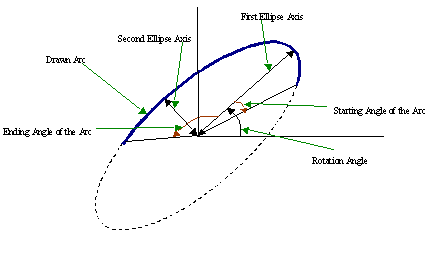
\includegraphics[width=0.5\textwidth]{pics/ellipse.png}

\cvfunc{EllipseBox}

Draws simple or thick elliptic arc or fills ellipse sector.

\cvexp{

void cvEllipseBox( \par CvArr* img, \par CvBox2D box, \par CvScalar color,
                   \par int thickness=1, \par int line\_type=8, \par int shift=0 );

}{CPP}{EllipseBox(img,box,color,thickness=1,line\_type=8,shift=0)-> None}

\begin{description}
\cvarg{img}{Image}
\cvarg{box}{The enclosing box of the ellipse drawn}
\cvarg{thickness}{Thickness of the ellipse boundary}
\cvarg{line\_type}{Type of the ellipse boundary, see \cross{Line} description}
\cvarg{shift}{Number of fractional bits in the box vertex coordinates}
\end{description}

The function \texttt{cvEllipseBox} draws a simple or thick ellipse outline, or fills an ellipse. The functions provides a convenient way to draw an ellipse approximating some shape; that is what \cross{CamShift} and \cross{FitEllipse} do. The ellipse drawn is clipped by ROI rectangle. A piecewise-linear approximation is used for antialiased arcs and thick arcs.

\cvfunc{FillPoly}\label{FillPoly}

Fills polygons interior

\cvexp{

void cvFillPoly( \par CvArr* img,\par CvPoint** pts,\par int* npts,\par int contours,\par CvScalar color,\par int line\_type=8,\par int shift=0 );

}{CPP}{FillPoly(img,pts,color,line\_type=8,shift=0)-> None}

\begin{description}
\cvarg{img}{Image}
\cvarg{pts}{Array of pointers to polygons}
\cvarg{npts}{Array of polygon vertex counters}
\cvarg{contours}{Number of contours that bind the filled region}
\cvarg{color}{Polygon color}
\cvarg{line\_type}{Type of the polygon boundaries, see \cross{Line} description}
\cvarg{shift}{Number of fractional bits in the vertex coordinates}
\end{description}


The function \texttt{cvFillPoly} fills an area bounded by several
polygonal contours. The function fills complex areas, for example,
areas with holes, contour self-intersection, etc.

\cvfunc{FillConvexPoly}\label{FillConvexPoly}

Fills convex polygon

\cvexp{

void cvFillConvexPoly( \par CvArr* img,\par CvPoint* pts,\par int npts,\par CvScalar color,\par int line\_type=8,\par int shift=0 );

}{CPP}{FillConvexPoly(img,pn,color,line\_type=8,shift=0)-> None}

\begin{description}
\cvarg{img}{Image}
\cvarg{pts}{Array of pointers to a single polygon}
\cvarg{npts}{Polygon vertex counter}
\cvarg{color}{Polygon color}
\cvarg{line\_type}{Type of the polygon boundaries, see \cross{Line} description}
\cvarg{shift}{Number of fractional bits in the vertex coordinates}
\end{description}

The function \texttt{cvFillConvexPoly} fills convex polygon interior.
This function is much faster than The function \texttt{cvFillPoly}
and can fill not only the convex polygons but any monotonic polygon,
i.e. a polygon whose contour intersects every horizontal line (scan
line) twice at the most.


\cvfunc{PolyLine}\label{PolyLine}

Draws simple or thick polygons

\cvexp{

void cvPolyLine( \par CvArr* img,\par CvPoint** pts,\par int* npts,\par int contours,\par int is\_closed,\par CvScalar color,\par int thickness=1,\par int line\_type=8,\par int shift=0 );

}{CPP}{PolyLine(img,pts,is\_closed,color,thickness=1,line\_type=8,shift=0)-> None}

\begin{description}
\cvarg{img}{Image}
\cvarg{pts}{Array of pointers to polylines}
\cvarg{npts}{Array of polyline vertex counters}
\cvarg{contours}{Number of polyline contours}
\cvarg{is\_closed}{Indicates whether the polylines must be drawn
closed. If closed, the function draws the line from the last vertex
of every contour to the first vertex.}
\cvarg{color}{Polyline color}
\cvarg{thickness}{Thickness of the polyline edges}
\cvarg{line\_type}{Type of the line segments, see \cross{Line} description}
\cvarg{shift}{Number of fractional bits in the vertex coordinates}
\end{description}

The function \texttt{cvPolyLine} draws a single or multiple polygonal curves.

\subsection{Text}

\cvfunc{InitFont}\label{InitFont}

Initializes font structure

\cvexp{
void cvInitFont( \par CvFont* font,\par int font\_face,\par double hscale,\par double vscale,\par double shear=0,\par int thickness=1,\par int line\_type=8 );
}{CPP}{InitFont(font\_face,hscale,vscale,shear=0,thickness=1,line\_type=8)-> font}

\begin{description}
\cvarg{font}{Pointer to the font structure initialized by the function}
\cvarg{font\_face}{Font name identifier. Only a subset of Hershey fonts \url{http://sources.isc.org/utils/misc/hershey-font.txt} are supported now:
 \begin{description}
 \cvarg{CV\_FONT\_HERSHEY\_SIMPLEX}{normal size sans-serif font}
 \cvarg{CV\_FONT\_HERSHEY\_PLAIN}{small size sans-serif font}
 \cvarg{CV\_FONT\_HERSHEY\_DUPLEX}{normal size sans-serif font (more complex than \texttt{CV\_FONT\_HERSHEY\_SIMPLEX})}
 \cvarg{CV\_FONT\_HERSHEY\_COMPLEX}{normal size serif font}
 \cvarg{CV\_FONT\_HERSHEY\_TRIPLEX}{normal size serif font (more complex than \texttt{CV\_FONT\_HERSHEY\_COMPLEX})}
 \cvarg{CV\_FONT\_HERSHEY\_COMPLEX\_SMALL}{smaller version of \texttt{CV\_FONT\_HERSHEY\_COMPLEX}}
 \cvarg{CV\_FONT\_HERSHEY\_SCRIPT\_SIMPLEX}{hand-writing style font}
 \cvarg{CV\_FONT\_HERSHEY\_SCRIPT\_COMPLEX}{more complex variant of \texttt{CV\_FONT\_HERSHEY\_SCRIPT\_SIMPLEX}}
 \end{description}
 The parameter can be composited from one of the values above and optional \texttt{CV\_FONT\_ITALIC} flag, that means italic or oblique font.}
\cvarg{hscale}{Horizontal scale.  If equal to '1.0f', the characters have the original width depending on the font type. If equal to '0.5f', the characters are of half the original width.}
\cvarg{vscale}{Vertical scale. If equal to '1.0f', the characters have the original height depending on the font type. If equal to '0.5f', the characters are of half the original height.}
\cvarg{shear}{Approximate tangent of the character slope relative to the vertical line.  Zero value means a non-italic font, '1.0f' means ' about 45 degrees ' slope, etc. thickness Thickness of lines composing letters outlines. The function \texttt{cvLine} is used for drawing letters.}
\cvarg{thickness}{Thickness of the text strokes}
\cvarg{line\_type}{Type of the strokes, see \cross{Line} description}
\end{description}

The function \texttt{cvInitFont} initializes the font structure that can be passed to text rendering functions.


\cvfunc{PutText}\label{PutText}

Draws text string

\cvexp{

void cvPutText( \par CvArr* img,\par const char* text,\par CvPoint org,\par const CvFont* font,\par CvScalar color );

}{CPP}{img,text,org,font,color)-> None}

\begin{description}
\cvarg{img}{Input image}
\cvarg{text}{String to print}
\cvarg{org}{Coordinates of the bottom-left corner of the first letter}
\cvarg{font}{Pointer to the font structure}
\cvarg{color}{Text color}
\end{description}


The function \texttt{cvPutText} renders the text in the image with
the specified font and color. The printed text is clipped by ROI
rectangle. Symbols that do not belong to the specified font are
replaced with the rectangle symbol.

\cvfunc{GetTextSize}\label{GetTextSize}

Retrieves width and height of text string

\cvexp{

void cvGetTextSize( \par const char* text\_string,\par const CvFont* font,\par CvSize* text\_size,\par int* baseline );

}{CPP}{GetTextSize(text\_string,font)-> text\_size,baseline}

\begin{description}
\cvarg{font}{Pointer to the font structure}
\cvarg{text\_string}{Input string}
\cvarg{text\_size}{Resultant size of the text string. Height of the text does not include the height of character parts that are below the baseline.}
\cvarg{baseline}{y-coordinate of the baseline relatively to the bottom-most text point}
\end{description}

The function \texttt{cvGetTextSize} calculates the binding rectangle for the given text string when a specified font is used.

\subsection{Point Sets and Contours}

\cvfunc{DrawContours}\label{DrawContours}

Draws contour outlines or interiors in the image

\cvexp{

void cvDrawContours( \par CvArr *img,\par CvSeq* contour,\par CvScalar external\_color,\par CvScalar hole\_color,\par int max\_level,\par int thickness=1,\par int line\_type=8 );

}{CPP}{DrawContours(img,contour,external\_color,hole\_color,max\_level,thickness=1,line\_type=8,offset=(0,0)-> None}

\begin{description}
\cvarg{img}{Image where the contours are to be drawn. Like in any other drawing function, the contours are clipped with the ROI.}
\cvarg{contour}{Pointer to the first contour}
\cvarg{external\_color}{Color of the external contours}
\cvarg{hole\_color}{Color of internal contours (holes)}
\cvarg{max\_level}{Maximal level for drawn contours. If 0, only
\texttt{contour} is drawn. If 1, the contour and all contours after
it on the same level are drawn. If 2, all contours after and all
contours one level below the contours are drawn, etc. If the value
is negative, the function does not draw the contours following after
\texttt{contour} but draws child contours of \texttt{contour} up
to $ |\texttt{max\_level}|-1$ level.}
\cvarg{thickness}{Thickness of lines the contours are drawn with.
If it is negative (e.g. =CV\_FILLED), the contour interiors are
drawn.}
\cvarg{line\_type}{Type of the contour segments, see \cross{Line} description}
\end{description}

The function \texttt{cvDrawContours} draws contour outlines in the image if $\texttt{thickness} \ge 0$ or fills area bounded by the contours if $ \texttt{thickness}<0$.

Example. Connected component detection via contour functions

\begin{lstlisting}

#include "cv.h"
#include "highgui.h"

int main( int argc, char** argv )
{
    IplImage* src;
    // the first command line parameter must be file name of binary (black-n-white) image
    if( argc == 2 && (src=cvLoadImage(argv[1], 0))!= 0)
    {
        IplImage* dst = cvCreateImage( cvGetSize(src), 8, 3 );
        CvMemStorage* storage = cvCreateMemStorage(0);
        CvSeq* contour = 0;

        cvThreshold( src, src, 1, 255, CV_THRESH_BINARY );
        cvNamedWindow( "Source", 1 );
        cvShowImage( "Source", src );

        cvFindContours( src, storage, &contour, sizeof(CvContour), CV_RETR_CCOMP, CV_CHAIN_APPROX_SIMPLE );
        cvZero( dst );

        for( ; contour != 0; contour = contour->h_next )
        {
            CvScalar color = CV_RGB( rand()&255, rand()&255, rand()&255 );
            /* replace CV_FILLED with 1 to see the outlines */
            cvDrawContours( dst, contour, color, color, -1, CV_FILLED, 8 );
        }

        cvNamedWindow( "Components", 1 );
        cvShowImage( "Components", dst );
        cvWaitKey(0);
    }
}

\end{lstlisting}

Replace \texttt{CV\_FILLED} with 1 in the sample below to see the contour outlines

\cvfunc{InitLineIterator}\label{InitLineIterator}

Initializes line iterator

\cvexp{

int cvInitLineIterator( \par const CvArr* image,\par CvPoint pt1,\par CvPoint pt2,\par CvLineIterator* line\_iterator,\par int connectivity=8,\par int left\_to\_right=0 );

}{CPP}{PYTHON}

\begin{description}
\cvarg{image}{Image to sample the line from}
\cvarg{pt1}{First ending point of the line segment}
\cvarg{pt2}{Second ending point of the line segment}
\cvarg{line\_iterator}{Pointer to the line iterator state structure}
\cvarg{connectivity}{The scanned line connectivity, 4 or 8
be always scanned from the left-most point to the right-most out
of \texttt{pt1} and \texttt{pt2} ($ \texttt{left\_to\_right} \ne 0$), or it
is scanned in the specified order, from \texttt{pt1} to \texttt{pt2}
($ \texttt{left\_to\_right} = 0 $ )}
\end{description}

The function \texttt{cvInitLineIterator} initializes the line
iterator and returns the number of pixels between two end points.
Both points must be inside the image. After the iterator has been
initialized, all the points on the raster line that connects the
two ending points may be retrieved by successive calls of
\texttt{CV\_NEXT\_LINE\_POINT} point. The points on the line are
calculated one by one using 4-connected or 8-connected Bresenham
algorithm.

Example. Using line iterator to calculate sum of pixel values along the color line

\begin{lstlisting}

CvScalar sum_line_pixels( IplImage* image, CvPoint pt1, CvPoint pt2 )
{
    CvLineIterator iterator;
    int blue_sum = 0, green_sum = 0, red_sum = 0;
    int count = cvInitLineIterator( image, pt1, pt2, &iterator, 8, 0 );

    for( int i = 0; i < count; i++ ){
        blue_sum += iterator.ptr[0];
        green_sum += iterator.ptr[1];
        red_sum += iterator.ptr[2];
        CV_NEXT_LINE_POINT(iterator);

        /* print the pixel coordinates: demonstrates how to calculate the coordinates */
        {
        int offset, x, y;
        /* assume that ROI is not set, otherwise need to take it into account. */
        offset = iterator.ptr - (uchar*)(image->imageData);
        y = offset/image->widthStep;
        x = (offset - y*image->widthStep)/(3*sizeof(uchar) /* size of pixel */);
        printf("(%d,%d)\n", x, y );
        }
    }
    return cvScalar( blue_sum, green_sum, red_sum );
}

\end{lstlisting}

\cvfunc{ClipLine}\label{ClipLine}

Clips the line against the image rectangle

\cvexp{

int cvClipLine( \par CvSize img\_size,\par CvPoint* pt1,\par CvPoint* pt2 );

}{CPP}{PYTHON}

\begin{description}
\cvarg{img\_size}{Size of the image}
\cvarg{pt1}{First ending point of the line segment. It is modified by the function.}
\cvarg{pt2}{Second ending point of the line segment. It is modified by the function.}
\end{description}

The function \texttt{cvClipLine} calculates a part of the line
segment which is entirely in the image. It returns 0 if the line
segment is completely outside the image and 1 otherwise.

\cvfunc{Ellipse2Poly}\label{Ellipse2Poly}

Approximates elliptic arc with polyline

\cvexp{

int cvEllipse2Poly( \par CvPoint center,\par CvSize axes,\par int angle,\par int arc\_start,\par int arc\_end,\par CvPoint* pts,\par int delta );

}{CPP}{PYTHON}

\begin{description}
\cvarg{center}{Center of the arc}
\cvarg{axes}{Half-sizes of the arc. See \cross{Ellipse}.}
\cvarg{angle}{Rotation angle of the ellipse in degrees. See \cross{Ellipse}}
\cvarg{start\_angle}{Starting angle of the elliptic arc}
\cvarg{end\_angle}{Ending angle of the elliptic arc}
\cvarg{pts}{The array of points, filled by the function}
\cvarg{delta}{Angle between the subsequent polyline vertices, approximation accuracy. So, the total number of output points will
$ \lceil( \texttt{end\_angle} - \texttt{start\_angle} ) / \texttt{delta} \rceil + 1 $
at max.}
\end{description}

The function \texttt{cvEllipse2Poly} computes vertices of the polyline that approximates the specified elliptic arc. It is used by \cross{Ellipse}.

\section{Data Persistence and RTTI}


\subsection{File Storage}

\cvstruct{CvFileStorage}\label{CvFileStorage}

File Storage

\begin{lstlisting}

typedef struct CvFileStorage
{
    ...       // hidden fields
} CvFileStorage;

\end{lstlisting}

The structure \cross{CvFileStorage} is "black box" representation
of file storage that is associated with a file on disk. Several
functions that are described below take \texttt{CvFileStorage} on
input and allow user to save or to load hierarchical collections
that consist of scalar values, standard CXCore objects (such as
matrices, sequences, graphs) and user-defined objects.

CXCore can read and write data in XML (http://www.w3c.org/XML) or YAML
(http://www.yaml.org) formats. Below is the example of $3 \times 3$
floating-point identity matrix \texttt{A}, stored in XML and YAML files
using CXCore functions:

XML:

\begin{verbatim}
<?xml version="1.0">
<opencv_storage>
<A type_id="opencv-matrix">
  <rows>3</rows>
  <cols>3</cols>
  <dt>f</dt>
  <data>1. 0. 0. 0. 1. 0. 0. 0. 1.</data>
</A>
</opencv_storage>
\end{verbatim}

YAML:

\begin{verbatim}
%YAML:1.0
A: !!opencv-matrix
  rows: 3
  cols: 3
  dt: f
  data: [ 1., 0., 0., 0., 1., 0., 0., 0., 1.]
\end{verbatim}

As it can be seen from the examples, XML uses nested tags to represent
hierarchy, while YAML uses indentation for that purpose (similarly
to Python programming language).

The same CXCore functions can read and write data in both formats,
the particular format is determined by the extension of the opened
file, .xml for XML files and .yml or .yaml for YAML.


\cvstruct{CvFileNode}\label{CvFileNode}

File Storage Node

\begin{lstlisting}

/* file node type */
#define CV\_NODE\_NONE        0
#define CV\_NODE\_INT         1
#define CV\_NODE\_INTEGER     CV\_NODE\_INT
#define CV\_NODE\_REAL        2
#define CV\_NODE\_FLOAT       CV\_NODE\_REAL
#define CV\_NODE\_STR         3
#define CV\_NODE\_STRING      CV\_NODE\_STR
#define CV\_NODE\_REF         4 /* not used */
#define CV\_NODE\_SEQ         5
#define CV\_NODE\_MAP         6
#define CV\_NODE\_TYPE\_MASK   7

/* optional flags */
#define CV\_NODE\_USER        16
#define CV\_NODE\_EMPTY       32
#define CV\_NODE\_NAMED       64

#define CV\_NODE\_TYPE(tag)  ((tag) & CV\_NODE\_TYPE\_MASK)

#define CV\_NODE\_IS\_INT(tag)        (CV\_NODE\_TYPE(tag) == CV\_NODE\_INT)
#define CV\_NODE\_IS\_REAL(tag)       (CV\_NODE\_TYPE(tag) == CV\_NODE\_REAL)
#define CV\_NODE\_IS\_STRING(tag)     (CV\_NODE\_TYPE(tag) == CV\_NODE\_STRING)
#define CV\_NODE\_IS\_SEQ(tag)        (CV\_NODE\_TYPE(tag) == CV\_NODE\_SEQ)
#define CV\_NODE\_IS\_MAP(tag)        (CV\_NODE\_TYPE(tag) == CV\_NODE\_MAP)
#define CV\_NODE\_IS\_COLLECTION(tag) (CV\_NODE\_TYPE(tag) >= CV\_NODE\_SEQ)
#define CV\_NODE\_IS\_FLOW(tag)       (((tag) & CV\_NODE\_FLOW) != 0)
#define CV\_NODE\_IS\_EMPTY(tag)      (((tag) & CV\_NODE\_EMPTY) != 0)
#define CV\_NODE\_IS\_USER(tag)       (((tag) & CV\_NODE\_USER) != 0)
#define CV\_NODE\_HAS\_NAME(tag)      (((tag) & CV\_NODE\_NAMED) != 0)

#define CV\_NODE\_SEQ\_SIMPLE 256
#define CV\_NODE\_SEQ\_IS\_SIMPLE(seq) (((seq)->flags & CV\_NODE\_SEQ\_SIMPLE) != 0)

typedef struct CvString
{
    int len;
    char* ptr;
}
CvString;

/* all the keys (names) of elements in the readed file storage
   are stored in the hash to speed up the lookup operations */
typedef struct CvStringHashNode
{
    unsigned hashval;
    CvString str;
    struct CvStringHashNode* next;
}
CvStringHashNode;

/* basic element of the file storage - scalar or collection */
typedef struct CvFileNode
{
    int tag;
    struct CvTypeInfo* info; /* type information
            (only for user-defined object, for others it is 0) */
    union
    {
        double f; /* scalar floating-point number */
        int i;    /* scalar integer number */
        CvString str; /* text string */
        CvSeq* seq; /* sequence (ordered collection of file nodes) */
        struct CvMap* map; /* map (collection of named file nodes) */
    } data;
}
CvFileNode;

\end{lstlisting}

The structure is used only for retrieving data from file storage
(i.e. for loading data from file). When data is written to file,
it is done sequentially, with minimal buffering. No data is stored
in the file storage.

In opposite, when data is read from file, the whole file is parsed
and represented in memory as a tree. Every node of the tree is
represented by \cross{CvFileNode}. Type of the file node \texttt{N}
can be retrieved as \texttt{CV\_NODE\_TYPE(N->tag)}. Some file nodes
(leaves) are scalars: text strings, integer or floating-point
numbers. Other file nodes are collections of file nodes, which can
be scalars or collections in their turn. There are two types of
collections: sequences and maps (we use YAML notation, however, the
same is true for XML streams). Sequences (do not mix them with
\cross{CvSeq}) are ordered collections of unnamed file nodes, maps
are unordered collections of named file nodes. Thus, elements of
sequences are accessed by index (\cross{GetSeqElem}), while elements
of maps are accessed by name (\cross{GetFileNodeByName}). The table
below describes the different types of a file node:

\begin{tabular}{| c | c | c |}
\hline
Type           & \texttt{CV\_NODE\_TYPE(node->tag)} & Value\\ \hline \hline
Integer        & \texttt{CV\_NODE\_INT}             & \texttt{node->data.i} \\ \hline
Floating-point & \texttt{CV\_NODE\_REAL}            & \texttt{node->data.f} \\ \hline
Text string    & \texttt{CV\_NODE\_STR}             & \texttt{node->data.str.ptr} \\ \hline
Sequence       & \texttt{CV\_NODE\_SEQ}             & \texttt{node->data.seq} \\ \hline
Map            & \texttt{CV\_NODE\_MAP}             & \texttt{node->data.map} (see below)\\ \hline
\end{tabular}

There is no need to access \texttt{map} field directly (BTW,
\texttt{CvMap} is a hidden structure). The elements of the map can
be retrieved with \cross{GetFileNodeByName} function that takes
pointer to the "map" file node.

A user (custom) object is instance of either one of standard CxCore
types, such as \cross{CvMat}, \cross{CvSeq} etc., or any type
registered with \cross{RegisterTypeInfo}. Such an object is initially
represented in file as a map (as shown in XML and YAML sample files
above), after file storage has been opened and parsed. Then the
object can be decoded (coverted to the native representation) by
request - when user calls \cross{Read} or \cross{ReadByName} function.


\cvstruct{CvAttrList}\label{CvAttrList}

List of attributes

\begin{lstlisting}

typedef struct CvAttrList
{
    const char** attr; /* NULL-terminated array of (attribute\_name,attribute\_value) pairs */
    struct CvAttrList* next; /* pointer to next chunk of the attributes list */
}
CvAttrList;

/* initializes CvAttrList structure */
inline CvAttrList cvAttrList( const char** attr=NULL, CvAttrList* next=NULL );

/* returns attribute value or 0 (NULL) if there is no such attribute */
const char* cvAttrValue( const CvAttrList* attr, const char* attr\_name );

\end{lstlisting}

In the current implementation attributes are used to pass extra parameters when writing user objects (see \cross{Write}). XML attributes inside tags are not supported, besides the object type specification (\texttt{type\_id} attribute).

\cvfunc{OpenFileStorage}\label{OpenFileStorage}

Opens file storage for reading or writing data

\cvexp{

CvFileStorage* cvOpenFileStorage( \par const char* filename,\par CvMemStorage* memstorage,\par int flags );

}{CPP}{PYTHON}

\begin{description}
\cvarg{filename}{Name of the file associated with the storage}
\cvarg{memstorage}{Memory storage used for temporary data and for
storing dynamic structures, such as \cross{CvSeq} or \cross{CvGraph}.
If it is NULL, a temporary memory storage is created and used.}
\cvarg{flags}{Can be one of the following:
  \begin{description}
  \cvarg{CV\_STORAGE\_READ}{the storage is open for reading}
  \cvarg{CV\_STORAGE\_WRITE}{the storage is open for writing}
  \end{description}}
\end{description}

The function \texttt{cvOpenFileStorage} opens file storage for
reading or writing data. In the latter case a new file is created
or existing file is rewritten. Type of the read of written file is
determined by the filename extension: '.xml' for \texttt{XML}
and '.yml' or '.yaml' for \texttt{YAML}. The function
returns pointer to \cross{CvFileStorage} structure.

\cvfunc{ReleaseFileStorage}\label{ReleaseFileStorage}

Releases file storage

\cvexp{

void  cvReleaseFileStorage( CvFileStorage** fs );

}{CPP}{PYTHON}

\begin{description}
\cvarg{fs}{Double pointer to the released file storage}
\end{description}


The function \texttt{cvReleaseFileStorage} closes the file associated with the storage and releases all the temporary structures. It must be called after all I/O operations with the storage are finished.


\subsection{Writing Data}

\cvfunc{StartWriteStruct}\label{StartWriteStruct}

Starts writing a new structure

\cvexp{

void  cvStartWriteStruct( CvFileStorage* fs,\par const char* name,\par int struct\_flags,\par const char* type\_name=NULL,\par CvAttrList attributes=cvAttrList( \par));

}{CPP}{PYTHON}

\begin{description}
\cvarg{fs}{File storage}
\cvarg{name}{Name of the written structure. The structure can be accessed by this name when the storage is read.}
\cvarg{struct\_flags}{A combination one of the following values:
\begin{description}
\cvarg{CV\_NODE\_SEQ}{the written structure is a sequence (see discussion of \cross{CvFileStorage}), that is, its elements do not have a name.}
\cvarg{CV\_NODE\_MAP}{the written structure is a map (see discussion of \cross{CvFileStorage}), that is, all its elements have names. One and only one of the two above flags must be specified}
\end{description}}
\cvarg{CV\_NODE\_FLOW}{the optional flag that has sense only for YAML streams. It means that the structure is written as a flow (not as a block), which is more compact. It is recommended to use this flag for structures or arrays whose elements are all scalars.}
\cvarg{type\_name}{Optional parameter - the object type name. In
case of XML it is written as \texttt{type\_id} attribute of the
structure opening tag. In case of YAML it is written after a colon
following the structure name (see the example in \cross{CvFileStorage}
description). Mainly it comes with user objects. When the storage
is read, the encoded type name is used to determine the object type
(see \cross{CvTypeInfo} and \cross{FindTypeInfo}).}
\cvarg{attributes}{This parameter is not used in the current implementation}
\end{description}

The function \texttt{cvStartWriteStruct} starts writing a compound
structure (collection) that can be a sequence or a map. After all
the structure fields, which can be scalars or structures, are
written, \cross{EndWriteStruct} should be called. The function can
be used to group some objects or to implement \texttt{write}
function for a some user object (see \cross{CvTypeInfo}).

\cvfunc{EndWriteStruct}\label{EndWriteStruct}

Ends writing a structure

\cvexp{

void  cvEndWriteStruct( CvFileStorage* fs );

}{CPP}{PYTHON}

\begin{description}
\cvarg{fs}{File storage}
\end{description}


The function \texttt{cvEndWriteStruct} finishes the currently written structure.

\cvfunc{WriteInt}\label{WriteInt}

Writes an integer value

\cvexp{

void  cvWriteInt( \par CvFileStorage* fs,\par const char* name,\par int value );

}{CPP}{PYTHON}

\begin{description}
\cvarg{fs}{File storage}
\cvarg{name}{Name of the written value. Should be NULL if and only if the parent structure is a sequence.}
\cvarg{value}{The written value}
\end{description}

The function \texttt{cvWriteInt} writes a single integer value (with or without a name) to the file storage.

\cvfunc{WriteReal}\label{WriteReal}

Writes a floating-point value

\cvexp{

void  cvWriteReal( \par CvFileStorage* fs,\par const char* name,\par double value );

}{CPP}{PYTHON}

\begin{description}
\cvarg{fs}{File storage}
\cvarg{name}{Name of the written value. Should be NULL if and only if the parent structure is a sequence.}
\cvarg{value}{The written value}
\end{description}

The function \texttt{cvWriteReal} writes a single floating-point
value (with or without a name) to the file storage. The special
values are encoded: NaN (Not A Number) as .NaN, $ \pm \infty $ as +.Inf
(-.Inf).

The following example shows how to use the low-level writing functions
to store custom structures, such as termination criteria, without
registering a new type.

\begin{lstlisting}

void write_termcriteria( CvFileStorage* fs, const char* struct_name,
                         CvTermCriteria* termcrit )
{
    cvStartWriteStruct( fs, struct_name, CV_NODE_MAP, NULL, cvAttrList(0,0));
    cvWriteComment( fs, "termination criteria", 1 ); // just a description
    if( termcrit->type & CV_TERMCRIT_ITER )
        cvWriteInteger( fs, "max_iterations", termcrit->max_iter );
    if( termcrit->type & CV_TERMCRIT_EPS )
        cvWriteReal( fs, "accuracy", termcrit->epsilon );
    cvEndWriteStruct( fs );
}

\end{lstlisting}

\cvfunc{WriteString}\label{WriteString}

Writes a text string

\cvexp{

void  cvWriteString( \par CvFileStorage* fs,\par const char* name,\par const char* str,\par int quote=0 );

}{CPP}{PYTHON}

\begin{description}
\cvarg{fs}{File storage}
\cvarg{name}{Name of the written string . Should be NULL if and only if the parent structure is a sequence.}
\cvarg{str}{The written text string}
\cvarg{quote}{If non-zero, the written string is put in quotes, regardless of whether they are required or not. Otherwise, if the flag is zero, quotes are used only when they are required (e.g. when the string starts with a digit or contains spaces).}
\end{description}

The function \texttt{cvWriteString} writes a text string to the file storage.

\cvfunc{WriteComment}\label{WriteComment}

Writes comment

\cvexp{

void  cvWriteComment( \par CvFileStorage* fs,\par const char* comment,\par int eol\_comment );

}{CPP}{PYTHON}

\begin{description}
\cvarg{fs}{File storage}
\cvarg{comment}{The written comment, single-line or multi-line}
\cvarg{eol\_comment}{If non-zero, the function tries to put the comment in the end of current line. If the flag is zero, if the comment is multi-line, or if it does not fit in the end of the current line, the comment starts from a new line.}
\end{description}

The function \texttt{cvWriteComment} writes a comment into the file storage. The comments are skipped when the storage is read, so they may be used only for debugging or descriptive purposes.

\cvfunc{StartNextStream}\label{StartNextStream}

Starts the next stream

\cvexp{

void  cvStartNextStream( CvFileStorage* fs );

}{CPP}{PYTHON}

\begin{description}
\cvarg{fs}{File storage}
\end{description}


The function \texttt{cvStartNextStream} starts the next stream in the file storage. Both YAML and XML supports multiple "streams". This is useful for concatenating files or for resuming the writing process.


\cvfunc{Write}\label{Write}

Writes user object

\cvexp{

void  cvWrite( CvFileStorage* fs,\par const char* name,\par const void* ptr,\par CvAttrList attributes=cvAttrList( \par) );

}{CPP}{PYTHON}

\begin{description}
\cvarg{fs}{File storage}
\cvarg{name}{Name, of the written object. Should be NULL if and only if the parent structure is a sequence.}
\cvarg{ptr}{Pointer to the object}
\cvarg{attributes}{The attributes of the object. They are specific for each particular type (see the dicsussion).}
\end{description}

The function \texttt{cvWrite} writes the object to file storage. First, the appropriate type info is found using \cross{TypeOf}. Then, \texttt{write} method of the type info is called.

Attributes are used to customize the writing procedure. The standard types support the following attributes (all the \texttt{*dt} attributes have the same format as in \cross{WriteRawData}):

CvSeq
  \begin{description}
  \cvarg{header\_dt}{description of user fields of the sequence header that follow CvSeq, or CvChain (if the sequence is Freeman chain) or CvContour (if the sequence is a contour or point sequence)}
  \cvarg{dt}{description of the sequence elements.}
  \cvarg{recursive}{if the attribute is present and is not equal to "0" or "false", the whole tree of sequences (contours) is stored.}
  \end{description}
Cvgraph
  \begin{description}
  \cvarg{header\_dt}{description of user fields of the graph header that follow CvGraph;}
  \cvarg{vertex\_dt}{description of user fields of graph vertices}
  \cvarg{edge\_dt}{description of user fields of graph edges (note, that edge weight is always written, so there is no need to specify it explicitly)}
  \end{description}

Below is the code that creates the YAML file shown in \texttt{CvFileStorage} description:

\begin{lstlisting}

#include "cxcore.h"

int main( int argc, char** argv )
{
    CvMat* mat = cvCreateMat( 3, 3, CV\_32F );
    CvFileStorage* fs = cvOpenFileStorage( "example.yml", 0, CV\_STORAGE\_WRITE );

    cvSetIdentity( mat );
    cvWrite( fs, "A", mat, cvAttrList(0,0) );

    cvReleaseFileStorage( &fs );
    cvReleaseMat( &mat );
    return 0;
}

\end{lstlisting}


\cvfunc{WriteRawData}\label{WriteRawData}

Writes multiple numbers

\cvexp{

void  cvWriteRawData( \par CvFileStorage* fs,\par const void* src,\par int len,\par const char* dt );

}{CPP}{PYTHON}

\begin{description}
\cvarg{fs}{File storage}
\cvarg{src}{Pointer to the written array}
\cvarg{len}{Number of the array elements to write}
\cvarg{dt}{Specification of each array element that has the following format
\texttt{([count]\{'u'|'c'|'w'|'s'|'i'|'f'|'d'\})...}
where the characters correspond to fundamental C types:
\begin{description}
 \cvarg{u}{8-bit unsigned number}
 \cvarg{c}{8-bit signed number}
 \cvarg{w}{16-bit unsigned number}
 \cvarg{s}{16-bit signed number}
 \cvarg{i}{32-bit signed number}
 \cvarg{f}{single precision floating-point number}
 \cvarg{d}{double precision floating-point number}
 \cvarg{r}{pointer. 32 lower bits of it are written as a signed integer. The type can be used to store structures with links between the elements.
\texttt{count} is the optional counter of values of the certain type. For
example, \texttt{2if} means that each array element is a structure
of 2 integers, followed by a single-precision floating-point number. The
equivalent notations of the above specification are '\texttt{iif}',
'\texttt{2i1f}' etc. Other examples: \texttt{u} means that the
array consists of bytes, \texttt{2d} - the array consists of pairs
of doubles.}
\end{description}}
\end{description}

The function \texttt{cvWriteRawData} writes array, which elements consist
of a single of multiple numbers. The function call can be replaced with
a loop containing a few \cross{WriteInt} and \cross{WriteReal} calls, but
a single call is more efficient. Note, that because none of the elements
have a name, they should be written to a sequence rather than a map.

\cvfunc{WriteFileNode}\label{WriteFileNode}

Writes file node to another file storage

\cvexp{

void cvWriteFileNode( \par CvFileStorage* fs,\par const char* new\_node\_name,\par const CvFileNode* node,\par int embed );

}{CPP}{PYTHON}

\begin{description}
\cvarg{fs}{Destination file storage}
\cvarg{new\_file\_node}{New name of the file node in the destination file storage. To keep the existing name, use \cross{cvGetFileNodeName}}
\cvarg{node}{The written node}
\cvarg{embed}{If the written node is a collection and this parameter is not zero, no extra level of hiararchy is created. Instead, all the elements of \texttt{node} are written into the currently written structure. Of course, map elements may be written only to map, and sequence elements may be written only to sequence.}
\end{description}

The function \texttt{cvWriteFileNode} writes a copy of file node to file storage. The possible application of the function are: merging several file storages into one. Conversion between XML and YAML formats etc.

\subsection{Reading Data}

Data are retrieved from file storage in 2 steps: first, the file node
containing the requested data is found; then, data is extracted from
the node manually or using custom \texttt{read} method.

\cvfunc{GetRootFileNode}\label{GetRootFileNode}

Retrieves one of top-level nodes of the file storage

\cvexp{

CvFileNode* cvGetRootFileNode( \par const CvFileStorage* fs,\par int stream\_index=0 );

}{CPP}{PYTHON}

\begin{description}
\cvarg{fs}{File storage}
\cvarg{stream\_index}{Zero-based index of the stream. See \cross{StartNextStream}. In most cases, there is only one stream in the file, however there can be several.}
\end{description}

The function \texttt{cvGetRootFileNode} returns one of top-level file
nodes. The top-level nodes do not have a name, they correspond to the
streams, that are stored one after another in the file storage. If the
index is out of range, the function returns NULL pointer, so all the
top-level nodes may be iterated by subsequent calls to the function with
'stream\_index=0,1,...', until NULL pointer is returned. This function
may be used as a base for recursive traversal of the file storage.

\cvfunc{GetFileNodeByName}\label{GetFileNodeByName}

Finds node in the map or file storage

\cvexp{

CvFileNode* cvGetFileNodeByName( \par const CvFileStorage* fs,\par const CvFileNode* map,\par const char* name );

}{CPP}{PYTHON}

\begin{description}
\cvarg{fs}{File storage}
\cvarg{map}{The parent map. If it is NULL, the function searches in all the top-level nodes (streams), starting from the first one.}
\cvarg{name}{The file node name}
\end{description}


The function \texttt{cvGetFileNodeByName} finds a file node by
\texttt{name}. The node is searched either in \texttt{map} or, if the
pointer is NULL, among the top-level file nodes of the storage. Using
this function for maps and \cross{GetSeqElem} (or sequence reader)
for sequences, it is possible to nagivate through the file storage. To
speed up multiple queries for a certain key (e.g. in case of array
of structures) one may use a pair of \cross{GetHashedKey} and
\cross{GetFileNode}.

\cvfunc{GetHashedKey}\label{GetHashedKey}

Returns a unique pointer for given name

\cvexp{

CvStringHashNode* cvGetHashedKey( \par CvFileStorage* fs,\par const char* name,\par int len=-1,\par int create\_missing=0 );

}{CPP}{PYTHON}

\begin{description}
\cvarg{fs}{File storage}
\cvarg{name}{Literal node name}
\cvarg{len}{Length of the name (if it is known apriori), or -1 if it needs to be calculated}
\cvarg{create\_missing}{Flag that specifies, whether an absent key should be added into the hash table, or not}
\end{description}

The function \texttt{cvGetHashedKey} returns the unique pointer for
each particular file node name. This pointer can be then passed to
\cross{GetFileNode} function that is faster than \cross{GetFileNodeByName}
because it compares text strings by comparing pointers rather than the
strings' content.

Consider the following example: an array of points is encoded as a sequence of 2-entry maps, e.g.:

\begin{lstlisting}

%YAML:1.0
points:
  - { x: 10, y: 10 }
  - { x: 20, y: 20 }
  - { x: 30, y: 30 }
  # ...

\end{lstlisting}

Then, it is possible to get hashed "x" and "y" pointers to speed up decoding of the points.

Example. Reading an array of structures from file storage

\begin{lstlisting}

#include "cxcore.h"

int main( int argc, char** argv )
{
    CvFileStorage* fs = cvOpenFileStorage( "points.yml", 0, CV\_STORAGE\_READ );
    CvStringHashNode* x\_key = cvGetHashedNode( fs, "x", -1, 1 );
    CvStringHashNode* y\_key = cvGetHashedNode( fs, "y", -1, 1 );
    CvFileNode* points = cvGetFileNodeByName( fs, 0, "points" );

    if( CV\_NODE\_IS\_SEQ(points->tag) )
    {
        CvSeq* seq = points->data.seq;
        int i, total = seq->total;
        CvSeqReader reader;
        cvStartReadSeq( seq, &reader, 0 );
        for( i = 0; i < total; i++ )
        {
            CvFileNode* pt = (CvFileNode*)reader.ptr;
#if 1 /* faster variant */
            CvFileNode* xnode = cvGetFileNode( fs, pt, x\_key, 0 );
            CvFileNode* ynode = cvGetFileNode( fs, pt, y\_key, 0 );
            assert( xnode && CV\_NODE\_IS\_INT(xnode->tag) &&
                    ynode && CV\_NODE\_IS\_INT(ynode->tag));
            int x = xnode->data.i; // or x = cvReadInt( xnode, 0 );
            int y = ynode->data.i; // or y = cvReadInt( ynode, 0 );
#elif 1 /* slower variant; does not use x\_key & y\_key */
            CvFileNode* xnode = cvGetFileNodeByName( fs, pt, "x" );
            CvFileNode* ynode = cvGetFileNodeByName( fs, pt, "y" );
            assert( xnode && CV\_NODE\_IS\_INT(xnode->tag) &&
                    ynode && CV\_NODE\_IS\_INT(ynode->tag));
            int x = xnode->data.i; // or x = cvReadInt( xnode, 0 );
            int y = ynode->data.i; // or y = cvReadInt( ynode, 0 );
#else /* the slowest yet the easiest to use variant */
            int x = cvReadIntByName( fs, pt, "x", 0 /* default value */ );
            int y = cvReadIntByName( fs, pt, "y", 0 /* default value */ );
#endif
            CV\_NEXT\_SEQ\_ELEM( seq->elem\_size, reader );
            printf("%d: (%d, %d)\n", i, x, y );
        }
    }
    cvReleaseFileStorage( &fs );
    return 0;
}

\end{lstlisting}

Please note that, whatever method of accessing map you are using, it is
still much slower than using plain sequences, for example, in the above
sample, it is more efficient to encode the points as pairs of integers
in the single numeric sequence.

\cvfunc{GetFileNode}\label{GetFileNode}

Finds node in the map or file storage

\cvexp{

CvFileNode* cvGetFileNode( \par CvFileStorage* fs,\par CvFileNode* map,\par const CvStringHashNode* key,\par int create\_missing=0 );

}{CPP}{PYTHON}

\begin{description}
\cvarg{fs}{File storage}
\cvarg{map}{The parent map. If it is NULL, the function searches a top-level node. If both \texttt{map} and \texttt{key} are NULLs, the function returns the root file node - a map that contains top-level nodes.}
\cvarg{key}{Unique pointer to the node name, retrieved with \cross{GetHashedKey}}
\cvarg{create\_missing}{Flag that specifies, whether an absent node should be added to the map, or not}
\end{description}


The function \texttt{cvGetFileNode} finds a file node. It is a faster version \cross{GetFileNodeByName} (see \cross{GetHashedKey} discussion). Also, the function can insert a new node, if it is not in the map yet (which is used by parsing functions).

\cvfunc{GetFileNodeName}\label{GetFileNodeName}

Returns name of file node

\cvexp{

const char* cvGetFileNodeName( const CvFileNode* node );

}{CPP}{PYTHON}

\begin{description}
\cvarg{node}{File node}
\end{description}


The function \texttt{cvGetFileNodeName} returns name of the file node or NULL, if the file node does not have a name, or if \texttt{node} is \texttt{NULL}.


\cvfunc{ReadInt}\label{ReadInt}

Retrieves integer value from file node

\cvexp{

int cvReadInt( \par const CvFileNode* node,\par int default\_value=0 );

}{CPP}{PYTHON}

\begin{description}
\cvarg{node}{File node}
\cvarg{default\_value}{The value that is returned if \texttt{node} is NULL}
\end{description}


The function \texttt{cvReadInt} returns integer that is represented
by the file node. If the file node is NULL, \texttt{default\_value}
is returned (thus, it is convenient to call the function right after
\cross{GetFileNode} without checking for NULL pointer), otherwise if
the file node has type \texttt{CV\_NODE\_INT}, then \texttt{node->data.i} is
returned, otherwise if the file node has type \texttt{CV\_NODE\_REAL},
then \texttt{node->data.f} is converted to integer and returned, otherwise the
result is not determined.

\cvfunc{ReadIntByName}\label{ReadIntByName}

Finds file node and returns its value

\cvexp{

int cvReadIntByName( \par const CvFileStorage* fs,\par const CvFileNode* map,\par const char* name,\par int default\_value=0 );

}{CPP}{PYTHON}

\begin{description}
\cvarg{fs}{File storage}
\cvarg{map}{The parent map. If it is NULL, the function searches a top-level node.}
\cvarg{name}{The node name}
\cvarg{default\_value}{The value that is returned if the file node is not found}
\end{description}

The function \texttt{cvReadIntByName} is a simple superposition of \cross{GetFileNodeByName} and \cross{ReadInt}.


\cvfunc{ReadReal}\label{ReadReal}

Retrieves floating-point value from file node

\cvexp{

double cvReadReal( \par const CvFileNode* node,\par double default\_value=0. );

}{CPP}{PYTHON}

\begin{description}
\cvarg{node}{File node}
\cvarg{default\_value}{The value that is returned if \texttt{node} is NULL}
\end{description}

The function \texttt{cvReadReal} returns floating-point value
that is represented by the file node. If the file node is NULL,
\texttt{default\_value} is returned (thus, it is convenient to call
the function right after \cross{GetFileNode} without checking for NULL
pointer), otherwise if the file node has type \texttt{CV\_NODE\_REAL},
then \texttt{node->data.f} is returned, otherwise if the file node has type
\texttt{CV\_NODE\_INT}, then 'node->data.f' is converted to floating-point
and returned, otherwise the result is not determined.

\cvfunc{ReadRealByName}\label{ReadRealByName}

Finds file node and returns its value

\cvexp{

double  cvReadRealByName( \par const CvFileStorage* fs,\par const CvFileNode* map,\par const char* name,\par double default\_value=0. );

}{CPP}{PYTHON}

\begin{description}
\cvarg{fs}{File storage}
\cvarg{map}{The parent map. If it is NULL, the function searches a top-level node.}
\cvarg{name}{The node name}
\cvarg{default\_value}{The value that is returned if the file node is not found}
\end{description}

The function \texttt{cvReadRealByName} is a simple superposition of \cross{GetFileNodeByName} and \cross{ReadReal}.

\cvfunc{ReadString}\label{ReadString}

Retrieves text string from file node

\cvexp{

const char* cvReadString( \par const CvFileNode* node,\par const char* default\_value=NULL );

}{CPP}{PYTHON}

\begin{description}
\cvarg{node}{File node}
\cvarg{default\_value}{The value that is returned if \texttt{node} is NULL}
\end{description}

The function \texttt{cvReadString} returns text string that is represented
by the file node. If the file node is NULL, \texttt{default\_value}
is returned (thus, it is convenient to call the function right after
\cross{GetFileNode} without checking for NULL pointer), otherwise if
the file node has type \texttt{CV\_NODE\_STR}, then 'node->data.str.ptr'
is returned, otherwise the result is not determined.

\cvfunc{ReadStringByName}\label{ReadStringByName}

Finds file node and returns its value

\cvexp{

const char* cvReadStringByName( \par const CvFileStorage* fs,\par const CvFileNode* map,\par const char* name,\par const char* default\_value=NULL );

}{CPP}{PYTHON}

\begin{description}
\cvarg{fs}{File storage}
\cvarg{map}{The parent map. If it is NULL, the function searches a top-level node.}
\cvarg{name}{The node name}
\cvarg{default\_value}{The value that is returned if the file node is not found}
\end{description}

The function \texttt{cvReadStringByName} is a simple superposition of \cross{GetFileNodeByName} and \cross{ReadString}.

\cvfunc{Read}\label{Read}

Decodes object and returns pointer to it

\cvexp{

void* cvRead( \par CvFileStorage* fs,\par CvFileNode* node,\par CvAttrList* attributes=NULL );

}{CPP}{PYTHON}

\begin{description}
\cvarg{fs}{File storage}
\cvarg{node}{The root object node}
\cvarg{attributes}{Unused parameter}
\end{description}

The function \texttt{cvRead} decodes user object (creates object in a
native representation from the file storage subtree) and returns it. The
object to be decoded must be an instance of registered type that supports
\texttt{read} method (see \cross{CvTypeInfo}). Type of the object is
determined by the type name that is encoded in the file. If the object
is dynamic structure, it is created either in memory storage, passed to
\cross{OpenFileStorage} or, if NULL pointer was passed, in temporary
memory storage, which is release when \cross{ReleaseFileStorage} is
called. Otherwise, if the object is not a dynamic structure, it is
created in heap and should be released with a specialized function or
using generic \cross{Release}.

\cvfunc{ReadByName}\label{ReadByName}

Finds object and decodes it

\cvexp{

void* cvReadByName( \par CvFileStorage* fs,\par const CvFileNode* map,\par const char* name,\par CvAttrList* attributes=NULL );

}{CPP}{PYTHON}

\begin{description}
\cvarg{fs}{File storage}
\cvarg{map}{The parent map. If it is NULL, the function searches a top-level node.}
\cvarg{name}{The node name}
\cvarg{attributes}{Unused parameter}
\end{description}

The function \texttt{cvReadByName} is a simple superposition of \cross{GetFileNodeByName} and \cross{Read}.

\cvfunc{ReadRawData}\label{ReadRawData}

Reads multiple numbers

\cvexp{

void cvReadRawData( \par const CvFileStorage* fs,\par const CvFileNode* src,\par void* dst,\par const char* dt );

}{CPP}{PYTHON}

\begin{description}
\cvarg{fs}{File storage}
\cvarg{src}{The file node (a sequence) to read numbers from}
\cvarg{dst}{Pointer to the destination array}
\cvarg{dt}{Specification of each array element. It has the same format as in \cross{WriteRawData}.}
\end{description}

The function \texttt{cvReadRawData} reads elements from a file node that represents a sequence of scalars

\cvfunc{StartReadRawData}\label{StartReadRawData}

Initializes file node sequence reader

\cvexp{

void cvStartReadRawData( \par const CvFileStorage* fs,\par const CvFileNode* src,\par CvSeqReader* reader );

}{CPP}{PYTHON}

\begin{description}
\cvarg{fs}{File storage}
\cvarg{src}{The file node (a sequence) to read numbers from}
\cvarg{reader}{Pointer to the sequence reader}
\end{description}

The function \texttt{cvStartReadRawData} initializes sequence reader to read data from file node. The initialized reader can be then passed to \cross{ReadRawDataSlice}.

\cvfunc{ReadRawDataSlice}\label{ReadRawDataSlice}

Initializes file node sequence reader

\cvexp{

void cvReadRawDataSlice( \par const CvFileStorage* fs,\par CvSeqReader* reader,\par int count,\par void* dst,\par const char* dt );

}{CPP}{PYTHON}

\begin{description}
\cvarg{fs}{File storage}
\cvarg{reader}{The sequence reader. Initialize it with \cross{StartReadRawData}.}
\cvarg{count}{The number of elements to read}
\cvarg{dst}{Pointer to the destination array}
\cvarg{dt}{Specification of each array element. It has the same format as in \cross{WriteRawData}.}
\end{description}

The function \texttt{cvReadRawDataSlice} reads one or more elements from
the file node, representing a sequence, to user-specified array. The
total number of read sequence elements is a product of \texttt{total}
and the number of components in each array element. For example, if
dt=\texttt{2if}, the function will read total*3 sequence elements. As
with any sequence, some parts of the file node sequence may be skipped or
read repeatedly by repositioning the reader using \cross{SetSeqReaderPos}.

\subsection{RTTI and Generic Functions}

\cvstruct{CvTypeInfo}\label{CvTypeInfo}

Type information

\begin{lstlisting}

typedef int (CV_CDECL *CvIsInstanceFunc)( const void* struct_ptr );
typedef void (CV_CDECL *CvReleaseFunc)( void** struct_dblptr );
typedef void* (CV_CDECL *CvReadFunc)( CvFileStorage* storage, CvFileNode* node );
typedef void (CV_CDECL *CvWriteFunc)( CvFileStorage* storage,
                                      const char* name,
                                      const void* struct_ptr,
                                      CvAttrList attributes );
typedef void* (CV_CDECL *CvCloneFunc)( const void* struct_ptr );

typedef struct CvTypeInfo
{
    int flags; /* not used */
    int header_size; /* sizeof(CvTypeInfo) */
    struct CvTypeInfo* prev; /* previous registered type in the list */
    struct CvTypeInfo* next; /* next registered type in the list */
    const char* type_name; /* type name, written to file storage */

    /* methods */
    CvIsInstanceFunc is_instance; /* checks if the passed object belongs to the type */
    CvReleaseFunc release; /* releases object (memory etc.) */
    CvReadFunc read; /* reads object from file storage */
    CvWriteFunc write; /* writes object to file storage */
    CvCloneFunc clone; /* creates a copy of the object */
}
CvTypeInfo;

\end{lstlisting}

The structure \cross{CvTypeInfo} contains information about one of
standard or user-defined types. Instances of the type may or may not
contain pointer to the corresponding \cross{CvTypeInfo} structure. In
any case there is a way to find type info structure for given object -
using \cross{TypeOf} function. Aternatively, type info can be found by
the type name using \cross{FindType}, which is used when object is read
from file storage. User can register a new type with \cross{RegisterType}
that adds the type information structure into the beginning of the type
list - thus, it is possible to create specialized types from generic
standard types and override the basic methods.

\cvfunc{RegisterType}\label{RegisterType}

Registers new type

\cvexp{

void cvRegisterType( const CvTypeInfo* info );

}{CPP}{PYTHON}

\begin{description}
\cvarg{info}{Type info structure}
\end{description}

The function \texttt{cvRegisterType} registers a new type, which is
described by \texttt{info}. The function creates a copy of the structure,
so user should delete it after calling the function.

\cvfunc{UnregisterType}\label{UnregisterType}

Unregisters the type

\cvexp{

void cvUnregisterType( const char* type\_name );

}{CPP}{PYTHON}

\begin{description}
\cvarg{type\_name}{Name of the unregistered type}
\end{description}

The function \texttt{cvUnregisterType} unregisters the type with
the specified name. If the name is unknown, it is possible to locate
the type info by an instance of the type using \cross{TypeOf} or by
iterating the type list, starting from \cross{FirstType}, and then call
\texttt{cvUnregisterType(info->type\_name)}.

\cvfunc{FirstType}\label{FirstType}

Returns the beginning of type list

\cvexp{

CvTypeInfo* cvFirstType( void );

}{CPP}{PYTHON}

The function \texttt{cvFirstType} returns the first type of the list of registered types. Navigation through the list can be done via \texttt{prev} and \texttt{next} fields of \cross{CvTypeInfo} structure.

\cvfunc{FindType}\label{FindType}

Finds type by its name

\cvexp{

CvTypeInfo* cvFindType( const char* type\_name );

}{CPP}{PYTHON}

\begin{description}
\cvarg{type\_name}{Type name}
\end{description}

The function \texttt{cvFindType} finds a registered type by its name. It returns NULL, if there is no type with the specified name.


\cvfunc{TypeOf}\label{TypeOf}

Returns type of the object

\cvexp{

CvTypeInfo* cvTypeOf( const void* struct\_ptr );

}{CPP}{PYTHON}

\begin{description}
\cvarg{struct\_ptr}{The object pointer}
\end{description}

The function \texttt{cvTypeOf} finds the type of given object. It iterates
through the list of registered types and calls \texttt{is\_instance}
function/method of every type info structure with the object until one
of them return non-zero or until the whole list has been traversed. In
the latter case the function returns NULL.

\cvfunc{Release}\label{Release}

Releases the object

\cvexp{

void cvRelease( void** struct\_ptr );

}{CPP}{PYTHON}

\begin{description}
\cvarg{struct\_ptr}{Double pointer to the object}
\end{description}

The function \texttt{cvRelease} finds the type of given object and calls \texttt{release} with the double pointer.

\cvfunc{Clone}\label{Clone}

Makes a clone of the object

\cvexp{

void* cvClone( const void* struct\_ptr );

}{CPP}{PYTHON}

\begin{description}
\cvarg{struct\_ptr}{The object to clone}
\end{description}

The function \texttt{cvClone} finds the type of given object and calls \texttt{clone} with the passed object.

\cvfunc{Save}\label{Save}

Saves object to file

\cvexp{

void cvSave( \par const char* filename,\par const void* struct\_ptr,\par const char* name=NULL,\par const char* comment=NULL,\par CvAttrList attributes=cvAttrList());

}{CPP}{Save(filename,struct\_ptr,name=NULL,comment=NULL)-> None}

\begin{description}
\cvarg{filename}{File name}
\cvarg{struct\_ptr}{Object to save}
\cvarg{name}{Optional object name. If it is NULL, the name will be formed from \texttt{filename}.}
\cvarg{comment}{Optional comment to put in the beginning of the file}
\cvarg{attributes}{Optional attributes passed to \cross{Write}}
\end{description}

The function \texttt{cvSave} saves object to file. It provides a simple interface to \cross{Write}.

\cvfunc{Load}\label{Load}

Loads object from file

\cvexp{

void* cvLoad( \par const char* filename,\par CvMemStorage* memstorage=NULL,\par const char* name=NULL,\par const char** real\_name=NULL );

}{CPP}{Load(filename,storage=NULL,name=NULL)-> generic}

\begin{description}
\cvarg{filename}{File name}
\cvarg{memstorage}{Memory storage for dynamic structures, such as \cross{CvSeq} or \cross{CvGraph} . It is not used for matrices or images.}
\cvarg{name}{Optional object name. If it is NULL, the first top-level object in the storage will be loaded.}
\cvarg{real\_name}{Optional output parameter that will contain name of the loaded object (useful if \texttt{name=NULL})}
\end{description}

The function \texttt{cvLoad} loads object from file. It provides a
simple interface to \cross{Read}. After object is loaded, the file
storage is closed and all the temporary buffers are deleted. Thus,
to load a dynamic structure, such as sequence, contour or graph, one
should pass a valid destination memory storage to the function.

\section{Miscellaneous Functions}

\subsection{Miscellaneous Functions}

\cvfunc{CheckArr}\label{CheckArr}

Checks every element of input array for invalid values

\cvexp{

int  cvCheckArr( \par const CvArr* arr,\par int flags=0,\par double min\_val=0,\par double max\_val=0);

}{CPP}{CheckArr(arr,flags=0,min\_val=0,max\_val=0)-> int}
\begin{lstlisting}
#define cvCheckArray cvCheckArr
\end{lstlisting}

\begin{description}
\cvarg{arr}{The array to check}
\cvarg{flags}{The operation flags, 0 or combination of:
\begin{description}
\cvarg{CV\_CHECK\_RANGE}{if set, the function checks that every value of array is within [minVal,maxVal) range, otherwise it just checks that every element is neither NaN nor $\pm \infty$.}
\cvarg{CV\_CHECK\_QUIET}{if set, the function does not raises an error if an element is invalid or out of range}
\end{description}}
\cvarg{min\_val}{The inclusive lower boundary of valid values range. It is used only if \texttt{CV\_CHECK\_RANGE} is set.}
\cvarg{max\_val}{The exclusive upper boundary of valid values range. It is used only if \texttt{CV\_CHECK\_RANGE} is set.}
\end{description}

The function \texttt{cvCheckArr} checks that every array element is
neither NaN nor $ \pm \infty $.
If \texttt{CV\_CHECK\_RANGE} is set, it also
checks that every element is greater than or equal to \texttt{minVal}
and less than \texttt{maxVal}. The function returns nonzero if the
check succeeded, i.e. all elements are valid and within the range,
and zero otherwise. In the latter case if \texttt{CV\_CHECK\_QUIET}
flag is not set, the function raises runtime error.

\cvfunc{KMeans2}\label{KMeans2}

Splits set of vectors by given number of clusters

\cvexp{
void cvKMeans2( \par const CvArr* samples,\par int cluster\_count,\par CvArr* labels,\par CvTermCriteria termcrit );
}{CPP}{KMeans2(samples,cluster\_count,labels,termcrit)-> None}

\begin{description}
\cvarg{samples}{Floating-point matrix of input samples, one row per sample}
\cvarg{cluster\_count}{Number of clusters to split the set by}
\cvarg{labels}{Output integer vector storing cluster indices for every sample}
\cvarg{termcrit}{Specifies maximum number of iterations and/or accuracy (distance the centers move by between the subsequent iterations)}
\cvarg{attempts}{How many times the algorithm is executed using different initial labelings. The algorithm returns labels that yield the best compactness (see the last function parameter)}
\cvarg{rng}{Optional external random number generator; can be used to fully control the function behaviour. }
\cvarg{flags}{Can be 0 or \texttt{CV\_KMEANS\_USE\_INITIAL\_LABELS}. The latter
value means that during the first (and possibly the only) attempt the
function uses the user-supplied labels as the initial approximation,
instead of generating random labels. For the second and further attempts
the function will use randomly generated labels in any case.}
\cvarg{centers}{The optional output array of the cluster centers. }
\cvarg{compactness}{The optional output parameter, which is computed as
\[
\sum_i ||\texttt{samples}_i - \texttt{centers}_{\texttt{labels}_i}||^2
\]
after every attempt; the best (minimum) value is chosen and the
corresponding labels are returned by the function. Basically,
user can use only the core of the function, set the number of
attempts to 1, initialize labels each time using a custom algorithm
(\texttt{flags}=\texttt{CV\_KMEAN\_USE\_INITIAL\_LABELS}) and, based on the output compactness
or any other criteria, choose the best clustering.}
\end{description}

The function \texttt{cvKMeans2} implements k-means algorithm that finds
centers of \texttt{cluster\_count} clusters and groups the input samples
around the clusters. On output $\texttt{labels}_i$ contains a cluster index for
sample stored in the row $i$ of \texttt{samples} matrix.

% Example. Clustering random samples of multi-gaussian distribution with k-means
\begin{lstlisting}
#include "cxcore.h"
#include "highgui.h"

void main( int argc, char** argv )
{
    #define MAX_CLUSTERS 5
    CvScalar color_tab[MAX_CLUSTERS];
    IplImage* img = cvCreateImage( cvSize( 500, 500 ), 8, 3 );
    CvRNG rng = cvRNG(0xffffffff);

    color_tab[0] = CV_RGB(255,0,0);
    color_tab[1] = CV_RGB(0,255,0);
    color_tab[2] = CV_RGB(100,100,255);
    color_tab[3] = CV_RGB(255,0,255);
    color_tab[4] = CV_RGB(255,255,0);

    cvNamedWindow( "clusters", 1 );

    for(;;)
    {
        int k, cluster_count = cvRandInt(&rng)%MAX_CLUSTERS + 1;
        int i, sample_count = cvRandInt(&rng)%1000 + 1;
        CvMat* points = cvCreateMat( sample_count, 1, CV_32FC2 );
        CvMat* clusters = cvCreateMat( sample_count, 1, CV_32SC1 );

        /* generate random sample from multigaussian distribution */
        for( k = 0; k < cluster_count; k++ )
        {
            CvPoint center;
            CvMat point_chunk;
            center.x = cvRandInt(&rng)%img->width;
            center.y = cvRandInt(&rng)%img->height;
            cvGetRows( points,
                       &point_chunk,
                       k*sample_count/cluster_count,
                       (k == (cluster_count - 1)) ?
                           sample_count :
                           (k+1)*sample_count/cluster_count );
            cvRandArr( &rng, &point_chunk, CV_RAND_NORMAL,
                       cvScalar(center.x,center.y,0,0),
                       cvScalar(img->width/6, img->height/6,0,0) );
        }

        /* shuffle samples */
        for( i = 0; i < sample_count/2; i++ )
        {
            CvPoint2D32f* pt1 =
                (CvPoint2D32f*)points->data.fl + cvRandInt(&rng)%sample_count;
            CvPoint2D32f* pt2 =
                (CvPoint2D32f*)points->data.fl + cvRandInt(&rng)%sample_count;
            CvPoint2D32f temp;
            CV_SWAP( *pt1, *pt2, temp );
        }

        cvKMeans2( points, cluster_count, clusters,
                   cvTermCriteria( CV_TERMCRIT_EPS+CV_TERMCRIT_ITER, 10, 1.0 ));

        cvZero( img );

        for( i = 0; i < sample_count; i++ )
        {
            CvPoint2D32f pt = ((CvPoint2D32f*)points->data.fl)[i];
            int cluster_idx = clusters->data.i[i];
            cvCircle( img,
                      cvPointFrom32f(pt),
                      2,
                      color_tab[cluster_idx],
                      CV_FILLED );
        }

        cvReleaseMat( &points );
        cvReleaseMat( &clusters );

        cvShowImage( "clusters", img );

        int key = cvWaitKey(0);
        if( key == 27 )
            break;
    }
}
\end{lstlisting}

\cvfunc{SeqPartition}\label{SeqPartition}

Splits sequence into equivalency classes

\begin{lstlisting}
typedef int (CV_CDECL* CvCmpFunc)(const void* a, const void* b, void* userdata);
\end{lstlisting}

\cvexp{
int cvSeqPartition( \par const CvSeq* seq,\par CvMemStorage* storage,\par CvSeq** labels,\par CvCmpFunc is\_equal,\par void* userdata );
}{CPP}{PYTHON}

\begin{description}
\cvarg{seq}{The sequence to partition}
\cvarg{storage}{The storage to store the sequence of equivalency classes. If it is NULL, the function uses \texttt{seq->storage} for output labels.}
\cvarg{labels}{Ouput parameter. Double pointer to the sequence of 0-based labels of input sequence elements.}
\cvarg{is\_equal}{The relation function that should return non-zero if the two particular sequence elements are from the same class, and zero overwise. The partitioning algorithm uses transitive closure of the relation function as equivalency critria.}
\cvarg{userdata}{Pointer that is transparently passed to the \texttt{is\_equal} function}
\end{description}

The function \texttt{cvSeqPartition} implements quadratic algorithm for
splitting a set into one or more classes of equivalency. The function
returns the number of equivalency classes.

% Example. Partitioning 2d point set.
\begin{lstlisting}

#include "cxcore.h"
#include "highgui.h"
#include <stdio.h>

CvSeq* point_seq = 0;
IplImage* canvas = 0;
CvScalar* colors = 0;
int pos = 10;

int is_equal( const void* _a, const void* _b, void* userdata )
{
    CvPoint a = *(const CvPoint*)_a;
    CvPoint b = *(const CvPoint*)_b;
    double threshold = *(double*)userdata;
    return (double)((a.x - b.x)*(a.x - b.x) + (a.y - b.y)*(a.y - b.y)) <=
        threshold;
}

void on_track( int pos )
{
    CvSeq* labels = 0;
    double threshold = pos*pos;
    int i, class_count = cvSeqPartition( point_seq,
                                         0,
                                         &labels,
                                         is_equal,
                                         &threshold );
    printf("%4d classes\n", class_count );
    cvZero( canvas );

    for( i = 0; i < labels->total; i++ )
    {
        CvPoint pt = *(CvPoint*)cvGetSeqElem( point_seq, i, 0 );
        CvScalar color = colors[*(int*)cvGetSeqElem( labels, i, 0 )];
        cvCircle( canvas, pt, 1, color, -1 );
    }

    cvShowImage( "points", canvas );
}

int main( int argc, char** argv )
{
    CvMemStorage* storage = cvCreateMemStorage(0);
    point_seq = cvCreateSeq( CV_32SC2,
                             sizeof(CvSeq),
                             sizeof(CvPoint),
                             storage );
    CvRNG rng = cvRNG(0xffffffff);

    int width = 500, height = 500;
    int i, count = 1000;
    canvas = cvCreateImage( cvSize(width,height), 8, 3 );

    colors = (CvScalar*)cvAlloc( count*sizeof(colors[0]) );
    for( i = 0; i < count; i++ )
    {
        CvPoint pt;
        int icolor;
        pt.x = cvRandInt( &rng ) % width;
        pt.y = cvRandInt( &rng ) % height;
        cvSeqPush( point_seq, &pt );
        icolor = cvRandInt( &rng ) | 0x00404040;
        colors[i] = CV_RGB(icolor & 255,
                           (icolor >> 8)&255,
                           (icolor >> 16)&255);
    }

    cvNamedWindow( "points", 1 );
    cvCreateTrackbar( "threshold", "points", &pos, 50, on_track );
    on_track(pos);
    cvWaitKey(0);
    return 0;
}
\end{lstlisting}


\section{Error Handling and System Functions}

\subsection{Error Handling}

Error handling in OpenCV is similar to IPL (Image Processing
Library). In case of error functions do not return the error
code. Instead, they raise an error using \texttt{CV\_ERROR}
macro that calls \cross{Error} that, in its turn, sets the error
status with \cross{SetErrStatus} and calls a standard or user-defined
error handler (that can display a message box, write to log etc., see
\cross{RedirectError}, There is global variable, one per each program
thread, that contains current error status (an integer value). The status
can be retrieved with \cross{GetErrStatus} function.

There are three modes of error handling (see \cross{SetErrMode} and
\cross{GetErrMode}):

\begin{description}
\cvarg{Leaf}{The program is terminated after error handler is
called. This is the default value. It is useful for debugging, as the
error is signalled immediately after it occurs. However, for production
systems other two methods may be preferable as they provide more
control.}
\cvarg{Parent}{The program is not terminated, but the error handler
is called. The stack is unwinded (it is done w/o using C++ exception
mechanism). User may check error code after calling CxCore function with
\cross{GetErrStatus} and react.}
\cvarg{Silent}{Similar to \texttt{Parent} mode, but no error handler
is called}
\end{description}

Actually, the semantics of \texttt{Leaf} and \texttt{Parent} modes is implemented by error handlers and the above description is true for . \cross{GuiBoxReport} behaves slightly differently, and some custom error handler may implement quite different semantics.  XXX - unintelligible; rewrite 

\cvfunc{ERROR Handling Macros}\label{ERROR Handling Macros}

Macros for raising an error, checking for errors etc.

\begin{lstlisting}

/* special macros for enclosing processing statements within a function and separating
   them from prologue (resource initialization) and epilogue (guaranteed resource release) */
#define __BEGIN__       {
#define __END__         goto exit; exit: ; }
/* proceeds to "resource release" stage */
#define EXIT            goto exit

/* Declares locally the function name for CV_ERROR() use */
#define CV_FUNCNAME( Name )  \
    static char cvFuncName[] = Name

/* Raises an error within the current context */
#define CV_ERROR( Code, Msg )                                       \
{                                                                   \
     cvError( (Code), cvFuncName, Msg, __FILE__, __LINE__ );        \
     EXIT;                                                          \
}

/* Checks status after calling CXCORE function */
#define CV_CHECK()                                                  \
{                                                                   \
    if( cvGetErrStatus() < 0 )                                   \
        CV_ERROR( CV_StsBackTrace, "Inner function failed." );      \
}

/* Provies shorthand for CXCORE function call and CV_CHECK() */
#define CV_CALL( Statement )                                        \
{                                                                   \
    Statement;                                                      \
    CV_CHECK();                                                     \
}

/* Checks some condition in both debug and release configurations */
#define CV_ASSERT( Condition )                                          \
{                                                                       \
    if( !(Condition) )                                                  \
        CV_ERROR( CV_StsInternal, "Assertion: " #Condition " failed" ); \
}

/* these macros are similar to their CV_... counterparts, but they
   do not need exit label nor cvFuncName to be defined */
#define OPENCV_ERROR(status,func_name,err_msg) ...
#define OPENCV_ERRCHK(func_name,err_msg) ...
#define OPENCV_ASSERT(condition,func_name,err_msg) ...
#define OPENCV_CALL(statement) ...

\end{lstlisting}

Instead of a discussion, here are the documented example of typical CXCORE function and the example of the function use.

% Example: Use of Error Handling Macros
\begin{lstlisting}

#include "cxcore.h"
#include <stdio.h>

void cvResizeDCT( CvMat* input_array, CvMat* output_array )
{
    CvMat* temp_array = 0; // declare pointer that should be released anyway.

    CV_FUNCNAME( "cvResizeDCT" ); // declare cvFuncName

    __BEGIN__; // start processing. There may be some declarations just after this macro,
               // but they couldn't be accessed from the epilogue.

    if( !CV_IS_MAT(input_array) || !CV_IS_MAT(output_array) )
        // use CV_ERROR() to raise an error
        CV_ERROR( CV_StsBadArg, "input_array or output_array are not valid matrices" );

    // some restrictions that are going to be removed later, may be checked with CV_ASSERT()
    CV_ASSERT( input_array->rows == 1 && output_array->rows == 1 );

    // use CV_CALL for safe function call
    CV_CALL( temp_array = cvCreateMat( input_array->rows,
                                       MAX(input_array->cols,output_array->cols),
                                       input_array->type ));

    if( output_array->cols > input_array->cols )
        CV_CALL( cvZero( temp_array ));

    temp_array->cols = input_array->cols;
    CV_CALL( cvDCT( input_array, temp_array, CV_DXT_FORWARD ));
    temp_array->cols = output_array->cols;
    CV_CALL( cvDCT( temp_array, output_array, CV_DXT_INVERSE ));
    CV_CALL( cvScale( output_array,
                      output_array,
                      1./sqrt((double)input_array->cols*output_array->cols), 0 ));

    __END__; // finish processing. Epilogue follows after the macro.

    // release temp_array. If temp_array has not been allocated
    // before an error occured, cvReleaseMat
    // takes care of it and does nothing in this case.
    cvReleaseMat( &temp_array );
}

int main( int argc, char** argv )
{
    CvMat* src = cvCreateMat( 1, 512, CV_32F );
#if 1 /* no errors */
    CvMat* dst = cvCreateMat( 1, 256, CV_32F );
#else
    CvMat* dst = 0; /* test error processing mechanism */
#endif
    cvSet( src, cvRealScalar(1.), 0 );
#if 0 /* change 0 to 1 to suppress error handler invocation */
    cvSetErrMode( CV_ErrModeSilent );
#endif
    cvResizeDCT( src, dst ); // if some error occurs, the message
                             // box will popup, or a message will be
                             // written to log, or some user-defined
                             // processing will be done
    if( cvGetErrStatus() < 0 )
        printf("Some error occured" );
    else
        printf("Everything is OK" );
    return 0;
}

\end{lstlisting}

\cvfunc{GetErrStatus}\label{GetErrStatus}

Returns the current error status

\cvexp{
int cvGetErrStatus( void );
}{CPP}{PYTHON}

The function \texttt{cvGetErrStatus} returns the current error status -
the value set with the last \cross{SetErrStatus} call. Note, that in
\texttt{Leaf} mode the program terminates immediately after
error occured, so to always get control after the function call,
one should call \cross{SetErrMode} and set \texttt{Parent}
or \texttt{Silent} error mode.

\cvfunc{SetErrStatus}\label{SetErrStatus}

Sets the error status

\cvexp{
void cvSetErrStatus( int status );
}{CPP}{PYTHON}

\begin{description}
\cvarg{status}{The error status}
\end{description}

The function \texttt{cvSetErrStatus} sets the error status to the specified value. Mostly, the function is used to reset the error status (set to it \texttt{CV\_StsOk}) to recover after error. In other cases it is more natural to call \cross{Error} or \texttt{CV\_ERROR}.

\cvfunc{GetErrMode}\label{GetErrMode}

Returns the current error mode

\cvexp{
int cvGetErrMode( void );
}{CPP}{PYTHON}

The function \texttt{cvGetErrMode} returns the current error mode - the value set with the last \cross{SetErrMode} call.

\cvfunc{SetErrMode}\label{SetErrMode}

Sets the error mode

\begin{lstlisting}
#define CV_ErrModeLeaf    0
#define CV_ErrModeParent  1
#define CV_ErrModeSilent  2
\end{lstlisting}

\cvexp{
int cvSetErrMode( int mode );
}{CPP}{PYTHON}

\begin{description}
\cvarg{mode}{The error mode}
\end{description}

The function \texttt{cvSetErrMode} sets the specified error mode. For description of different error modes see the beginning of the error section.

\cvfunc{Error}\label{Error}

Raises an error

\cvexp{
int cvError( \par int status,\par const char* func\_name,\par const char* err\_msg,\par const char* file\_name,\par int line );
}{CPP}{PYTHON}

\begin{description}
\cvarg{status}{The error status}
\cvarg{func\_name}{Name of the function where the error occured}
\cvarg{err\_msg}{Additional information/diagnostics about the error}
\cvarg{file\_name}{Name of the file where the error occured}
\cvarg{line}{Line number, where the error occured}
\end{description}

The function \texttt{cvError} sets the error status to the specified value (via \cross{SetErrStatus}) and, if the error mode is not \texttt{Silent}, calls the error handler.

\cvfunc{ErrorStr}\label{ErrorStr}

Returns textual description of error status code

\cvexp{
const char* cvErrorStr( int status );
}{CPP}{PYTHON}

\begin{description}
\cvarg{status}{The error status}
\end{description}

The function \texttt{cvErrorStr} returns the textual description for
the specified error status code. In case of unknown status the function
returns NULL pointer.

\cvfunc{RedirectError}\label{RedirectError}

Sets a new error handler

\begin{lstlisting}
typedef int (CV_CDECL *CvErrorCallback)( int status, const char* func_name,
                    const char* err_msg, const char* file_name, int line );
\end{lstlisting}

\cvexp{
CvErrorCallback cvRedirectError( \par CvErrorCallback error\_handler,\par void* userdata=NULL,\par void** prev\_userdata=NULL );
}{CPP}{PYTHON}

\begin{description}
\cvarg{error\_handler}{The new error\_handler}
\cvarg{userdata}{Arbitrary pointer that is transparently passed to the error handler}
\cvarg{prev\_userdata}{Pointer to the previously assigned user data pointer}
\end{description}

The function \texttt{cvRedirectError} sets a new error handler that
can be one of standard handlers or a custom handler
that has the certain interface. The handler takes the same parameters
as \cross{Error} function. If the handler returns non-zero value, the
program is terminated, otherwise, it continues. The error handler may
check the current error mode with \cross{GetErrMode} to make a decision.


\cvfunc{cvNulDevReport cvStdErrReport cvGuiBoxReport}
\label{cvNulDevReport}
\label{cvStdErrReport}
\label{cvGuiBoxReport}

Provide standard error handling

\begin{lstlisting}

int cvNulDevReport( int status, const char* func_name,
                    const char* err_msg, const char* file_name,
                    int line, void* userdata );

int cvStdErrReport( int status, const char* func_name,
                    const char* err_msg, const char* file_name,
                    int line, void* userdata );

int cvGuiBoxReport( int status, const char* func_name,
                    const char* err_msg, const char* file_name,
                    int line, void* userdata );

\end{lstlisting}

\begin{description}
\cvarg{status}{The error status}
\cvarg{func\_name}{Name of the function where the error occured}
\cvarg{err\_msg}{Additional information/diagnostics about the error}
\cvarg{file\_name}{Name of the file where the error occured}
\cvarg{line}{Line number, where the error occured}
\cvarg{userdata}{Pointer to the user data. Ignored by the standard handlers.}
\end{description}

The functions \texttt{cvNullDevReport}, \texttt{cvStdErrReport}
and \texttt{cvGuiBoxReport} provide standard error
handling. \texttt{cvGuiBoxReport} is the default error
handler on Win32 systems, \texttt{cvStdErrReport} - on other
systems. \texttt{cvGuiBoxReport} pops up message box with the error
description and suggest a few options. Below is the sample message box
that may be recieved with the sample code above, if one introduce an
error as described in the sample

Error Message Box

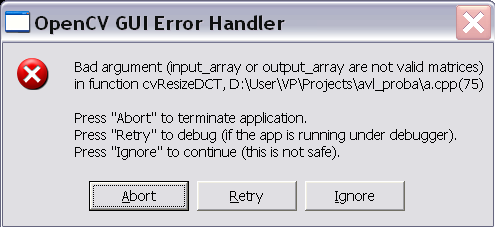
\includegraphics[width=0.5\textwidth]{pics/errmsg.png}

If the error handler is set \texttt{cvStdErrReport}, the above message will be printed to standard error output and program will be terminated or continued, depending on the current error mode.

Error Message printed to Standard Error Output (in \texttt{Leaf} mode)

\begin{verbatim}
OpenCV ERROR: Bad argument (input_array or output_array are not valid matrices)
        in function cvResizeDCT, D:\User\VP\Projects\avl\_proba\a.cpp(75)
Terminating the application...
\end{verbatim}

\subsection{System and Utility Functions}

\cvfunc{Alloc}\label{Alloc}

Allocates memory buffer

\cvexp{
void* cvAlloc( size\_t size );
}{CPP}{PYTHON}

\begin{description}
\cvarg{size}{Buffer size in bytes}
\end{description}

The function \texttt{cvAlloc} allocates \texttt{size} bytes and returns
pointer to the allocated buffer. In case of error the function reports an
error and returns NULL pointer. By default \texttt{cvAlloc} calls
\texttt{icvAlloc} which
itself calls malloc, however it is possible to assign user-defined memory
allocation/deallocation functions using \cross{SetMemoryManager} function.

\cvfunc{Free}\label{Free}

Deallocates memory buffer

\cvexp{

void cvFree( void** ptr );

}{CPP}{PYTHON}

\begin{description}
\cvarg{ptr}{Double pointer to released buffer}
\end{description}

The function \texttt{cvFree} deallocates memory buffer allocated by
\cross{Alloc}. It clears the pointer to buffer upon exit, that is why
the double pointer is used. If \texttt{*buffer} is already NULL, the function
does nothing

\cvfunc{GetTickCount}\label{GetTickCount}

Returns number of ticks

\cvexp{
int64 cvGetTickCount( void );
}{CPP}{PYTHON}

The function \texttt{cvGetTickCount} returns number of ticks starting from some platform-dependent event (number of CPU ticks from the startup, number of milliseconds from 1970th year etc.). The function is useful for accurate measurement of a function/user-code execution time. To convert the number of ticks to time units, use \cross{GetTickFrequency}.

\cvfunc{GetTickFrequency}\label{GetTickFrequency}

Returns number of ticks per microsecond

\cvexp{

double cvGetTickFrequency( void );

}{CPP}{PYTHON}

The function \texttt{cvGetTickFrequency} returns number of ticks per microsecond. Thus, the quotient of \cross{GetTickCount} and \cross{GetTickFrequency} will give a number of microseconds starting from the platform-dependent event.

\cvfunc{RegisterModule}\label{RegisterModule}

Registers another module

\begin{lstlisting}
typedef struct CvPluginFuncInfo
{
    void** func_addr;
    void* default_func_addr;
    const char* func_names;
    int search_modules;
    int loaded_from;
}
CvPluginFuncInfo;

typedef struct CvModuleInfo
{
    struct CvModuleInfo* next;
    const char* name;
    const char* version;
    CvPluginFuncInfo* func_tab;
}
CvModuleInfo;
\end{lstlisting}

\cvexp{
int cvRegisterModule( const CvModuleInfo* module\_info );
}{CPP}{PYTHON}

\begin{description}
\cvarg{module\_info}{Information about the module}
\end{description}

The function \texttt{cvRegisterModule} adds module to the list of
registered modules. After the module is registered, information about
it can be retrieved using \cross{GetModuleInfo} function. Also, the
registered module makes full use of optimized plugins (IPP, MKL, ...),
supported by CXCORE. CXCORE itself, CV (computer vision), CVAUX (auxilary
computer vision) and HIGHGUI (visualization and image/video acquisition) are
examples of modules. Registration is usually done then the shared library
is loaded. See \texttt{cxcore/src/cxswitcher.cpp} and
\texttt{cv/src/cvswitcher.cpp} for details, how registration is done
and look at \texttt{cxcore/src/cxswitcher.cpp}, \texttt{cxcore/src/\_cxipp.h}
on how IPP and MKL are connected to the modules.

\cvfunc{GetModuleInfo}\label{GetModuleInfo}

Retrieves information about the registered module(s) and plugins

\cvexp{
void  cvGetModuleInfo( \par const char* module\_name,\par const char** version,\par const char** loaded\_addon\_plugins );
}{CPP}{PYTHON}

\begin{description}
\cvarg{module\_name}{Name of the module of interest, or NULL, which means all the modules}
\cvarg{version}{The output parameter. Information about the module(s), including version.}
\cvarg{loaded\_addon\_plugins}{The list of names and versions of the optimized plugins that CXCORE was able to find and load}
\end{description}

The function \texttt{cvGetModuleInfo} returns information about one of or
all of the registered modules. The returned information is stored inside
the libraries, so user should not deallocate or modify the returned
text strings.

\cvfunc{UseOptimized}\label{UseOptimized}

Switches between optimized/non-optimized modes

\cvexp{

int cvUseOptimized( int on\_off );

}{CPP}{PYTHON}

\begin{description}
\cvarg{on\_off}{Use optimized ($\ne 0$) or not ($=0$)}
\end{description}

The function \texttt{cvUseOptimized} switches between the mode, where
only pure C implementations from cxcore, OpenCV etc. are used, and
the mode, where IPP and MKL functions are used if available. When
\texttt{cvUseOptimized(0)} is called, all the optimized libraries are
unloaded. The function may be useful for debugging, IPP and MKL upgrade on
the fly, online speed comparisons etc. It returns the number of optimized
functions loaded. Note that by default the optimized plugins are loaded,
so it is not necessary to call \texttt{cvUseOptimized(1)} in the beginning of
the program (actually, it will only increase the startup time)

\cvfunc{SetMemoryManager}\label{SetMemoryManager}

Assings custom/default memory managing functions

\begin{lstlisting}
typedef void* (CV_CDECL *CvAllocFunc)(size_t size, void* userdata);
typedef int (CV_CDECL *CvFreeFunc)(void* pptr, void* userdata);
\end{lstlisting}

\cvexp{
void cvSetMemoryManager( \par CvAllocFunc alloc\_func=NULL,\par CvFreeFunc free\_func=NULL,\par void* userdata=NULL );
}{CPP}{PYTHON}

\begin{description}
\cvarg{alloc\_func}{Allocation function; the interface is similar to \texttt{malloc}, except that \texttt{userdata} may be used to determine the context}
\cvarg{free\_func}{Deallocation function; the interface is similar to \texttt{free}}
\cvarg{userdata}{User data that is transparetly passed to the custom functions}
\end{description}

The function \texttt{cvSetMemoryManager} sets user-defined memory
managment functions (substitutors for malloc and free) that will be called
by cvAlloc, cvFree and higher-level functions (e.g. cvCreateImage). Note,
that the function should be called when there is data allocated using
cvAlloc. Also, to avoid infinite recursive calls, it is not
allowed to call cvAlloc and \cross{Free} from the custom
allocation/deallocation functions.

If \texttt{alloc\_func} and \texttt{free\_func} pointers are
\texttt{NULL}, the default memory managing functions are restored.

\cvfunc{SetIPLAllocators}\label{SetIPLAllocators}

Switches to IPL functions for image allocation/deallocation

\begin{lstlisting}
typedef IplImage* (CV_STDCALL* Cv_iplCreateImageHeader)
                            (int,int,int,char*,char*,int,int,int,int,int,
                            IplROI*,IplImage*,void*,IplTileInfo*);
typedef void (CV_STDCALL* Cv_iplAllocateImageData)(IplImage*,int,int);
typedef void (CV_STDCALL* Cv_iplDeallocate)(IplImage*,int);
typedef IplROI* (CV_STDCALL* Cv_iplCreateROI)(int,int,int,int,int);
typedef IplImage* (CV_STDCALL* Cv_iplCloneImage)(const IplImage*);

#define CV_TURN_ON_IPL_COMPATIBILITY()                                  \
    cvSetIPLAllocators( iplCreateImageHeader, iplAllocateImage,         \
                        iplDeallocate, iplCreateROI, iplCloneImage )
\end{lstlisting}

\cvexp{
void cvSetIPLAllocators( \par
                         Cv\_iplCreateImageHeader create\_header, \par
                         Cv\_iplAllocateImageData allocate\_data, \par
                         Cv\_iplDeallocate deallocate, \par
                         Cv\_iplCreateROI create\_roi, \par
                         Cv\_iplCloneImage clone\_image );
}{CPP}{PYTHON}

\begin{description}
\cvarg{create\_header}{Pointer to iplCreateImageHeader}
\cvarg{allocate\_data}{Pointer to iplAllocateImage}
\cvarg{deallocate}{Pointer to iplDeallocate}
\cvarg{create\_roi}{Pointer to iplCreateROI}
\cvarg{clone\_image}{Pointer to iplCloneImage}
\end{description}


The function \texttt{cvSetIPLAllocators} makes CXCORE to use IPL functions
for image allocation/deallocation operations. For convenience, there
is the wrapping macro \texttt{CV\_TURN\_ON\_IPL\_COMPATIBILITY}. The
function is useful for applications where IPL and CXCORE/OpenCV are used
together and still there are calls to \texttt{iplCreateImageHeader}
etc. The function is not necessary if IPL is called only for data
processing and all the allocation/deallocation is done by CXCORE, or
if all the allocation/deallocation is done by IPL and some of OpenCV
functions are used to process the data.
